%%%%%%%%%%%%%%%%%%%%%%%%%%%%%%%%%%%%%%%%%
% Classicthesis Typographic Thesis
% LaTeX Template
% Version 1.4 (1/1/16)
%
% This template has been downloaded from:
% http://www.LaTeXTemplates.com
%
% Original author:
% André Miede (http://www.miede.de) with commenting modifications by:
% Vel (vel@LaTeXTemplates.com)
%
% License:
% GNU General Public License (v2)
%
% General Tips:
% 1) Make sure to edit the classicthesis-config.file
% 2) New enumeration (A., B., C., etc in small caps): \begin{aenumerate} \end{aenumerate}
% 3) For margin notes: \marginpar or \graffito{}
% 4) Do not use bold fonts in this style, it is designed around them
% 5) Use tables as in the examples
% 6) See classicthesis-preamble.sty for useful commands
%
%%%%%%%%%%%%%%%%%%%%%%%%%%%%%%%%%%%%%%%%%

%----------------------------------------------------------------------------------------
%	PACKAGES AND OTHER DOCUMENT CONFIGURATIONS
%----------------------------------------------------------------------------------------

%twoside,openright,footinclude=true,
\documentclass[
		titlepage,numbers=noenddot,headinclude,%1headlines,
	 	cleardoublepage=empty,
		dottedtoc, % Make page numbers in the table of contents flushed right with dots leading to them
		BCOR=1mm,paper=a4,fontsize=10pt, % Binding correction, paper type and font size
		english, % Languages, change this to your language(s)
		]{scrreprt} 

\setlength{\parindent}{0cm}


%\definecolor{chaptercolor}{green}{0.5}

%\usepackage[Hansen]{fncychap}
            
%%% Change the text block area to add also the margin space
%\setlength{\textwidth}{25pt}
%\areaset[current]{\dimexpr\textwidth+\marginparwidth+\marginparsep}{\textheight}
%\setlength{\marginparwidth}{50pt}
%\setlength{\marginparsep}{0pt}            
             
% Includes the file which contains all the document configurations and packages - make sure to edit this file
%%%%%%%%%%%%%%%%%%%%%%%%%%%%%%%%%%%%%%%%%
% Classicthesis Typographic Thesis
% Configuration File
%
% This file has been downloaded from:
% http://www.LaTeXTemplates.com
%
% Original author:
% André Miede (http://www.miede.de) with extensive commenting changes by:
% Vel (vel@LaTeXTemplates.com)
%
% License:
% GNU General Public License (v2)
%
% Important note:
% The main lines to change in this file are in the DOCUMENT VARIABLES
% section, the rest of the file is for advanced configuration.
%
%%%%%%%%%%%%%%%%%%%%%%%%%%%%%%%%%%%%%%%%%

%----------------------------------------------------------------------------------------
%	CHARACTER ENCODING
%----------------------------------------------------------------------------------------

\PassOptionsToPackage{utf8}{inputenc} % Set the encoding of your files. UTF-8 is the only sensible encoding nowadays. If you can't read äöüßáéçèê∂åëæƒÏ€ then change the encoding setting in your editor, not the line below. If your editor does not support utf8 use another editor!
\usepackage{inputenc}

%----------------------------------------------------------------------------------------
%	DOCUMENT VARIABLES
%	Fill in the lines below to enter your information into the thesis template
%	Each of the commands can be cited anywhere in the thesis
%----------------------------------------------------------------------------------------

% Remove drafting to get rid of the '[ Date - classicthesis version 4.0 ]' text at the bottom of every page
\PassOptionsToPackage{listings,drafting, pdfspacing, subfig,beramono,parts, linedheaders, floatperchapter, eulerchapternumbers}{classicthesis}
%,eulermath
% Available options: drafting parts nochapters linedheaders eulerchapternumbers beramono eulermath pdfspacing minionprospacing tocaligned dottedtoc manychapters listings floatperchapter subfig


\newcommand{\myTitle}{Modeling and simulation of the boiling crisis within PWR at CFD scale\xspace}
\newcommand{\mySubtitle}{Towards Improvements of the Modeling of Wall Boiling for Multiphase CFD Simulations \xspace}
\newcommand{\myDegree}{MsC \xspace}
\newcommand{\myName}{Luc Favre\xspace}
\newcommand{\myProf}{Catherine Colin\xspace}
\newcommand{\myOtherProf}{Stéphane Mimouni\xspace}
\newcommand{\mySupervisor}{Stéphane Pujet\xspace}
\newcommand{\myFaculty}{Toulouse Fluid Mechanics Institute\xspace}
\newcommand{\myCompany}{\'Electricité de France\xspace}
\newcommand{\myDepartment}{Fluid Mechanics, Energy and Environment\xspace}
\newcommand{\myUni}{Institut National Polytechnique de Toulouse\xspace}
\newcommand{\myLocation}{Paris\xspace}
\newcommand{\myTime}{December 2022\xspace}
\newcommand{\myVersion}{version 4.2\xspace}

%----------------------------------------------------------------------------------------
%	USEFUL COMMANDS
%----------------------------------------------------------------------------------------

\newcommand{\ie}{\textit{i.\,e.}\xspace}
\newcommand{\Ie}{\textit{I.\,e.}\xspace}
\newcommand{\eg}{\textit{e.\,g.}\xspace}
\newcommand{\Eg}{\textit{E.\,g.}\xspace} 
\newcommand{\etal}{\textit{et al.}\xspace}

\newcounter{dummy} % Necessary for correct hyperlinks (to index, bib, etc.)
\providecommand{\mLyX}{L\kern-.1667em\lower.25em\hbox{Y}\kern-.125emX\@}
\newlength{\abcd} % for ab..z string length calculation

%----------------------------------------------------------------------------------------
%	PACKAGES
%----------------------------------------------------------------------------------------

\usepackage{lipsum} % Used for inserting dummy 'Lorem ipsum' text into the template

%------------------------------------------------

%\PassOptionsToPackage{ngerman,american}{babel}  % Change this to your language(s)
% Spanish languages need extra options in order to work with this template
%\PassOptionsToPackage{spanish,es-lcroman}{babel}
\usepackage[english]{babel}

%------------------------------------------------			

\usepackage{csquotes}
\PassOptionsToPackage{%
%backend=biber, % Instead of bibtex
backend=bibtex8,bibencoding=ascii,%
language=auto,%
style=numeric-comp,%
url=false,%e
%style=authoryear-comp, % Author 1999, 2010
%bibstyle=authoryear,dashed=false, % dashed: substitute rep. author with ---
sorting=nyt, % name, year, title
maxbibnames=10, % default: 3, et al.
%backref=true,%
natbib=true % natbib compatibility mode (\citep and \citet still work)
}{biblatex}
\usepackage{biblatex}
 
 %------------------------------------------------
%
%\PassOptionsToPackage{fleqn}{amsmath} % Math environments and more by the AMS 
% \usepackage{amsmath}
\usepackage{amsmath}
\usepackage{amssymb}
\usepackage{bm}

\usepackage{gensymb} 




\usepackage{color}
\usepackage{amsmath}
\usepackage{mathtools}
\usepackage{epstopdf}
\usepackage[english]{nomencl}
\usepackage{minitoc}
\usepackage{ifthen}
\usepackage[normalem]{ulem}%\usepackage{ulem}

\usepackage{geometry}
\geometry{
top=20mm,
bottom=20mm,
left=25mm,
right=25mm}
\usepackage{etoolbox}


%%%REMARKS

\usepackage{blindtext}

\usepackage[most]{tcolorbox}

\newtcbtheorem{remark}{\textbf{Remark :} }{
   coltitle=black,
   colback=brown!10,
   colframe=red!70!blue,
   detach title,
   boxrule=0pt,
   leftrule=2pt,
  attach title to upper,
   sharp corners,
   left=1mm,
}{}

\newtcbtheorem{note}{\textbf{Note :} }{
   coltitle=black,
   colback=olive!10!green!10,
   colframe=olive!70!green,
   detach title,
   boxrule=0pt,
   leftrule=2pt,
  attach title to upper,
   sharp corners,
   left=1mm,
}{}
%\newtheorem{remark}{Remark}


%CLICKABLES LINKS
\usepackage[colorlinks]{hyperref}
%\hypersetup{
%	linkcolor=red,
%	citecolor=green,
%	urlcolor=green}



 %------------------------------------------------

\PassOptionsToPackage{T1}{fontenc} % T2A for cyrillics
\usepackage{fontenc}

%------------------------------------------------

\usepackage{textcomp} % Fix warning with missing font shapes

%------------------------------------------------

\usepackage{scrhack} % Fix warnings when using KOMA with listings package  

%------------------------------------------------

\usepackage{xspace} % To get the spacing after macros right

%------------------------------------------------

\usepackage{mparhack} % To get marginpar right

%------------------------------------------------

\usepackage{fixltx2e} % Fixes some LaTeX stuff 

%------------------------------------------------

\PassOptionsToPackage{smaller}{acronym} % Include printonlyused in the first bracket to only show acronyms used in the text
\usepackage{acronym} % Nice macros for handling all acronyms in the thesis

%\renewcommand*{\acsfont}[1]{\textssc{#1}} % For MinionPro
\renewcommand*{\aclabelfont}[1]{\acsfont{#1}}

%------------------------------------------------

\PassOptionsToPackage{pdftex}{graphicx}
\usepackage{graphicx} 
\usepackage{grffile}
\usepackage{xcolor}
%\definecolor{lightred}{red}{0.3}

%------TIKZ PACKAGES
\usepackage{tikz}
\usetikzlibrary{calc}
\usetikzlibrary{math}
\usepackage{pgfplots}
\usetikzlibrary{intersections}


%----------------------------------------------------------------------------------------
%	FLOATS: TABLES, FIGURES AND CAPTIONS SETUP
%----------------------------------------------------------------------------------------

\usepackage{tabularx} % Better tables
\setlength{\extrarowheight}{3pt} % Increase table row height
\newcommand{\tableheadline}[1]{\multicolumn{1}{c}{\spacedlowsmallcaps{#1}}}
\newcommand{\myfloatalign}{\centering} % To be used with each float for alignment
\usepackage{caption}
\captionsetup{font=small}
\usepackage{subfig}  

\usepackage{float}
\usepackage{array}
\usepackage{rotating}
\usepackage{multirow}
\usepackage{multicol}

%----------------------------------------------------------------------------------------
%	CODE LISTINGS SETUP
%----------------------------------------------------------------------------------------

\usepackage{listings} 
%\lstset{emph={trueIndex,root},emphstyle=\color{BlueViolet}}%\underbar} % For special keywords
\lstset{language=[LaTeX]Tex,%C++ % Specify the language(s) for listings here
morekeywords={PassOptionsToPackage,selectlanguage},
keywordstyle=\color{RoyalBlue}, % Add \bfseries for bold
basicstyle=\small\ttfamily, % Makes listings a smaller font size and a different font
%identifierstyle=\color{NavyBlue}, % Color of text inside brackets
commentstyle=\color{Green}\ttfamily, % Color of comments
stringstyle=\rmfamily, % Font type to use for strings
numbers=left, % Change left to none to remove line numbers
numberstyle=\scriptsize, % Font size of the line numbers
stepnumber=5, % Increment of line numbers
numbersep=8pt, % Distance of line numbers from code listing
showstringspaces=false, % Sets whether spaces in strings should appear underlined
breaklines=true, % Force the code to stay in the confines of the listing box
%frameround=ftff, % Uncomment for rounded frame
%frame=single, % Frame border - none/leftline/topline/bottomline/lines/single/shadowbox/L
belowcaptionskip=.75\baselineskip % Space after the "Listing #: Desciption" text and the listing box
}

%----------------------------------------------------------------------------------------
%	HYPERREFERENCES
%----------------------------------------------------------------------------------------

\PassOptionsToPackage{pdftex,hyperfootnotes=false,pdfpagelabels}{hyperref}
\usepackage{hyperref}  % backref linktocpage pagebackref
\pdfcompresslevel=9
\pdfadjustspacing=1

\hypersetup{
% Uncomment the line below to remove all links (to references, figures, tables, etc), useful for b/w printouts
%draft, 
colorlinks=true, linktocpage=true, pdfstartpage=3, pdfstartview=FitV,
% Uncomment the line below if you want to have black links (e.g. for printing black and white)
%colorlinks=false, linktocpage=false, pdfborder={0 0 0}, pdfstartpage=3, pdfstartview=FitV, 
breaklinks=true, pdfpagemode=UseNone, pageanchor=true, pdfpagemode=UseOutlines,%
plainpages=false, bookmarksnumbered, bookmarksopen=true, bookmarksopenlevel=1,%
hypertexnames=true, pdfhighlight=/P,%nesting=true,%frenchlinks,%
urlcolor=webbrown, linkcolor=RoyalBlue, citecolor=webgreen, %pagecolor=RoyalBlue,%
    %urlcolor=Black, linkcolor=Black, citecolor=Black, %pagecolor=Black,%
%------------------------------------------------
% PDF file meta-information
pdftitle={\myTitle},
pdfauthor={\textcopyright\ \myName, \myUni, \myFaculty},
pdfsubject={},
pdfkeywords={},
pdfcreator={pdfLaTeX},
pdfproducer={LaTeX with hyperref and classicthesis}
%------------------------------------------------
}

%----------------------------------------------------------------------------------------
%	AUTOREFERENCES SETUP
%	Redefines how references in text are prefaced for different 
%	languages (e.g. "Section 1.2" or "section 1.2")
%----------------------------------------------------------------------------------------

\makeatletter
%\@ifpackageloaded{babel}
%{
%\addto\extrasamerican{
%\renewcommand*{\figureautorefname}{Figure}
%\renewcommand*{\tableautorefname}{Table}
%\renewcommand*{\partautorefname}{Part}
%\renewcommand*{\chapterautorefname}{Chapter}
%\renewcommand*{\sectionautorefname}{Section}
%\renewcommand*{\subsectionautorefname}{Section}
%\renewcommand*{\subsubsectionautorefname}{Section}
%}
%\addto\extrasngerman{
%\renewcommand*{\paragraphautorefname}{Absatz}
%\renewcommand*{\subparagraphautorefname}{Unterabsatz}
%\renewcommand*{\footnoteautorefname}{Fu\"snote}
%\renewcommand*{\FancyVerbLineautorefname}{Zeile}
%\renewcommand*{\theoremautorefname}{Theorem}
%\renewcommand*{\appendixautorefname}{Anhang}
%\renewcommand*{\equationautorefname}{Gleichung}
%\renewcommand*{\itemautorefname}{Punkt}
%}
%\providecommand{\subfigureautorefname}{\figureautorefname} % Fix to getting autorefs for subfigures right
%}{\relax}
\makeatother

%----------------------------------------------------------------------------------------

\usepackage{classicthesis} 

%----------------------------------------------------------------------------------------
%	CHANGING TEXT AREA 
%----------------------------------------------------------------------------------------

%\linespread{1.05} % a bit more for Palatino
%\areaset[current]{312pt}{761pt} % 686 (factor 2.2) + 33 head + 42 head \the\footskip
%\setlength{\marginparwidth}{7em}%
%\setlength{\marginparsep}{2em}%

%----------------------------------------------------------------------------------------
%	USING DIFFERENT FONTS
%----------------------------------------------------------------------------------------

%\usepackage[oldstylenums]{kpfonts} % oldstyle notextcomp
%\usepackage[osf]{libertine}
%\usepackage[light,condensed,math]{iwona}
%\renewcommand{\sfdefault}{iwona}
\usepackage{lmodern} % <-- no osf support :-(
%\usepackage{cfr-lm} % 
%\usepackage[urw-garamond]{mathdesign} <-- no osf support :-(
%\usepackage[default,osfigures]{opensans} % scale=0.95 
%\usepackage[sfdefault]{FiraSans}

\addbibresource{Bibliography.bib} % The file housing your bibliography
%\addbibresource[label=ownpubs]{Self_Publications.bib} % Uncomment for optional self-publications

%\hyphenation{Put special hyphenation here}

\begin{document}

\frenchspacing % Reduces space after periods to make text more compact

\raggedbottom % Makes all pages the height of the text on that page

%\selectlanguage{american} % Select your default language - e.g. american or ngerman

%\renewcommand*{\bibname}{new name} % Uncomment to change the name of the bibliography
%\setbibpreamble{} % Uncomment to include a preamble to the bibliography - some text before the reference list starts

\pagenumbering{roman} % Roman page numbering prior to the start of the thesis content (i, ii, iii, etc)

\pagestyle{plain} % Suppress headers for the pre-content pages


\newcommand{\HRule}{\rule{\linewidth}{0.5mm}}
\newcommand{\npar}{\vspace{\baselineskip}}


%Derivatives
\newcommand{\dtime}[1]{\frac{\partial{#1}}{\partial t}}
\newcommand{\dpartial}[2]{\frac{\partial #1}{\partial #2}}
\newcommand{\derive}[2]{\frac{\mathrm{d}#1}{\mathrm{d}#2}}


%%Tensor Calculation
%\newcommand{\vect}[1]{\overline{\boldsymbol{#1}}}
\newcommand{\vect}[1]{\overline{#1}}

\newcommand{\tens}[1]{\overline{\overline{#1}}}
%\newcommand{\tens}[1]{\overline{\overline{\boldsymbol{#1}}}}

\newcommand{\divg}[1]{\vect{\nabla} \cdot \left({#1}\right)}
%\newcommand{\divg}[1]{\nabla\cdot\left(#1\right)}
\newcommand{\vecdivg}[1]{{\tens{\nabla }\cdot \left({#1}\right)}}

%\newcommand{\grad}[1]{\overline{\boldsymbol{\nabla}}#1}
\newcommand{\grad}[1]{\overline{\nabla}\left({#1}\right)}
\newcommand{\vecgrad}[1]{\overline{\overline{\nabla}}\left({#1}\right)}

%\newcommand{\gradtens}[1]{\overline{\overline{\boldsymbol{\nabla}}}#1}
\newcommand{\gradtens}[1]{\overline{\overline{{\nabla}}}#1}


%\newcommand{\lapla}[1]{\overline{\boldsymbol{\Delta}}#1}
\newcommand{\lapla}[1]{\overline{{\Delta}}#1}

\newcommand{\inv}[1]{\frac{1}{#1}}

\newcommand{\rot}[1]{\overline{\nabla}\wedge{#1}}




%\newcommand{\debm}{\mathrm{kg}.\mathrm{m}^{-2}.\mathrm{s}^{-1}}
\newcommand{\debm}{\text{kg/m$^{2}$/s}}


\newcommand{\parth}[1]{\left( #1 \right)}
\newcommand{\crocht}[1]{\left[ #1 \right]}
\newcommand{\bars}[1]{\left| #1 \right|}
\newcommand{\up}[1]{$^\mathrm{#1}$}
\newcommand{\norm}[1]{\left|\left|{#1}\right|\right|}

\renewcommand{\max}[1]{\mathrm{max}\parth{#1}}
\renewcommand{\min}[1]{\mathrm{min}\parth{#1}}


%%Non-dimensional numbers
\newcommand{\Ja}{\mathrm{Ja}}
\renewcommand{\Re}{\mathrm{Re}}
\renewcommand{\Pr}{\mathrm{Pr}}
\newcommand{\Nu}{\mathrm{Nu}}
\newcommand{\Fr}{\mathrm{Fr}}
\newcommand{\Eo}{\mathrm{Eo}}
\newcommand{\St}{\mathrm{St}}
\newcommand{\We}{\mathrm{We}}
\newcommand{\Pe}{\mathrm{Pe}}
\newcommand{\Ca}{\mathrm{Ca}}
\newcommand{\Sr}{\mathrm{Sr}}
\newcommand{\Bo}{\mathrm{Bo}}


%Trigonometry
\newcommand{\dalpha}{\mathrm{d}\alpha}
\newcommand{\dtheta}{\mathrm{d}\theta}

\newcommand{\trb}{\mathrm{tr}\parth{\beta}}

\renewcommand{\cos}[1]{\mathrm{cos}\parth{#1}}
\renewcommand{\sin}[1]{\mathrm{sin}\parth{#1}}
\newcommand{\cossq}[1]{\mathrm{cos}^{2}\parth{#1}}
\newcommand{\sinsq}[1]{\mathrm{sin}^{2}\parth{#1}}
\renewcommand{\ln}[1]{\mathrm{ln}\parth{#1}}
\renewcommand{\exp}[1]{\mathrm{exp}\parth{#1}}
\renewcommand{\tanh}[1]{\mathrm{tanh}\parth{#1}}

%Color maths
\newcommand{\redmath}[1]{\begingroup\color{red}#1\endgroup}
\newcommand{\orangemath}[1]{\begingroup\color{orange!80!black}#1\endgroup}
\newcommand{\yellowmath}[1]{\begingroup\color{yellow}#1\endgroup}
\newcommand{\bluemath}[1]{\begingroup\color{blue}#1\endgroup}
\newcommand{\greenmath}[1]{\begingroup\color{olive!70!black}#1\endgroup}


%\newcommand{\etal}{\textit{et al.}}
%\newcommand{\ie}{\textit{i.e.}}
%\newcommand{\eg}{\textit{e.g.}}



%----------------------------------------------------------------------------------------
%	PRE-CONTENT THESIS PAGES
%----------------------------------------------------------------------------------------

% Title Page

\begin{titlepage}


\includepdf{cover_megep.pdf}

%\begin{addmargin}[-1cm]{-3cm}
\begin{center}
\large

\hfill
\vfill

{
\color{Maroon}\spacedallcaps{\myTitle} \\ %\bigskip % Thesis title
}

\spacedlowsmallcaps{\myName} % Your name

\vfill

%
\includegraphics[width=6cm]{gfx/TFZsuperellipse_bw} \\ \medskip % Picture

\mySubtitle \\ \medskip % Thesis subtitle
%\myDegree \\
%\myDepartment \\
%\myFaculty \\
%\myUni \\ \bigskip

\myLocation , \myTime % Time and version

\vfill

\end{center}
%\end{addmargin}

\end{titlepage} % Main title page

% Back of the title page

\thispagestyle{empty}

\hfill

\vfill

\noindent\myName: \textit{\myTitle,} \mySubtitle, \myTime

% You may wish to do something with the back of the title page, such as including your supervisors, location or time frame of the work. Below is an example of doing so although you may want to tweak it to your liking.

%\bigskip

%\noindent\spacedlowsmallcaps{Supervisors}: \\
%\myProf \\
%\myOtherProf \\ 
%\mySupervisor

%\medskip \\

%\noindent\spacedlowsmallcaps{Location}: \\
%\myLocation

%\medskip \\

%\noindent\spacedlowsmallcaps{Time Frame}: \\
%\myTime
 % Back of the title page

\cleardoublepage% Dedication

\thispagestyle{empty}
\refstepcounter{dummy}

\pdfbookmark[1]{Dedication}{Dedication} % Bookmark name visible in a PDF viewer

\vspace*{3cm}

\begin{center}
test
%"If the facts don't fit the theory, change the facts." \\ \medskip
%--- Unkown wise man   
\end{center} % Dedication page

%\cleardoublepage% Publications - a page listing research articles written using content in the thesis

\pdfbookmark[1]{To the reader}{To the reader} % Bookmark name visible in a PDF viewer

\chapter*{To the reader} % Publications page text


Dear reader,

\npar

This small section aims to detail and acknowledge some of the tools I used during my PhD to produce this work :

\begin{itemize}

\setlength{\itemsep}{10pt}

\item This thesis has been written using \LaTeX with TeXmaker (\url{https://www.xm1math.net/texmaker/}) along with the MikTeX distribution (\url{https://miktex.org/}), based on the \texttt{classicthesis} package (\url{https://ctan.org/pkg/classicthesis}).

\item The bibliography has been handled using Zotero (\url{https://www.zotero.org/}).

\item All the models used outside of CFD computations have been developed using Python 3 (\url{https://www.python.org/}).

\item Most of the figures in this manuscript have been drawn using the Python 3 package \texttt{matplotlib} (\url{https://matplotlib.org/}) or the \LaTeX package TikZ (\url{https://tikz.net/}).

\item Fluid properties in Python 3 models have been computed using the \texttt{CoolProp} package (\url{http://www.coolprop.org/}):

\small{
Bell Ian H., Wronski Jorrit, Quoilin Sylvain and Lemort Vincent, Pure and Pseudo-pure Fluid Thermophysical Property Evaluation and the Open-Source Thermophysical Property Library CoolProp, Industrial \& Engineering Chemistry Research, 53-6 (pp. 2498--2508), 2014, doi:\url{10.1021/ie4033999}, \url{http://pubs.acs.org/doi/abs/10.1021/ie4033999}
}


\end{itemize}


\npar

\npar

You will find some extra documentation as well as some appendices to this work on my personal website \url{https://www.lfavre.org/} (still to be updated, it should be ready in a couple of months).

\npar

\npar

If you notice any mistake in the core of the document, if you have any question regarding this work, or if you would like to obtain data, Python programs or results, \textbf{feel absolutely free to contact me at my permanent mail address}:

\begin{center}
\large
\href{mailto:favre.luc05@gmail.com}{favre.luc05@gmail.com}
\end{center}


\npar

\npar

I hope you will enjoy reading this thesis ! {\Large{ \smiley{} }}

 % Uncomment and create a Foreword.tex to include a foreword

\cleardoublepage% Abstract

%\renewcommand{\abstractname}{Abstract} % Uncomment to change the name of the abstract

\pdfbookmark[1]{Abstract}{Abstract} % Bookmark name visible in a PDF viewer

\begingroup
\let\clearpage\relax
\let\cleardoublepage\relax
\let\cleardoublepage\relax

\chapter*{Abstract}

In Pressurized Water Reactors (PWR), the heat released by the nuclear fuel is transferred to the water flowing in the primary circuit, which is pressurized at 150 bar to avoid boiling. However, water can sometimes reach the Onset of Nucleate Boiling (ONB) under accident conditions that can further lead to the Boiling Crisis. At this point, an instantaneous transition between nucleate and film boiling occurs, inducing the formation of a vapor blanket around the fuel rods which acts as a thermal insulation and  causes a rapid rise of their temperature, posing a risk of fuel cladding damage. Prediction of the Critical Heat Flux (corresponding to Boiling Crisis occurrence) is thus a primal safety stake, currently achieved using dedicated experimental correlations that do not include detailed description of the boiling physics.

\npar

This thesis aims to study the modeling of the boiling physics at a local scale, so-called  “CFD” (Computational Fluid Dynamics), which allows simulating boiling flows using a millimeter spatial discretization. The in-house code NEPTUNE\_CFD is the reference tool used by EDF R\&D to investigate the local-scale multiphase physics.

\npar

First, simulations of boiling flows in a vertical tube are achieved using NEPTUNE\_CFD. Results are compared to the DEBORA experiment (flow boiling of refrigerant R12 that mimics PWR dimensionless numbers) in conditions representative of the industrial situation. The results show a global agreement with the measurements, but display significant discrepancies regarding bubble diameter and wall temperature. The latter is computed through the wall boiling model of NEPTUNE\_CFD called “Heat Flux Partitioning”, which splits the wall heat flux between different heat transfer mechanisms (convection, phase change, transient conduction, etc.).

\npar

The main objective of the thesis then consisted in the development of a new Heat Flux Partitioning model in order to account for a more extensive descriptions of the boiling phenomena, including notably the effect of bubble sliding. A fine modeling of bubble dynamics at the wall has been proposed thorough a mechanistic approach based on a force balance over the bubble. Forces at stake have been reassessed (drag, added mass, etc.) and allowed satisfactory prediction of bubble detachment diameter as well as sliding velocity at low and high pressure. The Heat Flux Partitioning model has been completed by conducting a precise evaluation of the numerous required closure laws (waiting time, nucleation site density, etc.) through comparisons with experimental measurements from the literature. The newly assembled model has finally been validated against wall temperature measurements and implemented in NEPTUNE\_CFD.

\npar

The Critical Heat Flux prediction in anchored as a perspective of this framework. Recent experiments showed that the Boiling Crisis can be described using physical parameters involved in the Heat Flux Partitioning formulation. A criterion based on the proportion of wall area covered by bubbles has further been tested using the old NEPTUNE\_CFD formulation and showed a coherent qualitative behavior.

\npar

Finally, the focus was put on a configuration consisting of a tube with mixing vanes similar to those present in PWR cores. Results of NEPTUNE\_CFD simulations showed significant discrepancy regarding core void fraction prediction. Single-phase flow simulations of the same case displayed an overestimation of the liquid’s rotation, which could explain the too large vapor gathering at the center for the boiling cases. 

\endgroup		

\npar

\npar

\textbf{\underline{keywords :}} phase change, heat transfer, fluid mechanics, multiphase flows, numerical simulations

\vfill % Abstract page

\cleardoublepage% Publications - a page listing research articles written using content in the thesis

\pdfbookmark[1]{Publications}{Publications} % Bookmark name visible in a PDF viewer

\chapter*{Publications} % Publications page text

\npar
\npar


\textsc{Conference Proceedings}
\npar

\hrule

\npar
\npar

Luc \textsc{Favre}, Stéphane \textsc{Pujet}, Stéphane \textsc{Mimouni} and Catherine \textsc{Colin}, \textit{NEPTUNE\_CFD Simulations of DEBORA-Promoteur experiments : Boiling Freon in a Vertical Pipe with Mixing Vanes}, \ul{Proceedings of the 19\textsuperscript{th} International Topical Meeting on Nuclear Reactor Thermal Hydraulics} (NURETH 19), Brussels, Belgium, 2022

\npar
\npar

Luc \textsc{Favre}, Catherine \textsc{Colin}, Stéphane \textsc{Pujet} and Stéphane \textsc{Mimouni} , \textit{An Analytical Approach of Bubble Departure by Sliding in Vertical Flow Boiling}, \ul{Advances in Thermal Hydraulics 2022} (ATH 2022), Anaheim, CA, USA, 2022


\npar
\npar
\npar
\npar
\npar

\textsc{Journal Papers}
\npar

\hrule

\npar
\npar

Luc \textsc{Favre}, Catherine \textsc{Colin}, Stéphane \textsc{Pujet} and Stéphane \textsc{Mimouni}, \textit{An updated force balance approach to investigate bubble sliding in vertical flow boiling at low and high pressures}, \ul{International Journal of Heat and Mass Transfer}, 211, 124227, 2023, \url{10.1016/j.ijheatmasstransfer.2023.124227}

\npar
\npar

And probably an other paper on Heat Flux Partitioning currently in preparation... {\Large{ \smiley{} }} % Publications from the thesis page

\cleardoublepage% Acknowledgements

\pdfbookmark[1]{Acknowledgements / Remerciements}{Acknowledgements / Remerciements} % Bookmark name visible in a PDF viewer

\begin{flushleft}{\slshape    
Great success !} \\ \medskip
--- \textbf{Borat Sagdiyev}
\end{flushleft}
\begin{flushright}{\slshape    
Science sans conscience n'est que ruine de l'âme.} \\ \medskip
--- \textbf{Fran\c{c}ois Rabelais}
\end{flushright}

\npar




\bigskip

%----------------------------------------------------------------------------------------

\begingroup

\let\clearpage\relax
\let\cleardoublepage\relax
\let\cleardoublepage\relax

\chapter*{Acknowledgements / Remerciements}

Après trois années de doctorat, je me demande si la section des remerciements n'est pas parmi celles auxquelles j'ai le plus réfléchi. Chaque moment passé avec des proches ou petite pensée nostalgique n'incite qu'à ajouter une ligne pour quelqu'un. Cette thèse ne fera donc pas exception : préparez-vous pour des remerciements à rallonge ! 

\npar

Mes premières penseés vont évidemment à mes trois encadrants avec qui j'ai eu la chance de travailler pendant ces trois années : Catherine, Stéphane P. et Stéphane M. Leurs qualités tant scientifiques qu'humaines ont clairement été les piliers de ces travaux de doctorat.

\npar
Catherine, il va sans dire que cette thèse n'aurait pas connu cet aboutissement sans ton expérience et ton regard affuté sur la physique des écoulements multiphasiques et des changements de phase. En plus d'être la "spécialiste de bulles" (comme j'aimais le dire à mes proches), ta gentillesse, ton humanité et ta présence ont été d'une aide inestimable et je t'en suis profondément reconnaissant. T'avoir comme directrice de thèse fut une réelle chance et est sans aucun doune une des principales raisons m'ayant donné l'envie de m'essayer à une carrière académique ! J'espère sincèrement pouvoir à nouveau échanger et travailler avec toi à l'avenir.

\npar

Stéphane P., avec qui je ne compte plus les discussions captivantes tant autour du nucléaire que de la science en général ou encore de politique depuis que je suis arrivé en stage dans le groupe I8C.  Ton soutien permanent durant ces trois années, la liberté d'action que tu m'as laissée ainsi que tes remarques et ton expertise d'une pertinence rare ont su me laisser appréhender le travail de recherche dans les meilleures conditions possibles. En ajoutant à cela tous les très bon moments passés ensemble que ça soit de la salle café jusque dans les rues de Los Angeles, tu es à la fois un collègue, un tuteur et un ami aux multiples qualités. Merci infiniment pour tout.

Stéphane M., 



\noindent Put your acknowledgements here.\\

\noindent Many thanks to everybody who already sent me a postcard!\\

\noindent Regarding the typography and other help, many thanks go to Marco Kuhlmann, Philipp Lehman, Lothar Schlesier, Jim Young, Lorenzo Pantieri and Enrico Gregorio\footnote{Members of GuIT (Gruppo Italiano Utilizzatori di \TeX\ e \LaTeX )}, J\"org Sommer, Joachim K\"ostler, Daniel Gottschlag, Denis Aydin, Paride Legovini, Steffen Prochnow, Nicolas Repp, Hinrich Harms, Roland Winkler, and the whole \LaTeX-community for support, ideas and some great software.

\bigskip

\noindent\emph{Regarding \mLyX}: The \mLyX\ port was initially done by
\emph{Nicholas Mariette} in March 2009 and continued by
\emph{Ivo Pletikosi\'c} in 2011. Thank you very much for your work and the contributions to the original style.

\endgroup % Acknowledgements page

\pagestyle{scrheadings} % Show chapter titles as headings

\cleardoublepage% Table of Contents - List of Tables/Figures/Listings and Acronyms

\refstepcounter{dummy}

\pdfbookmark[1]{\contentsname}{tableofcontents} % Bookmark name visible in a PDF viewer

\setcounter{tocdepth}{2} % Depth of sections to include in the table of contents - currently up to subsections

\setcounter{secnumdepth}{3} % Depth of sections to number in the text itself - currently up to subsubsections

\manualmark
\markboth{\spacedlowsmallcaps{\contentsname}}{\spacedlowsmallcaps{\contentsname}}
\tableofcontents 
\automark[section]{chapter}
\renewcommand{\chaptermark}[1]{\markboth{\spacedlowsmallcaps{#1}}{\spacedlowsmallcaps{#1}}}
\renewcommand{\sectionmark}[1]{\markright{\thesection\enspace\spacedlowsmallcaps{#1}}}

\clearpage

\begingroup 
\let\clearpage\relax
\let\cleardoublepage\relax
\let\cleardoublepage\relax

%----------------------------------------------------------------------------------------
%	List of Figures
%----------------------------------------------------------------------------------------

\refstepcounter{dummy}
%\addcontentsline{toc}{chapter}{\listfigurename} % Uncomment if you would like the list of figures to appear in the table of contents
\pdfbookmark[1]{\listfigurename}{lof} % Bookmark name visible in a PDF viewer

\listoffigures

\vspace{8ex}
\newpage

%----------------------------------------------------------------------------------------
%	List of Tables
%----------------------------------------------------------------------------------------

\refstepcounter{dummy}
%\addcontentsline{toc}{chapter}{\listtablename} % Uncomment if you would like the list of tables to appear in the table of contents
\pdfbookmark[1]{\listtablename}{lot} % Bookmark name visible in a PDF viewer

\listoftables
        
\vspace{8ex}
\newpage
    
%----------------------------------------------------------------------------------------
%	List of Listings
%---------------------------------------------------------------------------------------- 

\refstepcounter{dummy}
%\addcontentsline{toc}{chapter}{\lstlistlistingname} % Uncomment if you would like the list of listings to appear in the table of contents
\pdfbookmark[1]{\lstlistlistingname}{lol} % Bookmark name visible in a PDF viewer

\lstlistoflistings 

\vspace{8ex}
\newpage
       
%----------------------------------------------------------------------------------------
%	Acronyms & Nomenclaure
%----------------------------------------------------------------------------------------
    

%Latin symbols
\nomenclature[latin]{$G$}{Mass flux [$\debm$]}
\nomenclature[latin]{$R$}{Bubble radius [m]}
\nomenclature[latin]{$R_{c}$}{Bubble curvature radius [m]}
\nomenclature[latin]{$r_{w}$}{Bubble foot radius [m]}
\nomenclature[latin]{$D$}{Bubble diameter [m]}
\nomenclature[latin]{$D_{h}$}{Hydraulic diameter [m]}
\nomenclature[latin]{$l_{sl}$}{Bubble sliding length [m]}
\nomenclature[latin]{$F$}{Force [N]}
\nomenclature[latin]{$g$}{Gravity acceleration [m\up{2}/s]}
\nomenclature[latin]{$V$}{Volume [m\up{3}]}
\nomenclature[latin]{$T$}{Temperature [K]}
\nomenclature[latin]{$C$}{Force coefficient [-]}
\nomenclature[latin]{$U$}{Velocity [m/s]}
\nomenclature[latin]{$U_{\tau}$}{Wall friction velocity [m/s]}
\nomenclature[latin]{$U_{rel}=U_{L}-U_{b}$}{Relative velocity [m/s]}
\nomenclature[latin]{$E$}{Kinetic energy [J]}
\nomenclature[latin]{$K$}{Bubble growth constant [-]}
\nomenclature[latin]{$h_{LV}$}{Latent heat of vaporization [J/kg]}
\nomenclature[latin]{$L_{c}=\sqrt{\frac{\sigma}{\parth{\rho_{L}-\rho_{V}}g}}$}{Capillary length [m]}

%Non-Dimensional numbers
\nomenclature[ND]{$\Re_{b}=\frac{U_{rel}D_{b}}{\nu_{L}}$}{Bubble Reynolds number [-]}
\nomenclature[ND]{$\Re_{D_{h}}=\frac{G_{L}D_{h}}{\mu_{L}}$}{Liquid bulk Reynolds number [-]}
\nomenclature[ND]{$\Sr =\frac{2 \gamma R}{\bars{U_{rel}}}$}{Non-dimensional shear rate [-]}
\nomenclature[ND]{$\Ja =\frac{\rho_{L}c_{P,L}\bars{T-T_{sat}}}{\rho_{V}h_{LV}}$}{Jakob number [-]}
\nomenclature[ND]{$\Pr =\frac{\nu}{\eta}$}{Prandtl number [-]}
\nomenclature[ND]{$\Fr =\frac{\rho_{L}U_{L}^{2}}{\parth{\rho_{L}-\rho_{V}}gR}$}{Froude number [-]}
\nomenclature[ND]{$\Eo =\frac{\parth{\rho_{L}-\rho_{V}}gR^{2}}{\sigma}$}{Eotvos number [-]}
\nomenclature[ND]{$\Ca =\frac{\mu_{L}U_{L}}{\sigma}$}{Capillary number [-]}
\nomenclature[ND]{$y^{+} =\frac{yU_{\tau}}{\nu_{L}}$}{Non-dimensional wall distance [-]}

%Greek symbols
\nomenclature[grec]{$\phi$}{Heat flux [J/m\up{2}/s]}
\nomenclature[grec]{$\eta$}{Thermal diffusivity[m\up{2}/s]}
\nomenclature[grec]{$\mu$}{Dynamic viscosity [J.s/m\up{-3}]}
\nomenclature[grec]{$\nu$}{Kinematic viscosity [m\up{2}/s]}
\nomenclature[grec]{$\gamma$}{Shear rate [s\up{-1}]}
\nomenclature[grec]{$\lambda$}{Thermal conductivity [W/m/K]}
\nomenclature[grec]{$\sigma$}{Surface tension [J/m\up{2}]}
\nomenclature[grec]{$\rho$}{Density [kg/m\up{3}]}
\nomenclature[grec]{$\theta$, $\dtheta$}{Contact angle and half-hysteresis [$\degree$ or rad]}
\nomenclature[grec]{$\theta_{i}$}{Bubble inclination angle [$\degree$ or rad]}

%Subscripts
\nomenclature[subscript]{$L$}{Liquid or Lift}
\nomenclature[subscript]{$V$}{Vapor}
\nomenclature[subscript]{$D$}{Drag}
\nomenclature[subscript]{$AM$}{Added-Mass}

\nomenclature[subscript]{$d$}{Departure or Downstream}
\nomenclature[subscript]{$lo$}{Lift-off}
\nomenclature[subscript]{$u$}{upstream}
\nomenclature[subscript]{$b$}{Bubble}
\nomenclature[subscript]{$w$}{Wall}
\nomenclature[subscript]{$sat$}{Saturation}


%Acronyms
\nomenclature[acronym]{PWR}{Pressurized Water Reactor}
\nomenclature[acronym]{SMR}{Small Modular Reactor}
\nomenclature[acronym]{CHF}{Critical Heat Flux}
\nomenclature[acronym]{BC}{Boiling Crisis}
\nomenclature[acronym]{HFP}{Heat Flux Partitioning}
\nomenclature[acronym]{DNS}{Direct Numerical Simulations}
\nomenclature[acronym]{RPE}{Rayleigh-Plesset Equation}


\printnomenclature[1in]
       
       
%----------------------------------------------------------------------------------------
%	Acronyms
%----------------------------------------------------------------------------------------

\refstepcounter{dummy}
%\addcontentsline{toc}{chapter}{Acronyms} % Uncomment if you would like the acronyms to appear in the table of contents
\pdfbookmark[1]{Acronyms}{acronyms} % Bookmark name visible in a PDF viewer

\markboth{\spacedlowsmallcaps{Acronyms}}{\spacedlowsmallcaps{Acronyms}}


\chapter*{Acronyms}

\begin{acronym}[UML]
\acro{CFD}{Computational Fluid Dynamics}
\acro{CMFD}{Computational Multi-Fluid Dynamics}
\acro{NCFD}{NEPTUNE\_CFD}
\acro{DNS}{Direct Numerical Simulation}
\acro{NSD}{Nucleation Site Density}
\end{acronym}  

\chapter*{Nomenclature}


\begin{tabular}{l c r}

$N_{sit,0}$ & Nucleation Site Density computed by correlation & [$\mathrm{m}^{-2}$]

\end{tabular}


\endgroup % Contents, list of figures/tables/listings and acronyms

\cleardoublepage

\pagenumbering{arabic} % Arabic page numbering for thesis content (1, 2, 3, etc)
%\setcounter{page}{90} % Uncomment to manually start the page counter at an arbitrary value (for example if you wish to count the pre-content pages in the page count)

\cleardoublepage % Avoids problems with pdfbookmark

%----------------------------------------------------------------------------------------
%	THESIS CONTENT - CHAPTERS
%----------------------------------------------------------------------------------------

%\ctparttext{You can put some informational part preamble text here. Illo principalmente su nos. Non message \emph{occidental} angloromanic da. Debitas effortio simplificate sia se, auxiliar summarios da que, se avantiate publicationes via. Pan in terra summarios, capital interlingua se que. Al via multo esser specimen, campo responder que da. Le usate medical addresses pro, europa origine sanctificate nos se.} % Text on the Part 1 page describing  the content in Part 1

\part{Introduction} % First part of the thesis

%% Chapter 1

\chapter{Introduction} % Chapter title

\label{ch:introduction} % For referencing the chapter elsewhere, use \autoref{ch:introduction} 

%----------------------------------------------------------------------------------------

This template for \LaTeX\ has two goals:
\begin{enumerate}
\item Provide students with an easy-to-use template for their Master's or PhD thesis (though it might also be used by other types of authors for reports, books, etc.).
\item Provide a classic, high-quality typographic style that is inspired by \citeauthor{bringhurst:2002}'s ``\emph{The Elements of Typographic Style}'' \citep{bringhurst:2002}.
\marginpar{\myTitle \myVersion}
\end{enumerate}

The bundle is configured to run with a \emph{full} MiK\TeX\ or \TeX Live installation right away and, therefore, it uses only freely available fonts.

People interested only in the nice style and not the whole bundle can now use the style stand-alone via the file \texttt{classicthesis.sty}. This works now also with ``plain'' \LaTeX.

As of version 3.0, \texttt{classicthesis} can also be easily used with \mLyX\footnote{\url{http://www.lyx.org}} thanks to Nicholas Mariette and Ivo Pletikosi\'c. The \mLyX\ version of this manual will contain more information on the details.

This should enable anyone with a basic knowledge of \LaTeXe\ or \mLyX\ to produce beautiful documents without too much effort. In the end, this is my overall goal: more beautiful documents, especially theses, as I am tired of seeing so many ugly ones.

The whole template and the used style is released under the \textsmaller{GNU} General Public License. 

If you like the style then I would appreciate a postcard:
\begin{center}
André Miede \\
Detmolder Straße 32 \\
31737 Rinteln \\
Germany
\end{center}

\noindent The postcards I received so far are available at:
\begin{center}
 \url{http://postcards.miede.de}
\end{center}
\marginpar{A well-balanced line width improves the legibility of the text. That's what typography is all about, right?} So far, many theses, some books, and several other publications have been typeset successfully with it. If you are interested in some typographic details behind it, enjoy Robert Bringhurst's wonderful book. % \citep{bringhurst:2002}.

\paragraph{Important Note:} Some things of this style might look unusual at first glance, many people feel so in the beginning. However, all things are intentionally designed to be as they are, especially these:
\begin{itemize}
\item No bold fonts are used. Italics or spaced small caps do the job quite well.
\item The size of the text body is intentionally shaped like it is. It supports both legibility and allows a reasonable amount of information to be on a page. And, no: the lines are not too short.
\item The tables intentionally do not use vertical or double rules. See the documentation for the \texttt{booktabs} package for a nice discussion of this topic.\footnote{To be found online at \\ \url{http://www.ctan.org/tex-archive/macros/latex/contrib/booktabs/}.}
\item And last but not least, to provide the reader with a way easier access to page numbers in the table of contents, the page numbers are right behind the titles. Yes, they are \emph{not} neatly aligned at the right side and they are \emph{not} connected with dots that help the eye to bridge a distance that is not necessary. If you are still not convinced: is your reader interested in the page number or does she want to sum the numbers up?
\end{itemize}

\noindent Therefore, please do not break the beauty of the style by changing these things unless you really know what you are doing! Please.

\paragraph{Yet Another Important Note:} Since \texttt{classicthesis}' first release in 2006, many things have changed in the \LaTeX\ world.  Trying to keep up-to-date, \texttt{classicthesis} grew and evolved into many directions, trying to stay (some kind of) stable and be compatible with its port to \mLyX. However, there are still many remains from older times in the code, many dirty workarounds here and there, and several other things I am absolutely not proud of (for example my unwise combination of \acsfont{KOMA} and \texttt{titlesec} etc.). \graffito{An outlook into the future of \texttt{classicthesis}.}

Currently, I am looking into how to completely re-design and re-implement \texttt{classicthesis} making it easier to maintain and to use. As a general idea, \texttt{classicthesis.sty} should be developed and distributed separately from the template bundle itself. Excellent spin-offs such as \texttt{arsclassica} could also be integrated (with permission by their authors) as format configurations. Also, current trends of \texttt{microtype}, \texttt{fontspec}, etc. should be included as well. As I am not really into deep \LaTeX\ programming, I will reach out to the \LaTeX\ community for their expertise and help.

%----------------------------------------------------------------------------------------

\section{Organization}
A very important factor for successful thesis writing is the organization of the material. This template suggests a structure as the following:
\begin{itemize}
\marginpar{You can use these margins for summaries of the text body\dots}
\item\texttt{Chapters/} is where all the ``real'' content goes in separate files such as \texttt{Chapter01.tex} etc.
\item\texttt{FrontBackMatter/} is where all the stuff goes that surrounds the ``real'' content, such as the acknowledgments, dedication, etc.
\item\texttt{gfx/} is where you put all the graphics you use in the thesis. Maybe they should be organized into subfolders depending on the chapter they are used in, if you have a lot of graphics.
\item\texttt{Bibliography.bib}: the Bib\TeX\ database to organize all the references you might want to cite.
\item\texttt{classicthesis.sty}: the style definition to get this awesome look and feel. Bonus: works with both \LaTeX\ and \textsc{pdf}\LaTeX\dots and \mLyX.
\item\texttt{ClassicThesis.tcp} a \TeX nicCenter project file. Great tool and it's free!
\item\texttt{ClassicThesis.tex}: the main file of your thesis where all the content gets bundled together.
\item\texttt{classicthesis-config.tex}: a central place to load all nifty packages that are used. In there, you can also activate backrefs in order to have information in the bibliography about where a source was cited in the text (\ie, the page number).
    
\emph{Make your changes and adjustments here.} This means that you specify here the options you want to load \texttt{classicthesis.sty} with. You also adjust the title of your thesis, your name, and all similar information here. Refer to \autoref{sec:custom} for more information.

This had to change as of version 3.0 in order to enable an easy transition from the ``basic'' style to \mLyX.
\end{itemize}

\noindent In total, this should get you started in no time.

%----------------------------------------------------------------------------------------

\section{Style Options}\label{sec:options}

There are a couple of options for \texttt{classicthesis.sty} that allow for a bit of freedom concerning the layout: \marginpar{\dots or your supervisor might use the margins for some comments of her own while reading.}
\begin{itemize}
\item General:
\begin{itemize}
\item\texttt{drafting}: prints the date and time at the bottom of each page, so you always know which version you are dealing with. Might come in handy not to give your Prof. that old draft.
\end{itemize}
	
\item Parts and Chapters:
\begin{itemize}
\item\texttt{parts}: if you use Part divisions for your document, you should choose this option. (Cannot be used together with \texttt{nochapters}.)

\item\texttt{nochapters}: allows to use the look-and-feel with classes that do not use chapters, \eg, for articles. Automatically turns off a couple of other options: \texttt{eulerchapternumbers}, \texttt{linedheaders}, \texttt{listsseparated}, and \texttt{parts}. 

\item\texttt{linedheaders}: changes the look of the chapter headings a bit by adding a horizontal line above the chapter title. The chapter number will also be moved to the top of the page, above the chapter title.
\end{itemize}

\item Typography:
\begin{itemize}
\item\texttt{eulerchapternumbers}: use figures from Hermann Zapf's Euler math font for the chapter numbers. By default, old style figures from the Palatino font are used.

\item\texttt{beramono}: loads Bera Mono as typewriter font. (Default setting is using the standard CM typewriter font.)

\item\texttt{eulermath}: loads the awesome Euler fonts for math. (Palatino is used as default font.)

\item\texttt{pdfspacing}: makes use of pdftex' letter spacing capabilities via the \texttt{microtype} package.\footnote{Use \texttt{microtype}'s \texttt{DVIoutput} option to generate DVI with pdftex.} This fixes some serious issues regarding math formul\ae\ etc. (\eg, ``\ss'') in headers. 

\item\texttt{minionprospacing}: uses the internal \texttt{textssc} command of the \texttt{MinionPro} package for letter spacing. This automatically enables the \texttt{minionpro} option and overrides the \texttt{pdfspacing} option.
\end{itemize}  

\item Table of Contents:
\begin{itemize}
\item\texttt{tocaligned}: aligns the whole table of contents on the left side. Some people like that, some don't.

\item\texttt{dottedtoc}: sets pagenumbers flushed right in the table of contents.

\item\texttt{manychapters}: if you need more than nine chapters for your document, you might not be happy with the spacing between the chapter number and the chapter title in the Table of Contents. This option allows for additional space in this context. However, it does not look as ``perfect'' if you use \verb|\parts| for structuring your document.
\end{itemize}

\item Floats:
\begin{itemize}
\item\texttt{listings}: loads the \texttt{listings} package (if not already done) and configures the List of Listings accordingly.
    
\item\texttt{floatperchapter}: activates numbering per chapter for all floats such as figures, tables, and listings (if used).	
    
\item\texttt{subfig}(\texttt{ure}): is passed to the \texttt{tocloft} package to enable compatibility with the \texttt{subfig}(\texttt{ure}) package. Use this option if you want use classicthesis with the \texttt{subfig} package.

\end{itemize}    

\end{itemize}

\noindent The best way to figure these options out is to try the different possibilities and see, what you and your supervisor like best.

In order to make things easier in general, \texttt{classicthesis-config.tex} contains some useful commands that might help you.

%----------------------------------------------------------------------------------------

\section{Customization}\label{sec:custom}

This section will give you some hints about how to adapt \texttt{classicthesis} to your needs.

The file \texttt{classicthesis.sty} contains the core functionality of the style and in most cases will be left intact, whereas the file \texttt{classic\-thesis-config.tex} is used for some common user customizations. 

The first customization you are about to make is to alter the document title, author name, and other thesis details. In order to do this, replace the data in the following lines of \texttt{classicthesis-config.tex:}\marginpar{Modifications in \texttt{classic\-thesis-config.tex}
}

\begin{lstlisting}
\newcommand{\myTitle}{A Classic Thesis Style\xspace}
\newcommand{\mySubtitle}{An Homage to ...\xspace}
\end{lstlisting}

Further customization can be made in \texttt{classicthesis-config.tex} by choosing the options to \texttt{classicthesis.sty} (see~\autoref{sec:options}) in a line that looks like this:

\begin{lstlisting}
\PassOptionsToPackage{eulerchapternumbers,listings,drafting, pdfspacing, subfig,beramono,eulermath,parts}{classicthesis}
\end{lstlisting}

Many other customizations in \texttt{classicthesis-config.tex} are possible, but you should be careful making changes there, since some changes could cause errors.

Finally, changes can be made in the file \texttt{classicthesis.sty}, \marginpar{Modifications in \texttt{classicthesis.sty}} although this is mostly not designed for user customization. The main change that might be made here is the text-block size, for example, to get longer lines of text.

%----------------------------------------------------------------------------------------

\section{Issues}\label{sec:issues}
This section will list some information about problems using \texttt{classic\-thesis} in general or using it with other packages.

Beta versions of \texttt{classicthesis} can be found at Bitbucket:
\begin{center}
    \url{https://bitbucket.org/amiede/classicthesis/}
\end{center}
There, you can also post serious bugs and problems you encounter.

\subsection*{Compatibility with the \texttt{glossaries} Package}
If you want to use the \texttt{glossaries} package, take care of loading it with the following options:
\begin{verbatim}
\usepackage[style=long,nolist]{glossaries}
\end{verbatim}

\noindent Thanks to Sven Staehs for this information. 

\subsection*{Compatibility with the (Spanish) \texttt{babel} Package}
Spanish languages need an extra option in order to work with this template:
\begin{lstlisting}
    \usepackage[spanish,es-lcroman]{babel}
\end{lstlisting}
Thanks to an unknown person for this information (via the issue reporting). 

\paragraph{Further information for using \texttt{classicthesis} with Spanish (in addition to the above)}
In the file \texttt{ClassicThesis.tex} activate the language: 
\begin{lstlisting}
    \selectlanguage{spanish}
\end{lstlisting}

If there are issues changing \verb|\tablename|, \eg, using this:
\begin{lstlisting}
    \renewcommand{\tablename}{Tabla}
\end{lstlisting}

This can be solved by passing \texttt{es-tabla} parameter to \texttt{babel}:
\begin{lstlisting}
    \PassOptionsToPackage{es-tabla,spanish,es-lcroman,english}{babel}
    \usepackage{babel}
\end{lstlisting}

But it is also necessary to set \texttt{spanish} in the \verb|\documentclass|.

Thanks to Alvaro Jaramillo Duque for this information. 

\subsection*{Compatibility with the \texttt{pdfsync} Package}
Using the \texttt{pdfsync} package leads to linebreaking problems with the \texttt{graffito} command. Thanks to Henrik Schumacher for this information. 

%----------------------------------------------------------------------------------------

\section{Future Work}
So far, this is a quite stable version that served a couple of people well during their thesis time. However, some things are still not as they should be. Proper documentation in the standard format is still missing. In the long run, the style should probably be published separately, with the template bundle being only an application of the style. Alas, there is no time for that at the moment\dots it could be a nice task for a small group of \LaTeX nicians.

Please do not send me email with questions concerning \LaTeX\ or the template, as I do not have time for an answer. But if you have comments, suggestions, or improvements for the style or the template in general, do not hesitate to write them on that postcard of yours.

%----------------------------------------------------------------------------------------

\section{Beyond a Thesis}
The layout of \texttt{classicthesis.sty} can be easily used without the framework of this template. A few examples where it was used to typeset an article, a book or a curriculum vitae can be found in the folder \texttt{Examples}. The examples have been tested with \texttt{latex} and \texttt{pdflatex} and are easy to compile. To encourage you even more, PDFs built from the sources can be found in the same folder.

%----------------------------------------------------------------------------------------

\section{License}
\paragraph{GNU General Public License:} This program is free software; you can redistribute it and/or modify it under the terms of the \textsmaller{GNU} General Public License as published by the Free Software Foundation; either version 2 of the License, or (at your option) any later version.

This program is distributed in the hope that it will be useful, but \emph{without any warranty}; without even the implied warranty of \emph{merchantability} or \emph{fitness for a particular purpose}. See the \textsmaller{GNU} General Public License for more details. % Chapter 1

\cleardoublepage % Empty page before the start of the next part

%------------------------------------------------

\ctparttext{You can put some informational part preamble text here. Illo principalmente su nos. Non message \emph{occidental} angloromanic da. Debitas effortio simplificate sia se, auxiliar summarios da que, se avantiate publicationes via. Pan in terra summarios, capital interlingua se que. Al via multo esser specimen, campo responder que da. Le usate medical addresses pro, europa origine sanctificate nos se.} % Text on the Part 2 page describing the content in Part 2

\part{Modeling and simulation of boiling flows using CFD} % Second part of the thesis

% Chapter 1

\chapter{NEPTUNE\_CFD Code} % Chapter title

\label{ch:ncfd} % For referencing the chapter elsewhere, use \autoref{ch:introduction} 

%----------------------------------------------------------------------------------------


\section{The NEPTUNE\_CFD code and physical modeling}
\label{sec:ncfd}

\subsection{Simulation framework}

NEPTUNE\_CFD is an eulerian multiphase CFD solver co-developed by EDF, CEA, IRSN and Framatome mostly for nuclear reactor applications.
The code consists of a local three-dimensional modeling based on a two-fluid one pressure approach combined with mass, momentum and energy conservation equations for each phase\cite{Guelfi2007}. 

%The NEPTUNE\_CFD solver can handle several types of multiphase flows, \eg dispersed vapor-liquid flow of a same component, mixed gas-liquid-solid particles flow of different components, or multiple forms of a single component (dispersed vapor/continuous liquid, dispersed liquid/continuous vapor, continuous liquid/continuous vapor, etc.).
The constitutive equations are solved using a pressure correction, and is based on a finite-volume discretization along with a collocated arrangement of the variables. Moreover, NEPTUNE\_CFD allows the use of all type of meshes (hexahedra, tetrahedra, pyramids, etc.), even non-conforming ones, thanks to its face-based data structure. Finally, the code is well-suited for parallel computing, widening its computing capacity to very large meshes.


\subsection{Governing equations for turbulent boiling bubbly flows}

To simulate two-phase dispersed boiling flows, NEPTUNE\_CFD solves the ensemble-averaged equations of mass conservation, momentum balance and energy conservation for each phase (total of 6 equations) : 


\underline{Mass conservation :}
\begin{equation}
	\label{eq:mass}
%MASS
	\dtime{\alpha_{k}\rho_{k}} + \divg{\alpha_{k}\rho_{k} \vect{U_{k}}} = \orangemath{\Gamma_{k}}
\end{equation}

Where $\alpha_{k}$, $\rho_{k}$, $\vect{U_{k}}$ are the time fraction, average density and velocity of phase $k$ ; $\Gamma_{k}=\Gamma_{k,i}+\Gamma_{k,w}$ the interfacial mass transfer term per unit of volume and time splitted between bulk and wall contribution.
Subscripts $k= L$ or $G$ denotes the liquid or gas phase, $i$ the interfacial quantities and $w$ the wall contribution.

\underline{Momentum balance :}

\begin{equation}
	\label{eq:momentum}
%MOMENTUM
	\dtime{\alpha_{k}\rho_{k}\vect{U_{k}}} + \vecdivg{\alpha_{k}\rho_{k} \vect{U_{k}}\otimes \vect{U_{k}}} = -\alpha_{k}\grad{P} + \orangemath{\vect{F_{k,i}}} + \orangemath{\Gamma_{k}}\vect{U_{k,i}} + \alpha_{k}\rho_{k}\vect{g} + \vecdivg{\alpha_{k} \parth{ \tens{\tau_{k,m}} + \orangemath{\tens{\tau_{k,T}}} }}
\end{equation}

Where $P$ is the pressure, $\vect{g}$ the gravity, $\vect{F_{k,i}}$ the interfacial forces accounting for momentum transfer between phases per unit of volume and time, $\vect{U_{k,i}}$ the interfacial velocity, $\tens{\tau_{k,m}}$ and $\tens{\tau_{k,T}}$ respectively the viscous and turbulent (or Reynolds) stress tensor. Subscript $m$ and $T$ respectively denote the molecular (or laminar) and turbulent terms.

\underline{Energy conservation :}

\begin{equation}
	\label{eq:energy}
\begin{aligned}
%ENERGY
	\dtime{\alpha_{k}\rho_{k} H_{k}} + \divg{\alpha_{k}\rho_{k} H_{k}\vect{U_{k}}} =& \dtime{\alpha_{k}P} + \orangemath{\Gamma_{k}}H_{k,i}+\orangemath{\vect{F_{k,i}}}\cdot \vect{U_{k}} + \orangemath{Q_{k,I}} + \divg{\alpha_{k}\parth{ \tens{\tau_{k}} + \orangemath{\tens{\tau_{k,T}}} }\cdot \vect{U_{k}}}\\
	& + \divg{\alpha_{k} \parth{-\parth{ \lambda_{k,m}+\orangemath{\lambda_{k,T}}}\grad{T_{k}}}} + \alpha_{k}\rho_{k}\vect{g}\cdot \vect{U_{k}} + \orangemath{Q_{k,w}}
\end{aligned}
\end{equation}

Where $H_{k}=e_{k}+\frac{U_{k}^{2}}{2}+\frac{P}{\rho_{k}}=h_{k}+\frac{U_{k}^{2}}{2}$ is the total enthalpy of phase $k$, $H_{k,i}$ the interfacial-averaged enthalpy, $Q_{k,i}$ the interfacial heat flux per unit of volume and time, $\lambda_{k,m}$ and $\lambda_{k,T}$ respectively being the laminar and turbulent thermal conductivity, $T_{k}$ the temperature, $Q_{k,w}$ the heat flux from the wall to phase $k$ per unit of volume and time.


However, this ensemble-average approach requires a given number of closure laws since this operation removes most of the information about smaller scales physics such as interfacial exchanges between phases or wall-fluid interaction. Terms for which this modeling effort is needed are colored in orange in equations \ref{eq:mass}, \ref{eq:momentum} and \ref{eq:energy}. The chosen expressions for those terms are detailed in subsections \ref{subsec:int_transfers}, \ref{subsec:turbulence} and \ref{subsec:HFP}.

\subsection{Interfacial transfers closure laws}
\label{subsec:int_transfers}

The interfacial transfers of mass, momentum and energy are respectively noted in equations \ref{eq:mass}, \ref{eq:momentum} and \ref{eq:energy} : $\Gamma_{k}$, $\vect{F_{k,i}}$ and $Q_{k,i}$.

\underline{Heat and mass transfers :}


The mass transfer term, can be written as : $\Gamma_{L,i} + \Gamma_{G,i} = 0$, $\Gamma_{L,w} + \Gamma_{G,w} = 0$ with $\Gamma_{G,w} \geq 0$ in the case of boiling flows. This finally gives $\Gamma_{L}=-\Gamma_{G}$.

The interfacial heat flux $Q_{k,i}$ can be rewritten in terms of interfacial area concentration $a_{i}$ : $Q_{k,i}=q''_{k,i}a_{i}$. Neglecting the mechanical contribution compared to the thermal terms, the energy jump condition can then be expressed as :

\begin{equation}
\label{eq:energy_jump}
\sum_{k=L,G}\parth{\Gamma_{k,i}h_{k,i} + q''_{k,i}a_{i}}=0
\end{equation}

The estimation of $h_{k,i}$ is not straightforward since it can either be supposed to be the saturation enthalpy of phase $k$ at the system pressure (H1) or $h_{k,i}$ can be identified to the phase-averaged enthalpy (H2). In NEPTUNE\_CFD, the assumption H2 is chosen, thus giving the bulk condensation rate :

\begin{equation}
\label{eq:condensation_rate}
\Gamma_{L,i}=\frac{a_{i}\parth{q''_{L,i}+q''_{G,i}}}{h_{G,sat}-h_{L,sat}}
\end{equation}
The interfacial heat flux densities $q''_{k,i}$ and interfacial area concentration $a_{i}$ are expressed as $q''_{k,i}=C_{k,i}\parth{T_{sat}(P)-T_{k}}$ and $a_{i}=6 \alpha_{G}/d_{G}$, $d_{G}$ being the gas phase Sauter mean bubble diameter. The interfacial area is computed using the transport equation of \textsc{Ruyer} \& \textsc{Seiler}\cite{Ruyer2009}.

For subcooled liquid, the following heat transfer coefficient is used \cite{Manon2000}:

\begin{equation}
\label{eq:subcooled_HT}
C_{L,i}=\frac{Nu_{L}\lambda_{L}}{d_{G}} \text{ and } Nu_{L}=2+0.6Re^{1/2}Pr_{L}^{1/3}
\end{equation}

Where $Re$ is the bubble Reynolds number $Re=\norm{\vect{U_{G}}-\vect{U_{L}}}d_{G}/\nu_{L}$ and $Pr_{L}$ the liquid Prandtl number $Pr_{L}=\nu_{L}/\eta_{L}$ with $\nu_{L}$ and $\eta_{L}$ respectively being the liquid kinematic viscosity and thermal diffusivity.

On the other hand, if the liquid is overheated, the maximum of three heat transfer coefficients accounting for different heat tranfer mechanisms is taken \cite{Berne1983}:

\begin{equation}
\label{eq:superheated_HT}
C_{L,i}=\max \parth{C_{L,i,1} ; C_{L,i,2} ; C_{L,i,3}}
\end{equation}

With $C_{L,i,n}=\lambda_{L}Nu_{L,n}/d_{G}$ and :

\begin{equation}
\label{eq:nusselt}
Nu_{1}=\sqrt{\frac{4}{\pi}Pe}\text { ; } Nu_{2}=2 \text{ ; } Nu_{3}=\frac{12}{\pi} Ja
\end{equation}


where $Pe=\norm{ \vect{U_{G}}-\vect{U_{L}} }d_{G}/\eta_{L}$ is the Peclet number and $Ja=\rho_{L}c_{p,L}\bars{T_{sat}-T_{L}}/\parth{\rho_{g} h_{lg}}$ the Jakob number, with $h_{lg}$ the latent heat of vaporization. Those three Nusselt numbers respectively correspond to convection heat transfer, stationnary conduction and transient conduction.


For the gas phase, a simple law that ensures that the vapor temperature remains close to the saturation temperature is used (which is expected for small bubbles, \eg in a PWR) :

\begin{equation}
\label{eq:gas_relaxation}
C_{G,i}a_{i}=\frac{\alpha_{G}\rho_{v}c_{p,G}}{t_{c}}
\end{equation}

where $c_{p,G}$ is the gas heat capacity at constant pressure, and $t_{c}$ a characteristic (relaxation) time given by the user (default value being $t_{c}=0.01\text{s}$) .

\underline{Interfacial forces :}

The interfacial momentum transfer (excluding transfer associated to transfer of mass $\Gamma_{k}$) is assumed to be composed of 4 different forces being the, drag $D$, the added mass $AM$, the lift $L$ and the turbulent dispersion $TD$ :

\begin{equation}
\label{eq:force_balance}
\vect{F_{k,i}}=\vect{F_{k,D}} + \vect{F_{k,AM}} +\vect{F_{k,L}} +\vect{F_{k,TD}}
\end{equation}

The turbulent dispersion force $\vect{F_{k,TD}}$ originates from the averaging operation conducted on the three other forces' expressions, detailed in equations \ref{eq:drag}, \ref{eq:added_mass}, \ref{eq:lift} and \ref{eq:turb_disp}.


\begin{equation}
\label{eq:drag}
\vect{F_{G,D}}=-\vect{F_{L,D}}=-\frac{1}{8}a_{i}\rho_{L}C_{D}\norm{ \vect{U_{G}}-\vect{U_{L}} }\parth{\vect{U_{G}}-\vect{U_{L}} }
\end{equation}

\begin{equation}
\label{eq:added_mass}
\begin{aligned}
\vect{F_{G,AM}}=-\vect{F_{L,AM}}=&-C_{AM} \frac{1+2\alpha_{G}}{1-\alpha_{G}}\alpha_{G}\rho_{L}\\
&\times \crocht{ \parth{\dtime{\vect{U_{G}}}+\vecgrad{\vect{U_{G}}}\cdot \vect{U_{G}} } - \parth{\dtime{\vect{U_{L}}}+\vecgrad{\vect{U_{L}}}\cdot \vect{U_{L}} } }
\end{aligned}
\end{equation}

\begin{equation}
\label{eq:lift}
\vect{F_{G,L}}=-\vect{F_{L,L}}=-C_{L}\alpha_{G}\rho_{L}\parth{\vect{U_{G}}-\vect{U_{L}} }\wedge \parth{\rot{\vect{U_{L}}} }
\end{equation}

\begin{equation}
\label{eq:turb_disp}
\vect{F_{G,TD}}=-\vect{F_{L,TD}}=-\frac{2}{3}\alpha_{L}\alpha_{G}C_{TD}\grad{\alpha_{G}}
\end{equation}

with $C_{D}$, $C_{AM}$, $C_{L}$ and $C_{TD}$ the associated forces coefficients, respectively taken from \textsc{Ishii}\cite{Ishii1967}, \textsc{Zuber}\cite{Zuber1964}, \textsc{Tomiyama}\cite{Tomiyama2002} and the Generalized Turbulent Dispersion model (GTD) from \textsc{Lavieville} \etal \cite{Lavieville2017}.

\subsection{Turbulence modeling}
\label{subsec:turbulence}

For bubbly flow simulations, only liquid phase turbulence is taken into account. The prescribed model is the Reynolds Stress Model (RSM) $R_{ij}-\varepsilon~SSG$ from \textsc{Speziale}, \textsc{Sarkar} and \textsc{Gatski}\cite{Speziale1991} adapted to two-phase boiling flows by \textsc{Mimouni} \etal\cite{Mimouni2011}.

\subsection{Wall boiling model}
\label{subsec:HFP}

The modeling of the heterogeneous boiling phenomenon at the wall is based on a Heat Flux Partioning (HFP) model, inspired by \textsc{Kurul} \& \textsc{Podowski} original work\cite{Kurul1990} who divided the wall heat flux density $\phi_{w}$ in three terms  :

\begin{itemize}
\item A single phase convective heat flux $\phi_{c,L}$ heating the liquid through the fraction of the wall area unaffected by the vapor bubbles
\item A vaporization heat flux $\phi_{e}$ which accounts for the generation of vapor through heterogeneous nucleation
\item A quenching heat flux $\phi_{q}$ to represent the thermal impact of bubbles departing from the wall and being replaced by cool liquid
\end{itemize}

A fourth flux is added to this HFP in NEPTUNE\_CFD, following \textsc{Mimouni} \etal\cite{Mimouni2016} who consider a convective heat flux heating the vapour $\phi_{c,G}$ when the wall area is covered by a dense accumulation of bubbles.

The model thus gives Equation \ref{eq:HFP} :

\begin{equation}
\label{eq:HFP}
\phi_{w}=\phi_{c,L}+\phi_{e}+\phi_{q}+\phi_{c,G}
\end{equation}

The convective heat fluxes are expressed as $\phi_{c,k}=A_{k}h_{k,log}\parth{T_{w}-T_{k}}$ with $ h_{k,log}=\rho_{k}c_{p,k}{u^{*}}/{T_{L}^{+}}$ ; where $A_{k}$ the fraction of the wall area facing phase $k$, $T_{w}$ the wall temperature and $h_{k,log}$ the wall logarithmic convective heat transfer coefficient to phase $k$ based on the wall functions for friction velocity $u^{*}$ and non-dimensional liquid temperature $T_{L}^{+}$ described in \ref{subsec:wall_func}.

The vaporization heat flux is computed following $\phi_{e}=N_{sit}f\rho_{G}h_{lg}{\pi d_{d}^{2}}/{6}$ with :
\begin{itemize}
\item $N_{sit}$ the nucleation site density modeled as \cite{Lemmert1977} : $N_{sit}=\crocht{210\parth{T_{w}-T_{sat}} }^{1.8}$
\item $f$ the bubble detachment frequency expressed as \cite{Cole1960} : $f=\sqrt{\frac{4}{3}\frac{g\bars{\rho_{v}-\rho_{l}} }{\rho_{l}d_{d}}}$
\item $d_{d}$ the bubble detachment diameter given by Unal correlation\cite{Unal1976} corrected by Bor\'ee \etal[ref] (Equation \ref{eq:unal})
\end{itemize}

\begin{equation}
\label{eq:unal}
d_{d}=2.42\times 10^{-5} P^{0.709} \frac{a}{\sqrt{b\varphi}}\text{ with } a=\frac{\parth{T_{w}-T_{sat}} \lambda_{w}}{2\rho_{G}h_{lg}\sqrt{\pi\eta_{w}}} \text{ and } 
  b=\begin{cases}
    \frac{T_{sat}-T_{L}}{2 \parth{1-\rho_{G}/\rho_{L} })}, & \text{if $St\leq0.0065$}\\
    \frac{1}{2 \parth{1-\rho_{G}/\rho_{L} })}\frac{\phi_{c,L}+\phi_{e}+\phi_{q}}{0.0065\rho_{L}c_{p,L}\norm{\vect{U_{L}}}}, & \text{\text{if $St>0.0065$}}
  \end{cases}
\end{equation}

where $\lambda_{w}$ and $\eta_{w}$ are the wall thermal conductivity and diffusivity, $St=\displaystyle \frac{\phi_{c,L}+\phi_{e}+\phi_{q}}{\rho_{L}c_{p,L}\norm{\vect{U_{L}}}\parth{T_{sat}-T_{L} }}$ is the Stanton number and $\varphi=\displaystyle \max \parth{ 1 ; \parth{\frac{\norm{\vect{U_{L}}}}{U_{0}} }^{0.47} }$ with $U_{0}=0.61\text{m/s}$

Finally, the quenching heat flux follows the approach of \textsc{Del Valle} \& \textsc{Kenning}\cite{DelValle1985} supposing that it follows a semi-infinite transient conduction regime : $\displaystyle \phi_{q}=A_{G}t_{q}f\frac{2\lambda_{L} \parth{T_{w}-T_{L}}}{\sqrt{\pi \eta_{L}t_{q}}}$ where $t_{q}$ is the quenching time, supposed to be equal to $1/f$.

\subsection{Wall function for dispersed boiling flows}
\label{subsec:wall_func}

In boiling flows, the formation of bubbles at the wall may disturb the liquid velocity profile in the boundary layer. To take this phenomena into account, \textsc{Mimouni} \etal\cite{Mimouni2016} proposed a wall function for boiling flows which tends to the single-phase formulation when $\alpha_{G} \rightarrow 0$ and depends on the bubble diameter and density at the wall : 

\begin{equation}
\label{eq:wall_law}
u^{+}=\frac{1}{\kappa}\ln{ y^{+} } + B - \Delta u^{+} \text{ with } 
  \Delta u^{+}=\begin{cases}
    0 & \text{if $k_{r}^{+}\leq11.3$}\\
    \frac{1}{\kappa}\ln{ 1+ C_{kr}k_{r}^{+} } & \text{\text{if $k_{r}^{+}>11.3$}}
  \end{cases}
\end{equation}

where $\kappa$=0.41 is the Von Karman constant, $B=5.3$ the standard single-phase logarithmic law constant. $\Delta u^{+}$ represents the offset of $u^{+}$ due to the wall roughness induced by the presence of bubble. We have $C_{kr}=0.5$ and $k_{r}=\displaystyle \frac{k_{r}\sqrt{u^{*}u_{T}}}{\nu_{L}}$ the "roughness Reynolds number" with $u_{T}=C_{\mu}^{1/4}\sqrt{k_{L}}$ defined from the $k-\varepsilon$ constant $C_{\mu}=0.09$ and $k_{L}$ the liquid turbulent kinetic energy. Finally, $k_{r}=\alpha_{G}d_{G}$.

The non-dimensional wall liquid temperature $T_{L}^{+}$ is modeled according to \textsc{Leduc}\cite{Leduc1995}:

\begin{equation}
\label{eq:wall_law} 
  T_{L}^{+}=\begin{cases}
    Pr_{L}~y^{+}, & \text{if $y^{+}\leq 13.2$}\\
    8.67Pr_{L,T}\parth{ \frac{Pr_{L}}{Pr_{L,T}}-1 } \parth{\frac{Pr_{L,T}}{Pr_{L}} }^{0.25} + \frac{Pr_{L,T}}{\kappa}\ln{Ey^{+}}  & \text{\text{if $y^{+}>13.2$}}
  \end{cases}
\end{equation}

With $Pr_{L,T}=0.9$ the turbulent liquid Prandtl number, and $E=7.76$ a constant for smoth walls. % Chapter NCFD
%% Chapter 3

\chapter{Math Test Chapter} % Chapter title

\label{ch:mathtest} % For referencing the chapter elsewhere, use \autoref{ch:mathtest}

%----------------------------------------------------------------------------------------

\lipsum[13]

%----------------------------------------------------------------------------------------

\section{Some Formulas}

Due to the statistical nature of ionisation energy loss, large fluctuations can occur in the amount of energy deposited by a particle traversing an absorber element\footnote{Examples taken from Walter Schmidt's great gallery: \\ \url{http://home.vrweb.de/~was/mathfonts.html}}.  Continuous processes such as multiple scattering and energy loss play a relevant role in the longitudinal and lateral development of electromagnetic and hadronic showers, and in the case of sampling calorimeters the measured resolution can be significantly affected by such fluctuations in their active layers.  The description of ionisation fluctuations is characterised by the significance parameter $\kappa$, which is proportional to the ratio of mean energy loss to the maximum allowed energy transfer in a single collision with an atomic electron: \graffito{You might get unexpected results using math in chapter or section heads. Consider the \texttt{pdfspacing} option.}
\begin{equation}
\kappa =\frac{\xi}{E_{\mathrm{max}}} %\mathbb{ZNR}
\end{equation}
$E_{\mathrm{max}}$ is the maximum transferable energy in a single collision with an atomic electron.
\[E_{\mathrm{max}} =\frac{2 m_{\mathrm{e}} \beta^2\gamma^2 }{1 + 2\gamma m_{\mathrm{e}}/m_{\mathrm{x}} + \left ( m_{\mathrm{e}} /m_{\mathrm{x}}\right)^2}\ ,\]
where $\gamma = E/m_{\mathrm{x}}$, $E$ is energy and $m_{\mathrm{x}}$ the mass of the incident particle, $\beta^2 = 1 - 1/\gamma^2$ and $m_{\mathrm{e}}$ is the electron mass. $\xi$ comes from the Rutherford scattering cross section and is defined as:
\begin{eqnarray*} \xi  = \frac{2\pi z^2 e^4 N_{\mathrm{Av}} Z \rho
\delta x}{m_{\mathrm{e}} \beta^2 c^2 A} =  153.4 \frac{z^2}{\beta^2}
\frac{Z}{A}
\rho \delta x \quad\mathrm{keV},
\end{eqnarray*}
where

\begin{tabular}{ll}
$z$ & charge of the incident particle \\
$N_{\mathrm{Av}}$ & Avogadro's number \\
$Z$ & atomic number of the material \\
$A$ & atomic weight of the material \\
$\rho$ & density \\
$ \delta x$ & thickness of the material \\
\end{tabular}

$\kappa$ measures the contribution of the collisions with energy transfer close to $E_{\mathrm{max}}$.  For a given absorber, $\kappa$ tends towards large values if $\delta x$ is large and/or if $\beta$ is small.  Likewise, $\kappa$ tends towards zero if $\delta x $ is small and/or if $\beta$ approaches $1$.

The value of $\kappa$ distinguishes two regimes which occur in the description of ionisation fluctuations:

\begin{enumerate}
\item A large number of collisions involving the loss of all or most of the incident particle energy during the traversal of an absorber.

As the total energy transfer is composed of a multitude of small energy losses, we can apply the central limit theorem and describe the fluctuations by a Gaussian distribution. This case is applicable to non-relativistic particles and is described by the inequality $\kappa > 10 $ (\ie, when the mean energy loss in the absorber is greater than the maximum energy transfer in a single collision).

\item Particles traversing thin counters and incident electrons under any conditions.

The relevant inequalities and distributions are $ 0.01 < \kappa < 10 $, Vavilov distribution, and $\kappa < 0.01 $, Landau distribution.
\end{enumerate}

%----------------------------------------------------------------------------------------

\section{Various Mathematical Examples}

If $n > 2$, the identity \[t[u_1,\dots,u_n] = t\bigl[t[u_1,\dots,u_{n_1}], t[u_2,\dots,u_n] \bigr]\] defines $t[u_1,\dots,u_n]$ recursively, and it can be shown that the alternative definition \[t[u_1,\dots,u_n] = t\bigl[t[u_1,u_2],\dots,t[u_{n-1},u_n]\bigr]\] gives the same result. % Chapter 3

% Chapter 1

\chapter{DEBORA Cases} % Chapter title

\label{ch:debora} % For referencing the chapter elsewhere, use \autoref{ch:introduction} 




\section{Boiling freon in a simple tube : DEBORA experiments}
\label{sec:debora}

In this section, we simulate upward boiling flows of R12 in a vertical tube and compare the NEPTUNE\_CFD  (NCFD) results with experimental measurements conducted by CEA \& EDF on the DEBORA test facility.

\subsection{Description of the experiment}

In the end of 1990's, CEA and EDF built a test facility called DEBORA which goal was to conduct series of experiments and measurements to establish a database for boiling flows of freon R12. The choice of freon is justified because of its use as a simulating fluid for water in PWR conditions (very close phase density ratio, Weber number $\text{We}$, Boiling number $\text{Bo}$ and thermodynamic flow quality $x_{eq}$). Table \ref{tab:simul_fluid} sums up the flow conditions scaling between R12 and water.

\begin{table}[!htb]
\centering
\caption{Water/R12 scaling (from {Garnier} \etal \cite{Garnier2001}, $D_{h}=19.2$mm for $\text{We}$)}
\label{tab:simul_fluid}
\begin{tabular}{|c||c|c|} 
\hline
Fluid & Water & Freon R12 \\
\hline \hline
Pressure $P$ (bar) & 100 - 180 & 14 - 30\\
\hline
Mass velocity $G$ (kg/m$^{2}$/s) & 1000 - 5000 & 1000 - 5000\\
\hline
Wall heat flux $\phi_{w}$ (MW/m$^{2}$) & 0.5 - 6 & 0.05 - 0.65\\ 
\hline
Thermodynamic flow quality $x_{eq}$ (-) & (-0.4) - (+0.4) & (-0.4) - (+0.4)\\
\hline
\hline 
Density ratio $\rho_{G}/\rho_{L}$ (-) & 0.08 - 0.25 & 0.07 - 0.22 \\
\hline
Weber number $\text{We}$ (-) & 2374 - 368~579 & 3319 - 438~966\\
\hline
Boiling number $\text{Bo}$ (-) &  $3.67\times 10^{-5}$ - $2.39\times 10^{-3}$ & $2.65\times 10^{-5}$ - $1.74\times 10^{-3}$\\
\hline
\end{tabular}
\end{table}


The DEBORA experiment consists of an upward subcooled boiling flow of R12 in a 4m length pipe uniformally heated over 3.5m with an hydraulic diameter $D_{h}=19.2\text{mm}$. Measurements of void fraction ($\alpha$), interfacial velocity (\ie axial gas velocity $U_{G,z}$), bubble diameter ($d_{G}$), liquid temperature ($T_{L}$) and wall temperature ($T_{w}$) at the end of the heating length were conducted through different series of tests. Experimental apparatus is detailed in {Garnier} \etal\cite{Garnier2001} and {Manon}\cite{Manon2000}.

Different test campaigns were conducted on this experimental setup, in particular :

\begin{itemize}
\item Campaign 2900 : measurements of $\alpha$, $U_{g,z}$ and $d_{G}$ using one optical probe
\item Campaign 3000 : measurements of $\alpha$, $U_{g,z}$ and $d_{G}$ using two optical probes 
\item Campaign 800 : measurements of $T_{L}$ and $T_{w}$ using thermocouples
\end{itemize}

Each experimental case is named following this nomenclature : CccGgPppWwwTett with cc being the campaign number, g the inlet mass velocity ($G$), pp the outlet pressure ($P$), ww the total heat power applied ($W$) and tt the inlet temperature ($T_{in}$).
For instance, C8G3P26W23Te69 refers to the case from the campaign 800 with $G\approx 3000~\debm$, $P\approx 26~\text{bar}$, $W\approx 23~\text{kW}$ and $T_{in}\approx 69\degree\text{C}$.

\subsection{NEPTUNE\_CFD simulations of DEBORA cases}

In this work, we present the simulations of the following cases :
\begin{itemize}
\item C8G2P26W16Te44.9 and C8G2P26W16Te49.6 (single-phase flow)
\item C8G2P26W16Te66.6 and C8G2P26W16Te70.3 (two-phase flow)
\item C30G2P26W16Te66.6 and C30G2P26W16Te70.6 (two-phase flow)
\end{itemize}

The pressure of $26~\text{bar}$ is chosen to match the pressure of the mixing vanes cases (DEBORA-Promoteur, Section \ref{sec:deb_prom}). Mesh sensitivity is performed over two meshes : a large mesh (M1) with $460~356\text{ cells }=338\text{ radial } \times 1362 \text{ axial cells}$ and a fine mesh (M2) with $3~157~952\text{ cells }=1568\text{ radial } \times 2014 \text{ axial cells}$.

On Figure \ref{fig:th_1phi_res}, we present the results regarding liquid temperature at the outlet and wall temperature. The liquid temperature profile seems to be correctly reproduced by the simulations, though we see a slight overestimation close to the wall. Looking closer at boiling cases shows a difference of $\approx 0.5\degree$ C, which is close to the uncertainty of the measurements \cite{Garnier2001}. Concerning the wall temperature, it appears that it is underestimated before the \textbf{Onset of Nucleate Boiling} (ONB) ($T_{w}<T_{sat}$) and overestimated after the ONB ($\approx +5\degree$C). Post-ONB wall temperature is characterized by a stabilization of its value above the saturation temperature (here $T_{w,ONB}-T_{sat}\approx 2\degree\text{C}$).

%
\begin{figure}[h!]
\centering
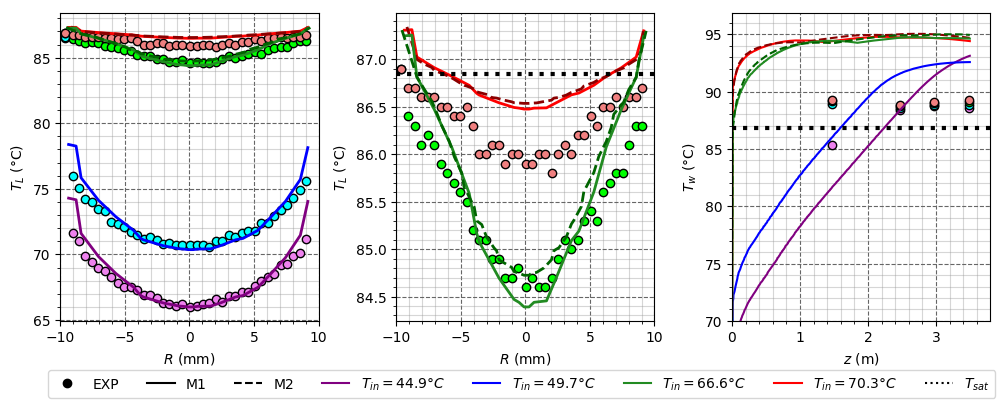
\includegraphics[scale=0.60]{img/DEBORA/c8.png}
\caption{NCFD (lines) vs. Exp. (circles) - $T_{L}$ and $T_{w}$ - Cases C8G2P26W16Te44.9, Te49.6, Te66.6 and Te70.3 - Simulations using two meshes M1 (coarse) and M2 (fine).}
\label{fig:th_1phi_res}
\end{figure}
%

%%
%\begin{figure}[!htb]
%\vspace{16pt}
%\begin{spacing}{1.0}
%\centering
%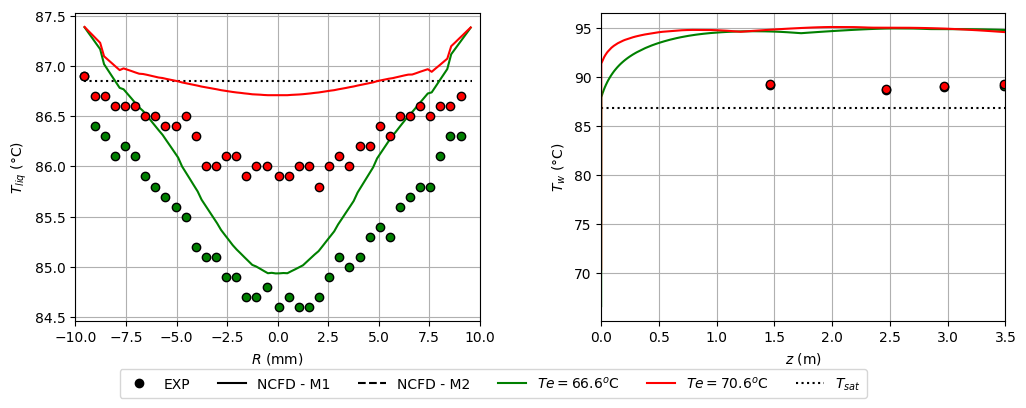
\includegraphics[scale=0.60]{img/DEBORA/thermal_diph.png}
%\caption{NEPTUNE\_CFD simulations results vs. experimental measurements - $T_{L}$ and $T_{w}$ - Cases C8G2P26W16Te66.6 and C8G2P26W16Te70.3}
%\label{fig:th_diph_res}
%\end{spacing}
%\vspace{16pt}
%\end{figure}
%%



%
\begin{figure}[h!]
\centering
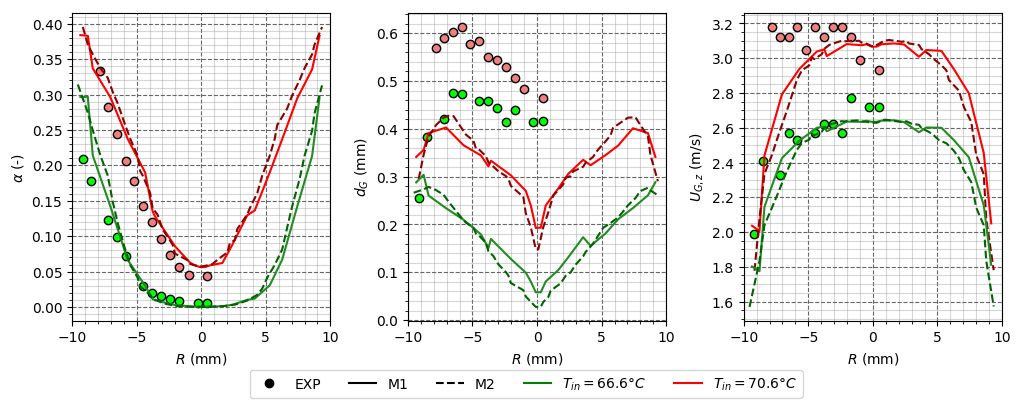
\includegraphics[scale=0.60]{img/DEBORA/c30.png}
\caption{NCFD (lines) vs. Exp. (circles) - $\alpha$, $d_{G}$ and $U_{G,z}$ - Cases C30G2P26W16Te66.6 and Te70.6 - Simulations using two meshes M1 (coarse) and M2 (fine).}
\label{fig:topology_res}
\end{figure}
%

On Figure \ref{fig:topology_res}, we compare the results of the simulations to the experiments regarding void fraction, bubble Sauter diameter and axial gas velocity. Void fraction profiles are quite correctly reproduced, though we observe a $10\%$ higher peak at the wall for $T_{in}=66.6\degree$C. The order of magnitude of bubble diameter is correct ($\sim 0.1\text{mm}$) and NEPTUNE\_CFD manages to detect coalescence (increase of bubble diameter when leaving the wall) and bulk condensation (decrease of bubble diameter when reaching the core of the flow), which is in qualitative agreement with the experiments. Quantitatively speaking, bubble diameter is globally underestimated. Finally, gas velocity profile is reasonably reproduced for $T_{in}=66.6\degree$C, but not for $T_{in}=70.6\degree$C. The latter experimental profile is flatter, which could be explained by a change of flow regime since uncondensed vapor is detected in the bulk.  

Finally, the simulations reasonably agree with the experiments. The strongest discrepancies being mostly the wall temperature and bubble diameter. Potential ways of improving those results are investigated in next sub-section.

\subsection{Investigating the nucleation site density modeling $N_{sit}$}

In NEPTUNE\_CFD, wall temperature is computed through the Heat Flux Partitioning model, which role is to find the appropriate $T_{w}$ which balances Equation $\ref{eq:HFP}$. However, some laws used to express parameters such as $N_{sit}$, $f$, or $d_{d}$ are quite old and simple. For instance, the {Lemmert} \& {Chawla}\cite{Lemmert1977} expression of $N_{sit}$ only depends on the wall superheat (Sub-section \ref{subsec:HFP}).%, meaning that it can not reproduce potential influence of the pressure on the nucleation site density.

A comparison of the {Lemmert} \& {Chawla} law\cite{Lemmert1977} with  the {Hibiki} \& {Ishii}\cite{Hibiki2003} law for $N_{sit}$ against 4 data sets from the literature is presentend on Figure \ref{fig:nsit}. The {Hibiki} \& {Ishii} correlation depends simultaneously on wall superheat, pressure and contact angle.  Experimental measurements of {Borishanskii} \etal\cite{Borishanskii1961}, {Richenderfer} \etal\cite{Richenderfer2018}, {Kossolapov} \etal\cite{Kossolapov2020} and {Zhou} \etal\cite{Zhou2020} are used to assess the two nucleation site density correlations.
%
\begin{figure}[h!]
\centering
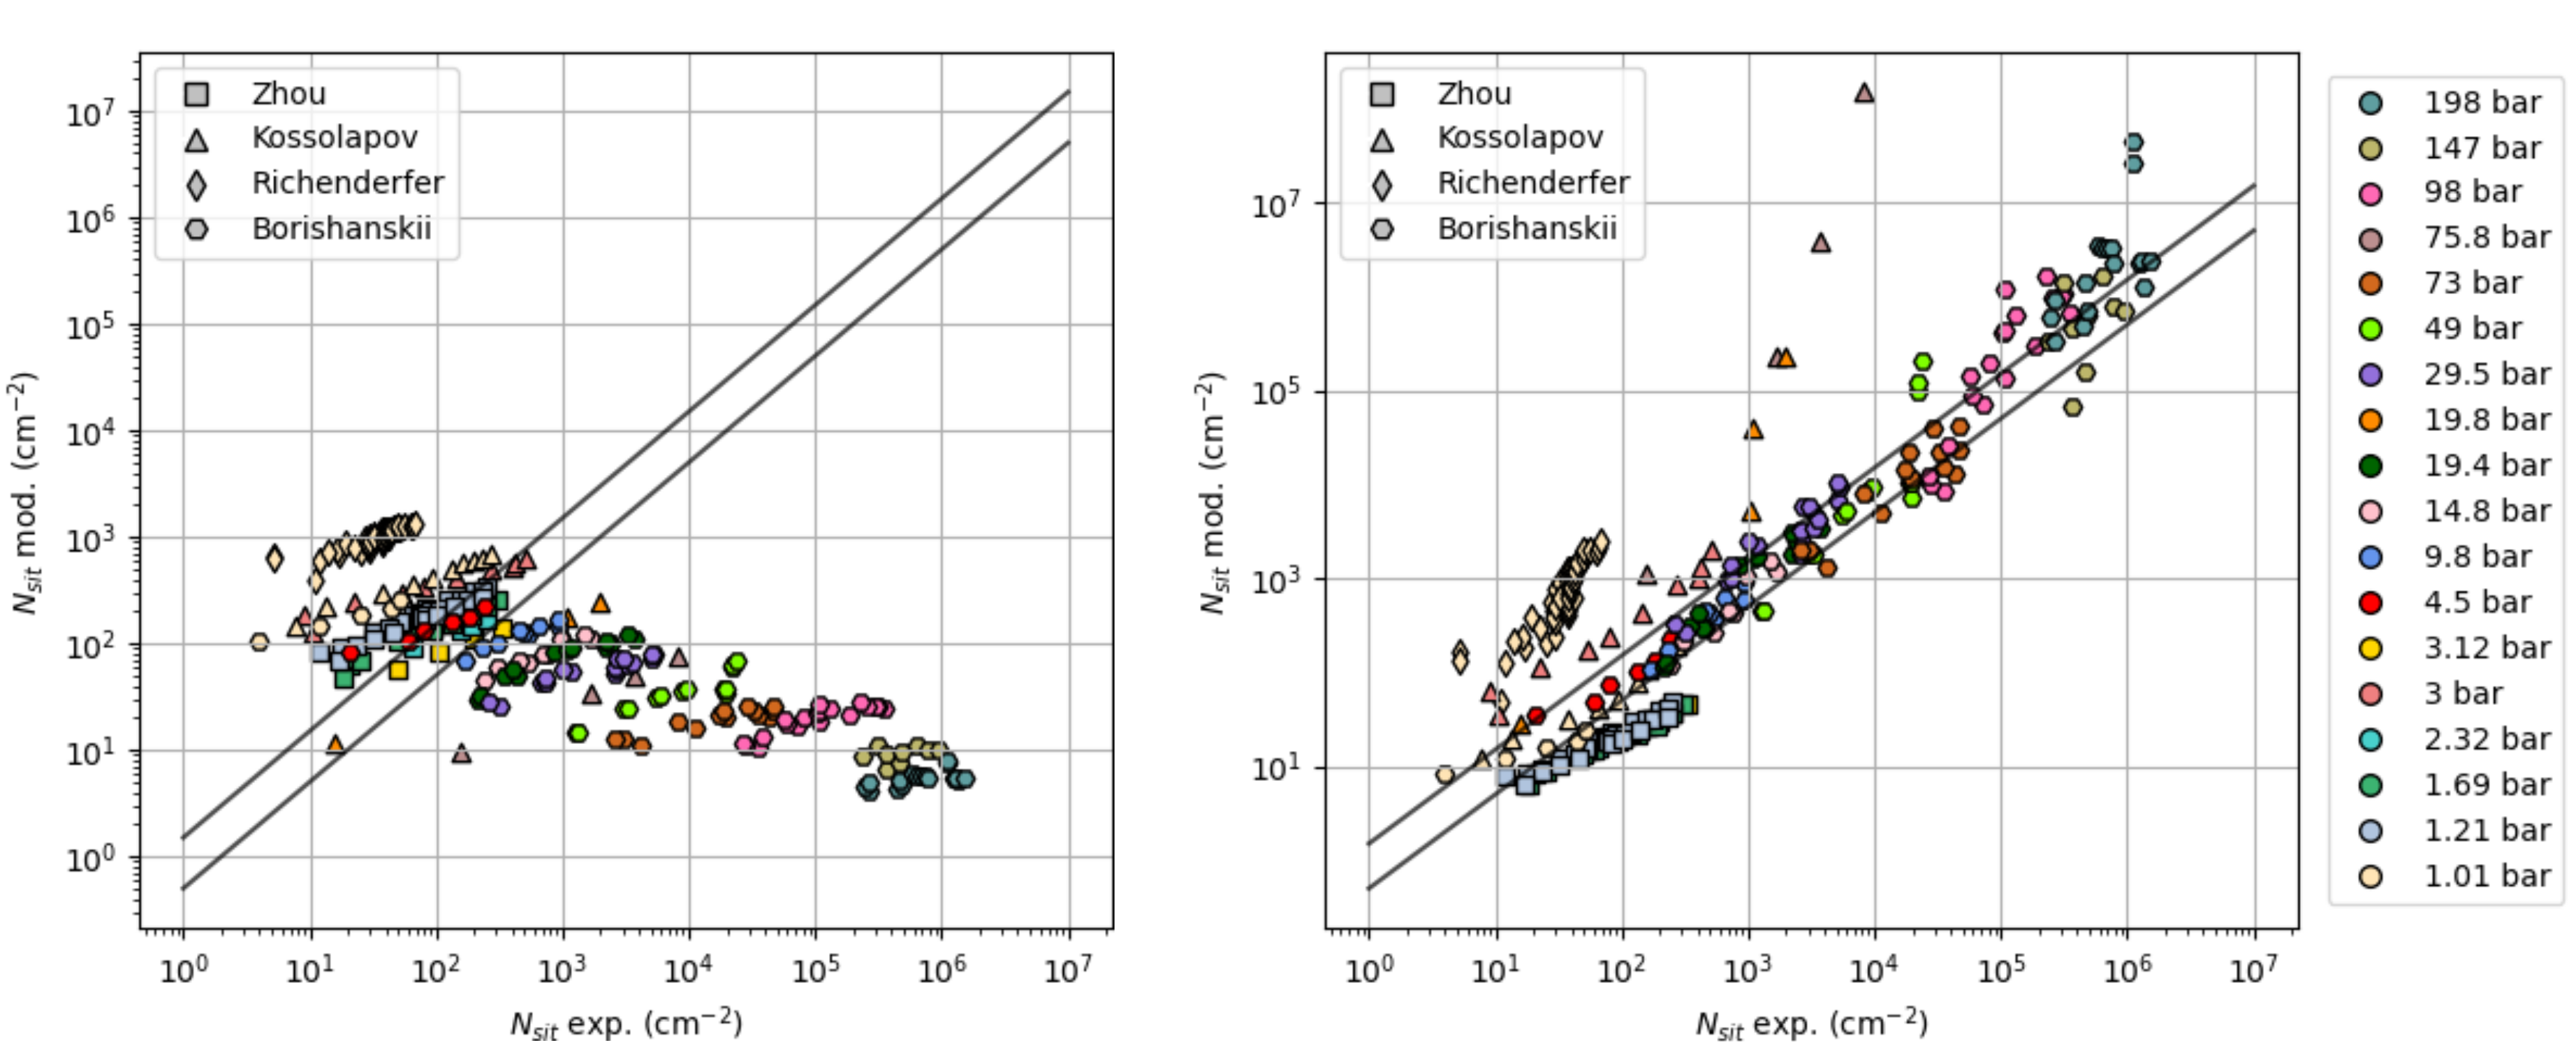
\includegraphics[scale=0.45]{img/DEBORA/nsit.png}
\caption{$N_{sit}$ correlations of {Lemmert} \& {Chawla} (left) and {Hibiki} \& {Ishii} (right) vs. exp. data from literature. Operation pressures are displayed. $\pm 50\%$ error bars are drawn in black.}
\label{fig:nsit}
\end{figure}
%

Figure \ref{fig:nsit} clearly shows that the {Lemmert} \& {Chawla} law lack of pressure dependence fails to reproduce high pressure measurements contrary to the {Hibiki} \& {Ishii} one. Even though {Hibiki} \& {Ishii} correlation shows significant discrepancies with measurements of {Kossolapov} \etal and {Richenderfer} \etal, its prediction capability is greater in average than {Lemmert} \& {Chawla} correlation.

%
\begin{figure}[h!]
\centering
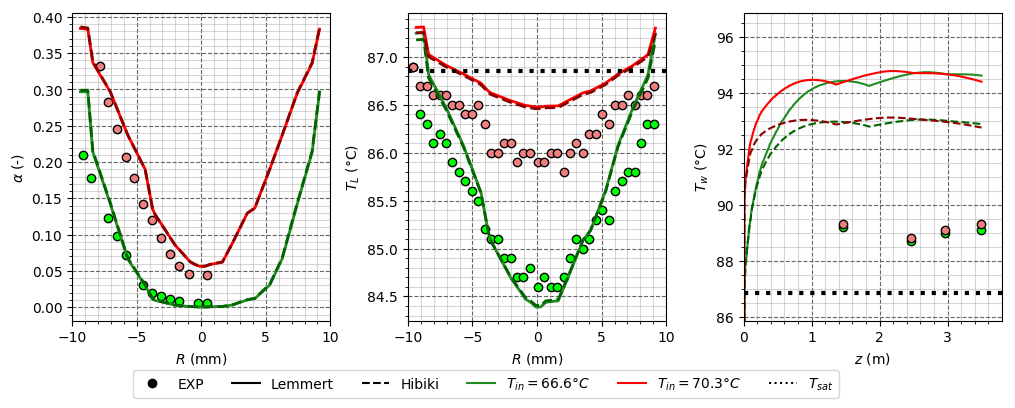
\includegraphics[scale=0.60]{img/DEBORA/plot_HI.png}
\caption{NCFD results for $\alpha$, $T_{L}$ and $T_{w}$ using {Lemmert} \& {Chawla} and {Hibiki} \& {Ishii} correlation. Cases 8G2P26W23Te66.6 and Te70.3, 30G2P26W23Te66.6 and 70.6.}
\label{fig:NCFD_nsit}
\end{figure}
%
To assess the influence of nucleation site density law on NEPTUNE\_CFD computations, we compare results obtained with both correlations on Figure \ref{fig:NCFD_nsit}, which shows a remarkable impact of the modification of $N_{sit}$ correlation. Using {Hibiki} \& {Ishii} correlation reduces the error on $T_{w}$ by approximately $2\degree\text{C}$ while $\alpha$ and $T_{L}$ remain unchanged. This implies that the same heat flux partitioning is found with the two models, but that the pressure dependence of {Hibiki} \& {Ishii} law helped to balance Equation \ref{eq:HFP} using a lower $T_{w}$, thus closer to experimental measurements.

Such a result indicates that the HFP model could be improved through a systematic analysis of each parameter's impact and modeling (bubble departure diameter, detachment frequency, etc.). Assembling a more recent and consistent model could provide better results regarding wall temperature prediction. Models such as the one developed by {Kommajosyula}\cite {Kommajosyula2020} could be interesting to apply for high-pressure flows.


Now that simple tube boiling flow has been assessed through the presented results, next section will focus on the simulation of boiling flow in a tube equipped with a mixing device.% using DEBORA-Promoteur experimental results.

\cleardoublepage % Empty page before the start of the next part


\part{Development of a New Wall Heat Flux Partitioning Model}

% Chapter X

\chapter{Existing Heat Flux Partitioning Models} % Chapter title

\label{ch:name} % For referencing the chapter elsewhere, use \autoref{ch:name} 

%----------------------------------------------------------------------------------------

\section{Kurul \& Podowski (1990)}


In their original work published in 1990, Kurul \& Podowski proposed a first complete closure for the wall heat flux partition.


\npar
They considered the applied heat flux to be divided between three mechanisms :

\begin{itemize}
\item A liquid single-phase heat flux $\phi_{c,l}$ ;
\item A boiling heat flux $\phi_{e}$ to represent phase change from liquid to vapor ;
\item A quenching heat flux $\phi_{q}$ to represent the effect of a bubble leaving the wall and being replaced by cold liquid.
\end{itemize}

The total wall heat flux being thus expressed as :

\begin{align}
\phi_{w}=\phi_{c,l}+\phi_{e}+\phi_{q}
\end{align}

Each flux being expressed as follows : 

\begin{align}
\phi_{c,l}=A_{c,l} \rho_{l} c_{p,l}U_{l,\delta} \St_{l,\delta}\parth{T_{w}-T_{l,\delta}}\\
\label{eq:phie_KP}
\phi_{e}=\frac{1}{6}\pi {D_{b}}^{3}\rho_{v}h_{lv}fN_{sit}\\
\phi_{q}=t_{q}fA_{q}\frac{2\lambda_{l}\parth{T_{w}-T_{l,\delta}}}{\sqrt{\pi \eta_{l} t_{q}}}
\end{align}

%------------------------------------------------

\subsection{Basu (2000)}

Content

%------------------------------------------------

\subsection{Yeoh (2006)}

Content

%----------------------------------------------------------------------------------------

\section{Gilman (2017)}

Content

\section{Kommajosyula (2020)}



% Chapter X

\chapter{Boiling Bubble Dynamics} % Chapter title

\label{ch:name} % For referencing the chapter elsewhere, use \autoref{ch:name} 

%----------------------------------------------------------------------------------------



\section{Force Balance Modeling}\label{sec:forces}

\subsection{General Considerations}\label{subsec:general}

When trying to derive the force balance over a bubble, the first step consists of splitting the whole effort exprienced by the bubble between different contributions depending on their nature. In our case, we focus on a bubble growing on a vertical wall and facing an upward flow as depicted in Figure \ref{fig:bub_forces}. The considered forces are :



\begin{itemize}
\item The sum of the Buoyancy and Body forces $\vect{F_{B}}$ ;
\item The Capillary or Surface Tension force $\vect{F_{C}}$ ;
\item The Contact Pressure force $\vect{F_{CP}}$ ;
\item The Drag and Lift forces $\vect{F_{D}}$ and $\vect{F_{L}}$ ;
\item The Added-Mass force $\vect{F_{AM}}$.
\end{itemize}


Regarding the bubble shape, we consider a quasi-spherical bubble of radius $R$ with a circular contact area with the wall of radius $r_{w}$. It has a static contact angle $\theta$ and is tilted under the influence of the flow by an inclination angle $\dtheta$ (half the total angle hysteresis). The resulting downstream and upstream contact angles are therefore $\theta_{d}=\theta-\dtheta$ and $\theta_{u}=\theta+\dtheta$. If the bubble has a shape close to a truncated sphere, we can to approximate the bubble foot radius as :

\begin{equation}
r_{w}\approx \frac{1}{2} R\parth{\sin{\theta_{u}} + \sin{\theta_{d}} }=R~\sin{\theta}\cos{\dtheta}
\end{equation}

We suppose $V_{b}\approx\frac{4}{3}\pi R^{3}$ for the bubble volume.

\subsection{Buoyancy and Body Forces}

The sum of the Buoyancy and Body forces results from both the weight of the bubble and the integration of the static liquid pressure over its surface which naturally yields :
\begin{equation}
\label{eq:buoyancy}
\vect{F_{B}}=V_{b}\parth{\rho_{V}-\rho_{L}}\vect{g}=\frac{4}{3}\pi R^{3}\parth{\rho_{L}-\rho_{V}}g \ \vect{e_{x}}
\end{equation}

\subsection{Capillary Force}\label{subsec:FC}

The most common and generally accepted expression of the capillary force has been derived by Klausner[cite Kl] by integrating the tangential effort at the triple contact line over the bubble foot radius while assuming an evolution of the contact angle from $\theta_{d}$ to $\theta_{u}$ as a polynomial expression of degree 3. This results in :

\begin{align}
\nonumber \vect{F_{C}}=&-\pi R \sigma \crocht{1.25\ \frac{2\dtheta}{\parth{\frac{\pi}{2}}^{2}-\dtheta^{2}}\sin{\theta}^{2}\cos{\dtheta}^{2}} \vect{e_{x}}\\
%
& - \pi R \sigma \crocht{2\ \sin{\theta}^{2}\frac{\sin{2\dtheta}}{2\dtheta}}\vect{e_{y}}
\end{align}
%where $\sigma$ is the surface tension and $\displaystyle r_{w}\approx R\  \frac{\sin{\theta_{u}}+\sin{\theta_{d}}}{2}=R\ \sin{\theta}\cos{\dtheta}$.
%&\int_{0}^{2\pi} r_{w} \sigma \vect{\tau} \mathrm{d}\alpha\\
%=& -1.25\ \frac{2\pi r_{w}\sigma \parth{\theta_{u} - \theta_{d}} }{\pi^{2} - \parth{\theta_{u} - \theta_{d}}^{2} }\crocht{\sin{\theta_{u}} + \sin{\theta_{d}}}\ \vect{e_{x}} +\frac{2\pi r_{w} \sigma}{\theta_{u} - \theta_{d}}\crocht{\cos{\theta_{u}} - \cos{\theta_{d}}}\ \vect{e_{y}}\\


\subsection{Contact Pressure Force}\label{subsec:FCP}

The Contact Pressure force originates from the pressure jump at the liquid-vapor interface exerted over the wall contact area and can be expressed using Laplace's equation as :
\begin{align}
\vect{F_{CP}}  \approx \frac{2\sigma}{R_{c}} \pi r_{w}^{2}\  \vect{e_{y}}
\approx \pi R \sigma\ 2\ \sin{\theta}^{2} \cos{\dtheta}^{2}\ \vect{e_{y}}
\label{eq:FCP}
\end{align}

Here, $R_{c}$ is the curvature radius of the bubble which is often assumed to be equal to $5R$[Klausner, Sugrue, Mazzocco] without specific justification. To avoid this arbitrary choice, following the hypothesis of a nearly spherical bubble shape gives $R_{c}=R$.
% apart that it helps the model to fit experimental measurements by ponderating the magnitude of the contact pressure force.

\subsection{Drag and Lift Forces}\label{subsec:FD}

The external liquid flow over the bubble induces the well-known Drag and Lift forces which are usually computed using associated coefficients $C_{D}$ and $C_{L}$ defined by :
\begin{align}
\vect{F_{D}}=&\frac{1}{2}C_{D}\rho_{L}S_{p}\parth{\vect{U_{L}}-\vect{U_{b}}} \norm{ \vect{U_{L}}-\vect{U_{b}} }\\
\vect{F_{L}}=&\frac{1}{2}C_{L}\rho_{L}S_{p}\parth{\vect{U_{L}}-\vect{U_{b}}}^{2}\ \vect{e_{y}}
\end{align}
with $S_{p}=\pi R^{2}$ the projected area of the bubble in the direction of the flow.


Traditional approaches rely on expressions of the Drag derived from the potential flow around the bubble[Duhar] or based on numerical correlations[Mei]. For instance, Mazzocco \etal [Mazzocco] use an expression of the Drag for a solid particle near a wall in a shear flow[Zeng] multplied by a correction factor to account for the difference between a particle and a bubble.

In this work, we propose to rely on the recent work of Shi \etal [Shi] who conducted Direct Numerical Simulations of a shear flow over a spherical bubble of constant radius close to a wall for bubble Reynolds number between $10^{-1}$ and $10^{3}$.

They computed the resulting Drag and Lift coefficients for each simulations and proposed correlations fitting their numerical results. The Drag coefficient is expressed as a correction of the Drag coefficient for a bubble in an unbounder uniform flow  $C_{D,U}$. The total drag is given by :

\begin{equation}
C_{D}=\parth{1+\Delta C_{D}}C_{D,U}
\end{equation}
where $\Delta C_{D}$ accounts for both the effect of the shear and the wall. 

To cover the whole range of bubble Reynolds numbers, correlations at low and high $\Re_{b}$ are smoothly connected using an exponential term.

\begin{equation}
\Delta C_{D}=\Delta C_{D,\Re_{b}=O\parth{1}}+\parth{1-e^{-0.07\Re_{b}}}\Delta C_{D,{\Re_{b}\gg 1}}
\end{equation}


Each of those correction is computed depending on $\Re_{b}$,  the non-dimensional shear rate $\Sr = \frac{\gamma 2R}{\bars{U_{rel}}}$, the non dimensional distances $L_{R} = \frac{y}{R}$ and $L_{u}= y \frac{\bars{U_{rel}}}{\nu_{L}}$  ($L_{R}=1$ being a spherical bubble laying on a wall). 


\begin{align}
\nonumber \Delta C_{D,\Re_{b}=O\parth{1}} = & \frac{1+\mathrm{tanh}\parth{0.012\Re_{b}^{0.8}} + \mathrm{tanh}\parth{0.07\Re_{b}^{0.8}}^{2}}{1+0.16L_{u}\parth{L_{u}+4}}
 \\
%
&\times \crocht{ \left(\frac{3}{8}L_{R}^{-1} + \frac{3}{64}L_{R}^{-4}\right) \left(1- \frac{3}{8}L_{R}^{-1}-\frac{3}{64}L_{R}^{-4}\right)^{-1}- \frac{1}{16}\left(L_{R}^{-2}+\frac{3}{8}L_{R}^{-3}\right)\text{Sr} }
\end{align}



\begin{align}
\nonumber \Delta C_{D,{\Re_{b}\gg 1}} =& ~0.47L_{R}^{-4}+0.0055L_{R}^{-6}\Re_{b}^{3/4} 
+0.002 \bars{\mathrm{Sr}}^{1.9} \Re_{b} \\
%
&+ 0.05 L_{R}^{-7/2} \mathrm{Sr} \Re_{b}^{1/3}
\end{align}


Figure \ref{fig:CD_shi} shows the evolution of the Drag correction $\Delta C_{D}$ against the bubble Reynolds number for different distances to the wall $L_{R}$ and two values of $\Sr$.  We can see that as the distance between the wall and the bubble increases the Drag correction logically approaches zero and that increasing the shear rate $\Sr$ increases $\Delta C_{D}$ for higher values of $\Re_{b}$.


Shi \etal [Shi] conducted DNS for wall distances down to $L_{R}=1.5$. However, Scheiff \etal[Scheiff] compared the values obtained for $L_{R}=1$ measured with Drag of bubbles sliding on a wall and observed a good agreement, which legitimates the use of this new Drag correlation by extending its application to the case of a bubble laying on a wall.

The chosen uniform drag coefficient $C_{D,U}$ is proposed by Mei \etal [Mei].

\begin{equation}
C_{D,U} = \frac{16}{\Re_{b}}\crocht{1 + \parth{\frac{8}{\Re_{b}}+ \frac{1}{2}\parth{1+\frac{3.315}{\sqrt{\Re_{b}}} }}^{-1} }
\end{equation}

\npar

Since this work focuses on the sliding, the total force balance will be studied along the $x$ axis, parallel to the wall. Thus, we do not detail the whole expression of Shi \etal for $C_{L}$. For further work, it is though interesting to mention that their expression of $C_{L}$ is based on the sum of three contributions (wall presence, shear and a coupled term) and changes sign when reaching negative values or $\Sr$ for instance.





\subsection{Added Mass Force}
\label{subsec:AM}

Added Mass effects originates from the transient behavior of the bubble dynamics being :

\begin{itemize}
\item Bubble growth ;
\item Freestream acceleration (not considered in this work) ;
\item Bubble acceleration.
\end{itemize}


In previous Mechanistic Models, different approaches were considered. In particular, some authors have chosen to rely on the Rayleigh-Plesset Equation for a growing hemispherical bubble in a quiescent flow to obtain the reaction force from the liquid, oriented perpendicularly to the wall.

\begin{equation}
\vect{F_{AM,RPE}}=- \rho_{L}\pi R^{2}\crocht{R\ddot{R}+\frac{3}{2}\dot{R}^{2}}\vect{e_{y}}
\end{equation}

Then, assuming an inclination angle $\theta_{i}$, this force is projected along the $x$ axis to obtain an Added Mass force parallel to the wall that hinders departure. The inclination angle value is often empiricial and used for data fitting[Klausner, Mazzocco]. 

\begin{equation}
\vect{F_{AM,RPE}}=- \rho_{L}\pi R^{2}\crocht{R\ddot{R}+\frac{3}{2}\dot{R}^{2}}\parth{\sin{\theta_{i}}\vect{e_{x}} + \cos{\theta_{i}}\vect{e_{y}}}
\end{equation}


This approach is questionable on different aspects. First, the RPE assumes a moving boundary in a quiescent unbounded liquid, which is physically far from the real situation of a bubble growing on a wall in a boiling flow. Moreover, the subsequent projection along the different directions regarding an unknown angle is hardly reasonable if $\theta_{i}$ is chosen arbitrarily.

%, considered for instance by Mazzocco[cite] Ren[cite] or Colombo[cite],

To tackle the Added Mass derivation in a proper way, we propose to follow the approach of Lamb[Lamb] (also presented by Milne Thomson[Milne] or Van Winjgaarden[Winjgaarden]). By solving the potential flow around a bubble and its image, we can obtain the total liquid kinetic energy $E_{L}$ that corresponds to a situation where a bubble is at a given distance from a wall represented by the line normal to the line of centers of the bubbles). 

Then, we can use Lagrange's equations to compute the resulting forces in each direction.


\begin{align}
\label{eq:Lag_x}
F_{AM,x}&=-\dpartial{}{t}\parth{\dpartial{E_{L}}{\dot{x}}}+\dpartial{E_{L}}{x}\\
\label{eq:Lag_y}
F_{AM,y}&=-\dpartial{}{t}\parth{\dpartial{E_{L}}{\dot{y}}}+\dpartial{E_{L}}{y}
\end{align}


To express the liquid kinetic energy, we can rely on the work of Van Der Geld[Van Der Geld] who derived $E_{L}$ in the case of a full or truncated spherical bubble laying on a wall and facing an uniform flow parallel to the wall of velocity $U_{L}$ (Eq. \ref{eq:EL_VdG}). If the bubble slides at a velocity $U_{b}=\dot{x}$, it sees a liquid velocity $U_{rel}=U_{L}-\dot{x}$.

\begin{align}
E_{L}=\frac{\rho_{L}V_{b}}{2}\parth{\alpha \dot{y}^{2} +\trb\dot{R}^{2}+\psi \dot{R}\dot{y} +\alpha_{2} \parth{U_{L}-\dot{x}}^{2} }
\label{eq:EL_VdG}
\end{align}
where $\alpha$, $\trb$, $\psi$ and $\alpha_{2}$ are polynomials of $R/y = 1/L_{R}$ derived by Van Der Geld for $1<R/y<2$ \ie $0.5<L_{R}<1$.



Injecting $E_{L}$ in Eq. \ref{eq:Lag_x} and \ref{eq:Lag_y} and computing the values for the sphere case ($y=R$) yields :

\begin{align}
\label{eq:AMx}
F_{AM,x}=\rho_{L}V_{b}\crocht{3C_{AM,x}\frac{\dot{R}}{R}U_{rel} - C_{AM,x}\dtime{U_{b}}}
\end{align}
with $C_{AM,x} \approx 0.636$.


\begin{align}
\label{eq:AMy}
F_{AM,y}=\rho_{L}V_{b}\crocht{-\parth{3 C_{AM,y1} + C_{AM,y2}}\frac{\dot{R}^{2}}{R}-C_{AM,y1}\ddot{R} + C_{AM,y3}\frac{U_{rel}^{2}}{R}}
\end{align}
with $C_{AM,y1} \approx 0.27$, $C_{AM,y2}\approx 0.326$ and $C_{AM,y3}\approx 8.77\times  10^{-3}$.


\npar
 
 


Parallel to the wall, the coupled term $\frac{\dot{R}}{R}U_{rel}$ in Eq. \ref{eq:AMx} \textbf{promotes detachment and sliding} of the bubble if $U_{rel}>0$ \eg if the bubble is attached to its nucleation site. This clearly contradicts the aforementioned approach where solely projecting the RPE on both axes lead to an Added-Mass term related to bubble growth that only hinders the departure by sliding. 

On the other hand, some authors[Klausner, Thorncroft, Guan] both projected the RPE to obtain an asymmetric growth term opposed to departure while also accounting for a detaching term due to the interaction between the flow induced by bubble growth and the external flow.

Moreover, Eq. \ref{eq:AMy} exhibits a term induced by the relative velocity that acts as a lift force, which seems to rarely appear in other approaches.

\npar
Here we want to insist on the importance on conducting an approach as rigorous as possible when deriving those transient aspects of the force balance. Otherwise, some terms may be missing and lead to contradictory physical conclusions. Although the proposed method has already been used in different works, we obtained revisited values of the Added Mass coefficients based on the derivation of the liquid kinetic energy by Van Der Geld.

In the spirit of avoiding to introduce extra empirical terms, we keep the Added Mass force as presented in Eq. \ref{eq:AMx} and \ref{eq:AMy}. No projection of the $y$ term along the $x$ axis to account for asymmetric bubble growth is considered for the moment.


\subsection{Force Balance Summary}\label{subsec:BdF}


On Table \ref{tab:all_BdF}, we sum up some of the mentioned force balance approaches and their models.






\subsection{Bubble Growth}\label{subsec:bub_growth}

The question of the bubble growth law during its lifetime including sliding is still an open question that aims to cover various types of heat transfer :

\begin{itemize}
\item Evaporation due to superheated liquid near the bubble base ;
\item Evaporation of a liquid microlayer trapped between the base of the bubble and the wall ;
\item Condensation on top of the bubble when it reaches subcooled liquid ;
\item Convective heat transfer due to relative velocity between the bubble and the liquid.
\end{itemize}

To our knowledge, many authors that have been tackling this issue had to consider empirical or fitted parameters when trying to exhaustively account for all the above heat transfers. For instance, Zhou[Zhou] and Yoo[Yoo] have proposed growth models that consider all the previously mentioned mechanisms. However, to fully close their mathematical model, many empirical values were used such as :

\begin{itemize}
\item The ratio between the bubble projected area and the microlayer area $C= A_{b}/A_{ML}$ ;
\item The fraction of bubble area facing subcooling liquid ;
\item Value of coefficients in the condensation law[Levenspiel].
\end{itemize}

Moreover, those models postulate the existence of a microlayer contributing to the growth while recent numerical and experimental investigations showed that the bubble may as well grow with a microlayer or in a pure contact line regime depending on the operating conditions [Urbano, Bures, Kossolapov].

In order to assess the force modeling proposed before, we choose a simpler growth law derived from heat conduction in the superheated liquid layer[Plesset]. 

\begin{equation}
R\parth{t} = K\Ja_{w} \sqrt{\eta_{L}t}
\end{equation}
where $K$ is an adjustable constant, with a value roughly around 2[Plesset, Zwick, Yun].

This type of bubble growth has been widely used, and showed good agreement with many experimental observations and is particularly valid for early growth stages or small bubbles at high pressure.


\subsection{Liquid Velocity}\label{subsec:liq_vel}

To compute the liquid velocity and shear rate at bubble center height, we use the wall law of Reichardt[Reichardt].

\begin{align}
U_{L}^{+} =& \frac{1}{\kappa}\ln{1+\kappa y^{+}} + c \parth{1-e^{-y^{+}/\chi} + \frac{y^{+}}{\chi}e^{-y^{+}/3} }\\
%
U_{L}=&U_{L}^{+}U_{\tau}
\end{align}
with $\kappa = 0.41$, $\chi = 11$ and $c=7.8$.

\begin{align}
\dpartial{U_{L}^{+}}{y^{+}} =& \frac{1}{1+\kappa y^{+}}+\frac{c}{\chi}\parth{e^{-y^{+}/\chi} + \parth{1-\frac{y^{+}}{3}}e^{-y^{+}/3}}\\
%
\dpartial{U_{L}}{y} =& \gamma = \frac{U_{\tau}^{2}}{\nu_{L}} \dpartial{U_{L}^{+}}{y^{+}}
\end{align}

The friction velocity is computed using Mac Adams correlation[MacAdams].

\begin{align}
U_{\tau} =& \sqrt{\frac{\tau_{w}}{\nu_{L}}}\\
\tau_{w} =& 0.018~ \Re_{D_{h}}^{-0.182}~ \frac{G_{L}^{2}}{\rho_{L}}
\end{align}

\section{Departure by Sliding}\label{sec:departure}

\subsection{Non-Dimensional Analysis}\label{subsec:adim_dep}

Now that the force balance has been established, we can write it parallel to the wall before bubble departure by sliding \ie $U_{b}=\dtime{U_{b}}=0$.

\begin{align}
\label{eq:sum_dep}
\nonumber - \pi R\sigma f_{C,x} + \frac{4}{3}\pi R^{3}\parth{\rho_{L}-\rho_{V}}g &+ \frac{1}{2}C_{D}\rho_{L}\pi R^{2} U_{L}^{2} \\
& + \frac{4}{3}\pi R^{3}\rho_{L}~3C_{AM,x}\frac{\dot{R}}{R}U_{L} = 0
\end{align}

\begin{equation}
 f_{C,x}=2.5\ \frac{\dtheta}{\parth{\pi/2}^{2}-\dtheta^{2}}\sin{\theta}^{2}\cos{\dtheta}^{2}
\end{equation}
with $f_{C,x} \to 0 $ if $\dtheta \to 0$.


We can note that the departure by sliding is promoted by the Buoyancy, the Drag and the Added Mass. Only the Capillary force keeps the bubble attached to its nucleation site.


\npar
Re-writing Eq. \ref{eq:sum_dep} in non-dimensional form by dividing the LHS by the Added Mass force yields :

\begin{equation}
\label{eq:adim_dep}
-\frac{1}{2}\frac{f_{C,x}}{K^{2}C_{AM,x}}\frac{1}{\Ca}\frac{\Pr_{L}}{\Ja_{w}^{2}} +  \frac{1}{3}\frac{1}{K^{2}C_{AM,x}}\frac{\Re_{b}}{\Fr}\frac{\Pr_{L}}{\Ja_{w}^{2}} + \frac{1}{8}\frac{C_{D}}{K^{2}C_{AM,x}}\Re_{b}\frac{\Pr}{\Ja_{w}^{2}} +1 =0
\end{equation}
where we have the following non-dimensional numbers :
\begin{align}
\nonumber \Re_{b} =& \frac{2RU_{L}}{\nu_{L}}\ ;\ \Fr=\frac{\rho_{L}U_{L}^{2}}{\parth{\rho_{L}-\rho_{V}}g R}\ ;\ \We=\frac{\rho_{L}U_{L}^{2}R}{\sigma}\ ; \ \Eo=\frac{\parth{\rho_{L}-\rho_{V}}g R^{2}}{\sigma}\ ;\\
%
\nonumber \Ja_{w}=&\frac{\parth{T_{w}-T_{sat}}\rho_{L} c_{P,L}}{\rho_{V} h_{LV}}\ ;\ \Pr_{L}=\frac{\nu_{L}}{\eta_{L}}\ ;\ \frac{\dot{R}}{U_{L}}=\frac{K^{2}\Ja_{w}^{2}}{\Pr \Re_{b}}\ ;\ \Ca=\frac{\mu_{L}U_{L}}{\sigma}
\end{align}
%=\Re_{b}^{2}\frac{\rho_{L}\nu_{L}^{2} }{g\parth{\rho_{L}-\rho_{V}}4R^{3}} 


Eq. \ref{eq:adim_dep} exhibits terms that can be used to compare the magnitude of each detaching forces. We can obtain the following conditions :

\begin{align}
&\text{Added Mass greater than Drag if :}\ \ \frac{\Ja_{w}^{2}}{\Pr}>\frac{1}{8}\frac{C_{D}}{C_{AM,x}}\frac{1}{K^{2}}\Re_{b} \label{eq:AMvsD}\\
&\text{Added Mass greater than Buoyancy if :}\ \  \frac{\Ja_{w}^{2}}{\Pr}>\frac{1}{3}\frac{1}{C_{AM,x}K^{2}}\frac{\Re_{b}}{\Fr} \label{eq:AMvsB}\\
&\text{Drag greater than Buoyancy if :}\ \  \Re_{b}>\frac{16}{3}\frac{1}{C_{D}}\frac{\Eo}{\Ca}=\Re_{c} \label{eq:DvsB}
\end{align}


Those boundaries can be plotted on a $\parth{\Ja_{w}^{2}/\Pr\ ;\ \Re_{b}}$ map for a given fluid and bubble diameter $D$. An example of such a map is presented on Figure \ref{fig:ND_map1}. This allows to visualize the operating conditions under which each of the detaching forces will be dominant. Logically, Buoyancy dominates for low $\Re_{b}$ regimes contrary to Drag. Added Mass dominates when values of $\Ja_{w}^{2}/\Pr_{L}$ are high \ie when bubble grows rapidly.


\subsubsection{Influence of Pressure}

On Figure \ref{fig:press_map}, we draw the dominance map for 3 different pressures and associated orders of magnitude of bubble departure diameter[Kocamustafaogullari].

The impact of pressure is mostly seen through the decrease of bubble departure diameter. As pressure increases, Buoyancy becomes less likely to dominate while Drag and Added Mass display much larger dominance zones. The competition between those two mainly relies on the competition between liquid flow velocity and wall superheat or heat flux.

 
\subsubsection{Comparison between Fluids}

 
On Figure \ref{fig:R12_PWR}, we compare the dominance zones for R12 at 26 bars and water at 155 bars. Moderately pressurized R12 (10 to 30 bars) has often been used as a simulating fluid to mimic water in PWR since it has the same density ratio and Weber number for instance.

Assuming that the conservation of Weber and Boiling numbers may lead to similar bubble departure diameters, we can observe that the boundaries between the two fluids are very close. This qualitatively indicates that R12 shall present bubble departure by sliding mechanisms similar to what happens in PWR, which could confort the confidence one may have in extrapolating the observations done using the simulating fluid to industrial applications.


\subsection{Low Pressure Data}\label{subsec:lowP_dep}

Now we want to apply this non-dimensional approach to experimental measurement in order to determine the actual departure by sliding regimes. We chose 3 low pressure data sets of bubble departure diameter measurements in vertical flow boiling of water. The test conditions are summarized on Table \ref{tab:lowP_data}.

In each case, we have measurements of the wall temperature which allows to precisely place the experimental point on the dominance map.

However, as explained before, we need a $D_{d}$ value to plot the dominance zones. Since measured $D_{d}$ vary significantly in each experiment, we draw the boundaries for the max. and min. $D_{d}$ values. Then, placing the measurements on the map leads to Figure \ref{fig:lowP_maps}.


The conclusion is pretty straightforward : a vast majority of the data points are located in the Added Mass dominance zone, meaning that\textbf{ the Added Mass force parallel to the wall is the main force triggering the departure by sliding}. Some points from Guan and Maity are between the boundaries for the min. and max. $D_{d}$, implying that for those bubbles Added Mass and Buoyancy were of similar magnitude when departure by sliding occurred.




\subsection{High Pressure Data}\label{subsec:highP_dep}

Following the same approach, we place experimental measurements at 20 bar and 40 bar from Kossolapov[Kossolapov] on the associated dominance map. Experimental conditions are summed up on Table \ref{tab:highP_data}.

Contrary to low pressure measurements, Kossolapov data do not provide wall temperature measurements associated to departure diameters. Using the information of the wall heat flux value, we estimate $\Delta T_{w}$ using Frost \& Dzakowic correlation[Frost].

\begin{equation}
\Delta T_{w} = \Pr_{L,sat} \sqrt{\frac{8 \sigma \phi_{w} T_{sat}}{\lambda_{L}\rho_{V}h_{LV}}}
\label{eq:frost}
\end{equation}
which yields superheats roughly between 1K and 2K. 

To cover the potential uncertainty about the estimation of $\Delta T_{w}$, the points on the map are drawn  with a uncertainty band from $\Ja_{w}/10$ to $10\times \Ja_{w}$.


The resulting map is presented on Figure \ref{fig:highP_map}. We can see the immediate difference with low pressure measurements : \textbf{all points are clearly in the Drag dominant zone}, even when considering a large uncertainty over $\Ja_{w}$. Points could reach the Added Mass / Drag boundary only for highest estimations of $\Ja_{w}$ at 20 bars. 

This main difference in the dynamic regime when bubble departs by sliding arises from multiple effects :

\begin{itemize}
\item The decrease of $\rho_{L}/\rho_{V}$ with pressure, thus reducing $\Ja_{w}$ and the impact of the detaching Added Mass term ;
\item The higher liquid mass fluxes in Kossolapov experiments, increasing the impact of the Drag ;
\item The decrease of $D_{d}$ with pressure, reducing the magnitude of Buoyancy.
\end{itemize}


\subsection{Departure Diameter Prediction}\label{subsec:Dd_pred}


After qualitative non-dimensional analysis of different experimental measurements, we can try to use the force balance to predict the bubble departure diameter of those data sets. 

We consider the non-dimensional force balance before departure.

\begin{equation}
C_{AM,x}K^{2} \frac{\Ja_{w}^{2}}{\Pr_{L}} + \frac{1}{3}\frac{\Re_{b}}{\Fr} + \frac{1}{8}C_{D}\Re_{b} = \frac{1}{2} \frac{f_{C,x}}{\Ca}
\end{equation}


Since we only have the capillary term hindering departure as a first approach, we can suppose that departure is reached when :

\begin{equation}
C_{AM,x}K^{2} \frac{\Ja_{w}^{2}}{\Pr_{L}} + \frac{1}{3}\frac{\Re_{b}}{\Fr} + \frac{1}{8}C_{D}\Re_{b} > \frac{1}{2} \frac{f_{C,x}}{\Ca}
\label{eq:pred_nogr}
\end{equation}
which is similar to saying that the total force balance becomes positive parallel to the wall.

\npar
Regarding the values of the contact angle and hysteresis, we use :

\begin{itemize}
\item $\theta=49.5\degree$ and $\dtheta = 41.5\degree$ for Sugrue data, which is the highest hysteresis measured in her experiments ;
\item $\theta = 52.5\degree$ and $\dtheta = 22.5\degree$ for Guan data, which is the average values observed in his work ;
\item $\theta = 45.5\degree$ and $\dtheta = 7.5\degree$ for Maity who measured the average contact angles for each bubble during its lifetime. 
\item $\theta = 23.6 \degree$ for Kossolapov data based on a picture of the bubble projected area and dry spot area at 10.5 bars, $\dtheta = 1\degree$ supposing small bubbles at high pressure are nearly not tilted.
\end{itemize}

This yields the resulting prediction on Figure \ref{fig:pred_nogr}. We have a significant dispersion of the results with strong underestimations of the bubble departure diameters, particularly at low pressure. This could be due to :

\begin{itemize}
\item An underestimation of the capillary term $f_{C,x}$ associated to contact angle measurements ;
\item An overestimation of a detaching term ;
\item A missing term hindering departure by sliding.
\end{itemize}

In the presented approach, the main unknown term would be the growth constant $K$ that controls the Added Mass term. However, we can also speculate that the stronger deformability of bubbles at low pressure may induce a resistive term that blocks the departure by sliding. 

This point has partially been discussed when deriving the Added Mass term in Subsection \ref{subsec:AM}. We pointed the fact that simpler approaches considering arbitrary tilting of the bubble to split the force resulting from RPE over both axes could be inaccurate. However, Klausner originally followed this approach to account for asymmetric growth of the bubble. If we wish to test a similar correction, we can rely on the growth terms found in the reassessed Added Mass force in Eq. \ref{eq:AMy}. \textbf{To avoid using an arbitrary inclination angle}, we use $\theta_{i}=\dtheta$ which represents the bubble tilt through its hysteresis as depicted in Figure \ref{fig:bub_forces}.

We thus add a non-dimensional term derived from the projection of the bubble growth term of Eq. \ref{eq:AMy} on the $x$ axis :

\begin{equation}
C_{AM,x}K^{2} \frac{\Ja_{w}^{2}}{\Pr_{L}} + \frac{1}{3}\frac{\Re_{b}}{\Fr} + \frac{1}{8}C_{D}\Re_{b} > \frac{1}{2} \frac{f_{C,x}}{\Ca}  + \frac{\parth{2C_{AM,y1}+C_{AM,y2}}}{3}\frac{K^{4}\Ja_{w}^{4}}{\Pr_{L}^{2} \Re_{b}}\sin{\dtheta}
\label{eq:pred_gr}
\end{equation}

This correction yields $D_{d}$ predictions of Figure \ref{fig:pred_gr}. The predictions are significantly improved for the low pressure measurements while they remain unchanged for the high pressure cases. This could be expected with the small $\Ja_{w}$ values reached.


On the other hand, both cases show nearly no variation in the predicted departure diameters for Kossolapov data. Suspecting that this originates from the very low value chosen for $\dtheta$, we try a slightly higher value of $\dtheta = 4\degree$ as a sensitivity test. 

Results on Figure \ref{fig:pred_Koss4deg} show that this higher value of $\dtheta$ permits a better prediction of high pressure measurements. Moreover, we observe no impact of using the projected growth term of Equation \ref{eq:pred_gr}.

However, Kossolapov specified in his work that defining the departure event at high pressure was complicated because of both the nearly zero Capillary force hindering departure and the fact that bubbles started to leave their nucleation site nearly instantly[Kossolapov].


Generally speaking, once we consider the projected term for low pressure measurements, the model achieves reasonable predictions and exhibits a coherent trend with pressure. Although those results may appear less precise than other existing mechanistic models[Klausner, Mazzocco], we want to insist that our approach was conducted using a reduced number of arbitrary / empirical constants. Usually, other models rely on calibrated values of $r_{w}$, $\theta_{i}$, $\dtheta$ or $K$, which helps to achieve better predictions on given data sets.



\section{Sliding phase}\label{sliding}


\subsection{Modeling}

After departure, bubbles slide over a distance $l_{sl}$ which scales the impact of the sliding phenomenon over the wall heat transfer. Achieving good prediction of bubble sliding velocity is then important if one wishes to correctly quantify its impact. 

Following the force balance framework presented in Section \ref{sec:forces}, we can write Newton's second law parallel to the wall for the sliding bubble.


\begin{align}
\nonumber \rho_{V}\derive{\parth{V_{b}U_{b}}}{t} =& - \pi R\sigma f_{C,x}+ \frac{4}{3}\pi R^{3}\parth{\rho_{L}-\rho_{V}}g + \frac{1}{2}C_{D}\rho_{L}\pi R^{2} U_{L}^{2} \\
%
&+ \frac{4}{3}\pi R^{3}\rho_{L}\crocht{3C_{AM,x}\frac{\dot{R}}{R}U_{rel} - C_{AM,x}\derive{U_{b}}{t}}
\end{align}

This equation can be re-writed to express the bubble acceleration.

\begin{align}
\nonumber \parth{1+\frac{\rho_{L}}{\rho_{V}}C_{AM,x}}\derive{U_{b}}{t} = & \parth{\frac{\rho_{L}}{\rho_{V}}-1}g + \frac{3}{8}\frac{C_{D}}{R}\frac{\rho_{L}}{\rho_{V}}\parth{U_{L}-U_{b}}\bars{U_{L}-U_{b}} \\
%
&+ 3\frac{\dot{R}}{R}\crocht{C_{AM,x}\frac{\rho_{L}}{\rho_{V}}\parth{U_{L}-U_{b}}-U_{b}} - \frac{3}{4}\frac{\sigma}{\rho_{V}}\frac{f_{C,x}}{R^{2}}
\label{eq:ub_dot}
\end{align}

Then, we numerically solve this equation from the moment when $R\geq R_{d}$ using a first order Euler scheme. Next sections compare obtained results against low and high pressure data.


\subsection{Low Pressure Sliding}

Maity[Maity] provided simultaneous measurements of bubble radius and velocity over time for three liquid mass fluxes in vertical boiling. To assess the validity of Eq. \ref{eq:ub_dot}, we modify the growth constant $K$ in order to roughly match experimental radius measurements. The goal is to verify if the force balance allows a good prediction of bubble velocity provided a correct bubble growth. The contact angles were kept the same as in \ref{subsec:Dd_pred} since Maity provided average values over the bubble lifetime.

Results are displayed on Figure \ref{fig:slide_maity}. The model seems to fairly good predict bubble sliding velocity for the 3 cases. The moment of departure is a bit underestimated as previously observed (Figure \ref{fig:pred_gr}).

The biggest discrepancy is observed for the case at $G_{L}=143.8~ \debm$. The slope of the velocity profile is close to the experiments, but the bubble reaches a nearly constant acceleration too rapidly which yields an approximately constant overestimation of $0.1$~m/s.

The $G_{L}=239.6~ \debm$ is well predicted regarding the velocity. However, the growth profile was difficult to match since measurements exhibit significant changes in growth regime after departure, which is probably due to the bubble being large enough to be impacted by the bulk flow. A finer model for bubble growth could be of interest here.


We can note that values of $K$ between 0.5 and 1 were used to better fit the bubble radius time profile.



\subsection{High Pressure}

In his work, Kossolapov conducted measurements of radius and sliding length over thousands of individual bubbles and then provided the associated statistical distributions. To compare our model with his measurements, we took the upper and lower bounds of $R$ and $l_{sl}$ over time and plotted the associated bands of measured values as shown on Figure \ref{fig:slide_koss_20bar} and \ref{fig:slide_koss_40bar}.


Comparisons were done for cases at 20 bar and 40 bar and 3 different values of $G_{L}$. The value of $\dtheta$ for the simulations was kept really small ($2 \degree$ at 20 bar and $0.5\degree$ at 40 bar) since bubble tilt is supposed to reduce during sliding because the relative velocity regarding the liquid flow is diminishing. Moreover, higher pressure means smaller bubbles that are even more unlikely to present a significant contact angle hysteresis. We also want to mention that neglecting the capillary term in Eq. \ref{eq:ub_dot} had a minor impact over the results except that the bubble accelerates a little bit faster. 

The obtained results are in good agreement both with the observed values of sliding length its evolution, which means bubble sliding velocity is well predicted for theses cases.

On the other hand, we must note that high values of $K$ were needed to match bubble growth measurements. This may be due to an underestimation of the wall superheat coming from Eq. \ref{eq:frost}.



\section{Conclusion}\label{ccl}

In this work, we proposed a revisited force balance for a single bubble in an vertical upward boiling flow. A recent correlation for the Drag coefficient was used thanks to DNS results of Shi \etal and new values of the Added Mass coefficients were derived from the expression of the liquid kinetic energy in a potential flow around a bubble proposed by Van Der Geld.

This force balance also uses a limited amount of empirical variables to avoid data fitting and try to rely as much as possible on the derived expressions.

From this modeling, a non-dimensional approach was conducted to study the departure by sliding process and identify the main detaching forces at the moment of departure. A non-dimensional map was used to determine the operating conditions ranges for which each force is dominant. Using experimental measurements of bubble departure diameter, it was found that Added Mass was the main detaching force at low pressure while high pressure departure by sliding is dominated by the Drag.

This force balance was then used to predict bubble departure diameter values. A global underestimation was found which could be corrected at low pressure by including a bubble inclination term that partially projects the orthogonal Added Mass force associated to growth along the wall. The lack of precision compared to other existing models is likely due to the absence of fitting parameters such as the bubble foot radius, inclination angle or growth rate. However, the model showed an acceptable trend with pressure which can be considered as an encouraging feature regarding its generality.

Finally, bubble sliding simulations were conducted and compared with low and high pressure data. The results showed great agreement with measurements if an appropriate bubble growth is used. This indicates that the proposed modeling of the forces correctly captures the dynamics of sliding bubbles.

\npar

Further work shall be conducted on a clean modeling of the bubble growth by including effects such as condensation, microlayer evaporation and impact of the external liquid flow. Existing models rely on many empirical values which thus reduces their general applicability outside of their validation range. For instance, studies conducted by Zhou[Zhou] and Yoo[Yoo] could be used by enriching their modeling with finer results to get rid of data fitting. DNS results such as those of Legendre \etal [Legendre] could be of interest in that prospect.

Finally, the precise estimation of the contact angle and hysteresis remains a critical parameter to predict departure by sliding. Local measurements of those values and their evolution with operating conditions would be a very valuable information in that regard. 





\begin{figure}[h!]
\centering

\fbox{


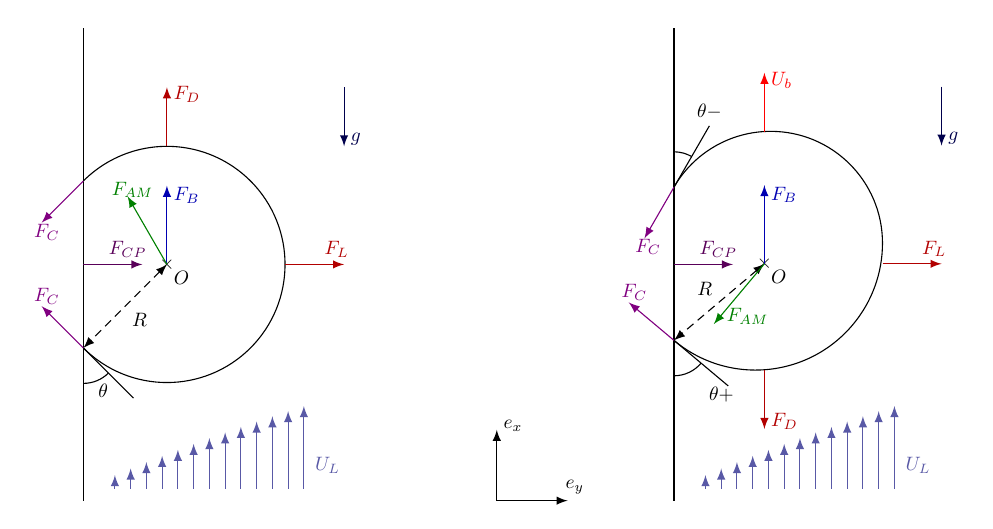
\begin{tikzpicture}[scale=3.0, every node/.style={scale=0.7}]


%%%Truncated sphere on a vertical wall

\coordinate (O1) at (0,0);
\coordinate (O2) at (0,2);

\draw (O1)--(O2);

\coordinate (Ob) at (0,1.0);

\tikzmath{\thet = 45; \thetrad= \thet * pi / 180; \ray=0.5; \rw=\ray * sin(\thetrad r);};


\coordinate (Oarc) at ($(Ob)-(0,{\ray * sin(\thetrad r)})$);
\draw (Oarc) arc({(-pi+\thetrad ) r}:{(pi-\thetrad ) r}:\ray);

%Upstream angle
\draw (Oarc) --++(-90+\thet:0.3);
\draw ($(Oarc)+(0,-0.15)$) arc(-90:-90+\thet:0.15) node[near end, below]{$\theta$};

%%Downstream angle
%\coordinate (Oarc2) at ($(Oarc) - (2*\rw,0)$);
%\draw (Oarc2) --++(180-\thet:0.3);
%\draw ($(Oarc2)+(-0.15,0)$) arc(180:180-\thet:0.15) node[near end, left]{$\alpha$};

%Center and radius

\coordinate (Cb) at ($(Ob)+({\ray*cos(\thetrad r)},0 )$);
\draw (Cb) node{$\times$} node[below right]{$O$};

\draw[densely dashed, <->, >=latex] (Cb) -- (Oarc) node[midway, below right]{$R$};


%%Forces

\draw[->, >=latex, violet!70!black] (Ob)--++(\ray/2,0) node[near end, above]{$\vect{F_{CP}}$};

\draw[->, >=latex, red!70!black!] ($(Cb)+(\ray,0)$)--++(\ray/2,0) node[very near end, above]{$\vect{F_{L}}$};
\draw[->, >=latex, red!70!black!] ($(Cb)+(0,\ray)$)--++(0,\ray/2) node[very near end, right]{$\vect{F_{D}}$};

\coordinate (Oarc2) at ($(Oarc)+(0,{2*\rw})$);
\draw[->, >=latex, violet] (Oarc)--++(90+\thet:\ray/2) node[very near end, above]{$\vect{F_{C}}$};
\draw[->, >=latex, violet] (Oarc2)--++(-90-\thet:\ray/2) node[very near end, below]{$\vect{F_{C}}$};

\draw[->, >=latex, blue!70!black] (Cb)--++(0,\ray/1.5) node[very near end, right]{$\vect{F_{B}}$};


\draw[->, >=latex, green!50!black!] (Cb)--++(90+\thet/1.5:\ray/1.5) node[very near end, above]{$\vect{F_{AM}}$};

%Gravity

\draw[->, >=latex, blue!30!black]  ($(Cb)+({1.5*\ray},{1.5*\ray})$)--++(0,-\ray/2) node[very near end, right]{$\vect{g}$};


%Flow arrows
\foreach \i in {2,...,14} 
{
\coordinate (Oloc) at ($(O1)+(\i/15,0.05)$);
\draw[->,>=latex, gray!70!blue] (Oloc)--++(0,{ln(1+0.03*\i)});
}
\draw[gray!70!blue] ($(Oloc)+(0.1,0.1)$) node{$\vect{U_{L}}$};

%Referential vectors
\coordinate (Ovect) at (1.75,0);
\draw[->, >=latex] (Ovect)--++(0.3,0) node[very near end, above right]{$\vect{e_{y}}$};
\draw[->, >=latex] (Ovect)--++(0,0.3) node[very near end, above right]{$\vect{e_{x}}$};




%Tilted bubble
\coordinate (Ob2) at (2.5,1.0);

\coordinate (O1) at (2.5,0);
\coordinate (O2) at (2.5,2);
\draw (O1)--(O2);

\tikzmath{\thet = 40; \thetrad= \thet * pi / 180;
\dthet=10; \dthetrad=\dthet*pi/180;
\thetadvrad=\thetrad - \dthetrad;
\thetrecrad=\thetrad + \dthetrad;
\thetadv=\thetadvrad*180/pi;
\thetrec=\thetrecrad*180/pi;
\ray=0.5; 
\rayadv=\ray *(1+cos(\thetrad r))/(1+ cos(\thetadvrad r);
\rayrec=\ray *(1+cos(\thetrad r))/(1+ cos(\thetrecrad r);};

\coordinate (Oarc) at ($(Ob2)-(0,{\ray * sin(\thetrad r)})$);


\draw (Oarc) arc({-pi+(\thetrecrad)) r}:{0 r}:\rayrec) arc ({0 r}:{pi-(\thetadvrad)) r}:\rayadv);

%Upstream angle
\draw (Oarc) --++(-90+\thetrecrad r:0.3) node[very near end, below]{$\theta + \dtheta$};
\draw ($(Oarc)+(0,-0.15)$) arc(-90:-90+\thetrecrad r:0.15) ;

%Downstream angle
\coordinate (Oarc2) at ($(Oarc) + (0,{\rayadv * sin(\thetadvrad r) + \rayrec * sin(\thetrecrad r)})$);
\draw (Oarc2) --++({90-(\thetadvrad r)}:0.3);
\coordinate (angadv) at ($(Oarc2) +({90-(\thetadvrad r)}:0.3)$);
\draw (angadv)  node[above]{$\theta - \dtheta $};
\draw ($(Oarc2)+(0,+0.15)$) arc(90:{90-(\thetadvrad r)}:0.15);



%Center and radius

\coordinate (Cb) at ($(Oarc2)+( {\ray * cos(\thetrad r)} , {-0.5 * (\rayadv * sin(\thetadvrad r) + \rayrec  * sin(\thetrecrad r) )})$);
\draw (Cb) node{$\times$} node[below right]{$O$};

\draw[densely dashed, <->, >=latex] (Cb) -- (Oarc) node[midway, above left]{$R$};


%Inclination angle

%\draw[densely dotted] (Cb) --++ (0.7,0);
%\draw[densely dotted] (Cb) --++ ({(1*\dthetrad r)}: 0.7 );
%\draw ($(Cb) + (0.3,0)$) arc(0: {(\dthetrad r)}:0.3)  node[midway, right]{$\dtheta$};
%
%



%%Forces

\draw[->, >=latex, violet!70!black] (Ob2)--++(\ray/2,0) node[near end, above]{$\vect{F_{CP}}$};

\draw[->, >=latex, red!70!black!] ($(Cb)+(\ray,0)$)--++(\ray/2,0) node[very near end, above]{$\vect{F_{L}}$};
\draw[->, >=latex, red!70!black!] ($(Cb)+(0,-\rayadv*0.95)$)--++(0,-\ray/2) node[very near end, right]{$\vect{F_{D}}$};
\draw[->, >=latex, red] ($(Cb)+(0,+\rayrec*1.04)$)--++(0,+\ray/2) node[very near end, right]{$\vect{U_{b}}$};


\draw[->, >=latex, violet] (Oarc)--++(90+\thetrec:\ray/2) node[very near end, above]{$\vect{F_{C}}$};
\draw[->, >=latex, violet] (Oarc2)--++(-90-\thetadv:\ray/2) node[very near end, below]{$\vect{F_{C}}$};

\draw[->, >=latex, blue!70!black] (Cb)--++(0,\ray/1.5) node[very near end, right]{$\vect{F_{B}}$};


\draw[->, >=latex, green!50!black!] (Cb)--++(90-\thet:-\ray/1.5) node[very near end, right]{$\vect{F_{AM}}$};

%Gravity

\draw[->, >=latex, blue!30!black]  ($(Cb)+({1.5*\ray},{1.5*\ray})$)--++(0,-\ray/2) node[very near end, right]{$\vect{g}$};



%Flow arrows
\foreach \i in {2,...,14} 
{
\coordinate (Oloc) at ($(O1)+(\i/15,0.05)$);
\draw[->,>=latex, gray!70!blue] (Oloc)--++(0,{ln(1+0.03*\i)});
}
\draw[gray!70!blue] ($(Oloc)+(0.1,0.1)$) node{$\vect{U_{L}}$};



\end{tikzpicture}

}

\caption{Sketch of the forces applied to the bubble facing an upward flow $\vect{U_{L}}$ and sliding at velocity $\vect{U_{b}}$}
\label{fig:bub_forces}
\end{figure}
 



\begin{figure}[h!]
\centering
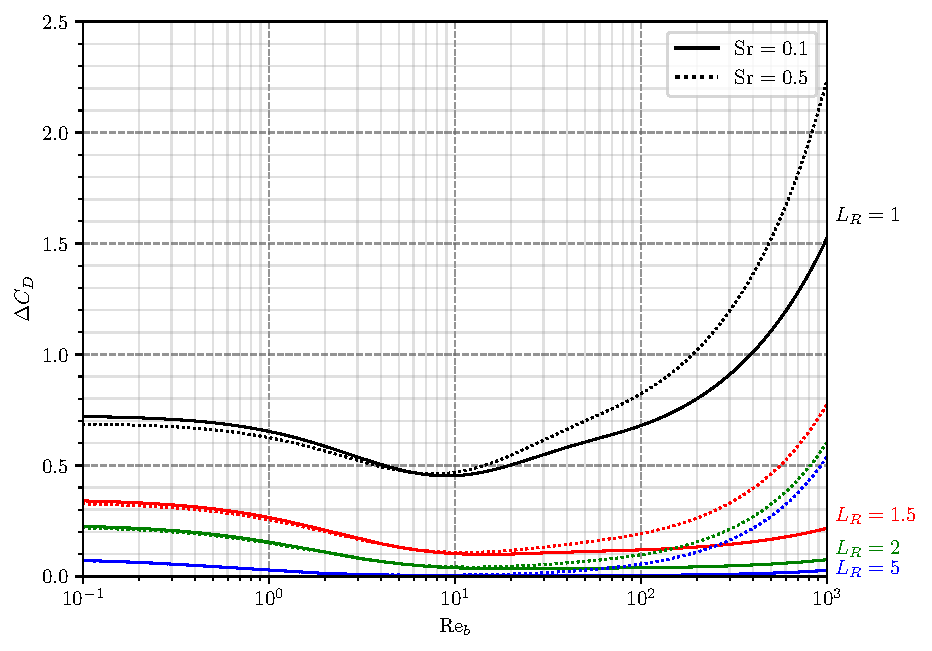
\includegraphics[width=0.8\linewidth]{img/forces/corr_drag.pdf}
\caption{Drag correction from Shi \etal [Shi].}
\label{fig:CD_shi}
\end{figure}





\begin{table}[H]
\scriptsize
\centering
\begin{center}
{\setlength{\tabcolsep}{7pt}
{\renewcommand{\arraystretch}{1.5}
\begin{tabular}{|p{2mm}|p{6mm}|p{17mm}|p{17mm}|p{17mm}|p{17mm}|p{17mm}|p{17mm}|}
\hline 
 & & \multicolumn{6}{|c|}{Authors} \\
\hline
 & & Klausner & Thorncroft & Sugrue & Mazzocco & Ren & Present \\
\hline
\multirow{6}*{\rotatebox{90}{Forces}} &  $\vect{F_{B}}$ & Eq. \ref{eq:buoyancy} & Eq. \ref{eq:buoyancy} & Eq. \ref{eq:buoyancy} & Eq. \ref{eq:buoyancy} & Eq. \ref{eq:buoyancy} & Eq. \ref{eq:buoyancy} \\
   %\cline{2-4}
& $\vect{F_{C}}$ & [Klausner] & [Klausner] & [Klausner] & [Klausner] & [Klausner] & [Klausner]  \\
  %\cline{2-4}  
& $\vect{F_{CP}}$ & Eq. \ref{eq:FCP} &  Eq. \ref{eq:FCP} &  Eq. \ref{eq:FCP} &  Eq. \ref{eq:FCP} & Eq. \ref{eq:FCP} & Eq. \ref{eq:FCP}  \\
 %\cline{2-4}
& $\vect{F_{D}}$ & [Mei] & [Mei] & [Mei] & [Zeng] $\times $ 0.66 & [Mei] & [Shi] + [Mei]  \\
& $\vect{F_{L}}$ & a & a & a & a & a & [Shi]  \\
& \multirow{3}*{$\vect{F_{AM}}$} & {RPE,\newline $\theta_{i}=\pi/17$} & {RPE,\newline $\theta_{i}=\pi/17$} & {RPE,\newline $\theta_{i}=\pi/17$} & {RPE, $\cos{\theta_{i}}=1$, $\sin{\theta_{i}}=0.2$ }& {RPE,\newline $\theta_{i}=\pi/17$} & {Potential flow [VdG] \newline + Lagrange equation} \\
\hline
\end{tabular}}}
\label{BdF_summ}
\caption{Summary of different force-balance mechanistic approaches}
\label{tab:all_BdF}
\end{center}
\end{table}




\begin{figure}[h!]
\centering
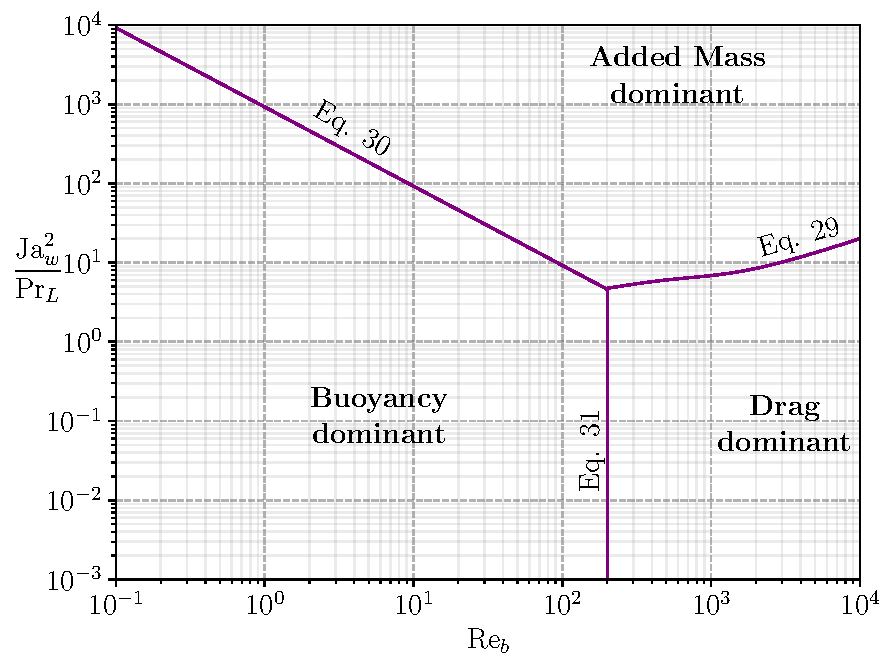
\includegraphics[width=1.0\linewidth]{img/forces/ND_map1.pdf}
\caption{Dominance map regarding departure by sliding. Boundaries plotted for water at 1 bar and $D_{d}=0.5$mm.}
\label{fig:ND_map1}
\end{figure}





\begin{figure}[h!]
\centering
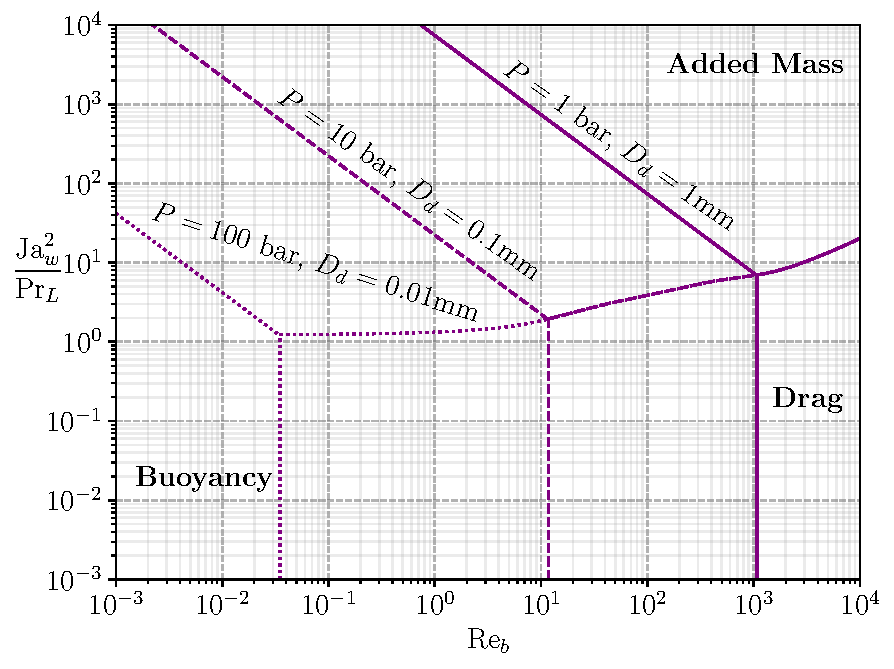
\includegraphics[width=1.0\textwidth]{img/forces/press_map.pdf}
\caption{Dominance map plotted for water at different pressures and bubble departure diameters.}
\label{fig:press_map}
\end{figure}





\begin{figure}[h!]
\centering
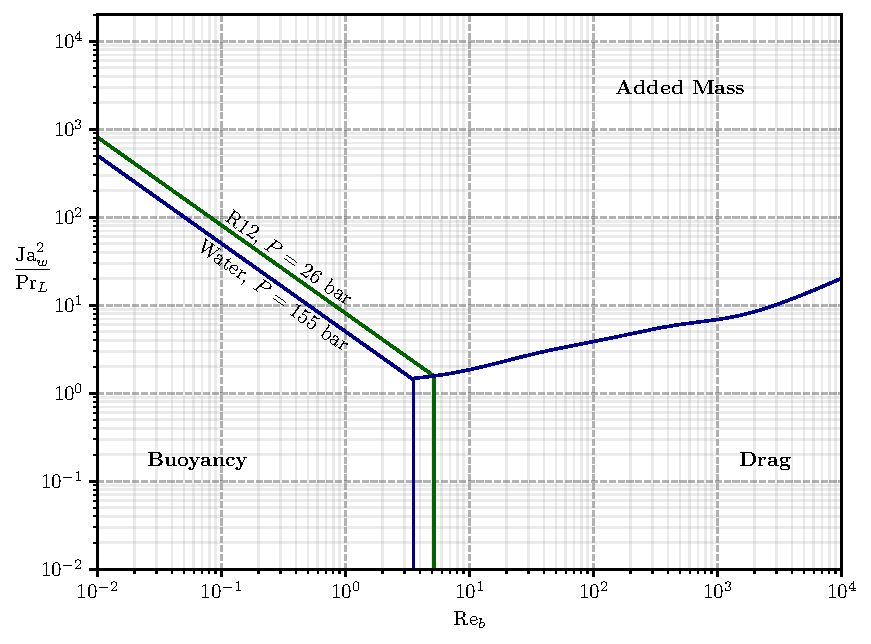
\includegraphics[width=1.0\linewidth]{img/forces/R12_PWR.pdf}
\caption{Dominance map for R12 as simulating fluid for PWR. $D_{d}=0.05$mm is chosen according to R12 measurements from Garnier \etal[Garnier] who found bubbles of $\sim 0.1$mm diameter after lift-off.}
\label{fig:R12_PWR}
\end{figure}






\begin{table}[h!]
\scriptsize
\centering
\begin{tabular}{|c||c|c|c|c||c|c|} \hline
Author &  $D_{h}$ [mm] & $G_{L}$ [$\debm$] & $\Delta T_{w}$ [K] & $D_{d}$ [mm]  & $\Re_{b}$ (-) & $\Ja_{w}^{2}/\Pr$ (-)\\
\hline
\hline
Sugrue \etal[Sugrue] & 16.642 & 250 - 400 & 2 - 6 & 0.229 - 0.391 & 139.1 - 180.1 & 20.57 - 185.2 \\
\hline
Guan \etal[Guan] & 9 & 87.3 - 319.2 & 4.5 - 8.5 & 0.62 - 1.85 & 193.3 - 923.4& 104.2 - 371.6 \\
\hline
Maity[Maity] & 20 & 0 - 239.6 & 5 - 5.9 & 0.788 - 1.713 & 186.6 - 516.7 & 128.6 - 179.06 \\
\hline
\end{tabular}
\caption{Thermal-hydraulics parameters range for the low pressure data.}
\label{tab:lowP_data}
\end{table}




\begin{figure}[h!]
\begin{center}
\subfloat[Sugrue data]{
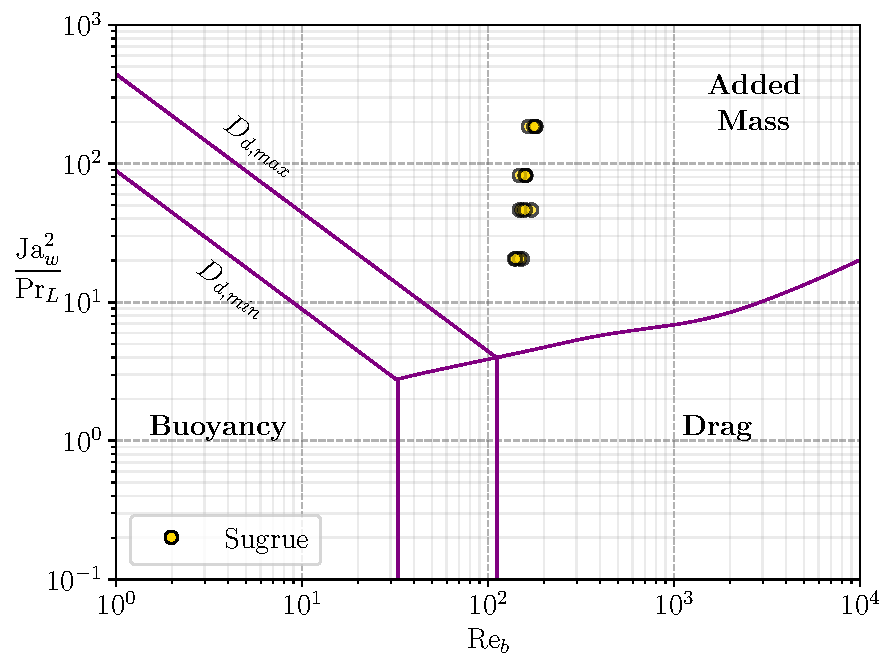
\includegraphics[width=0.5\linewidth]{img/forces/sugrue.pdf}
} 
\subfloat[Guan data]{
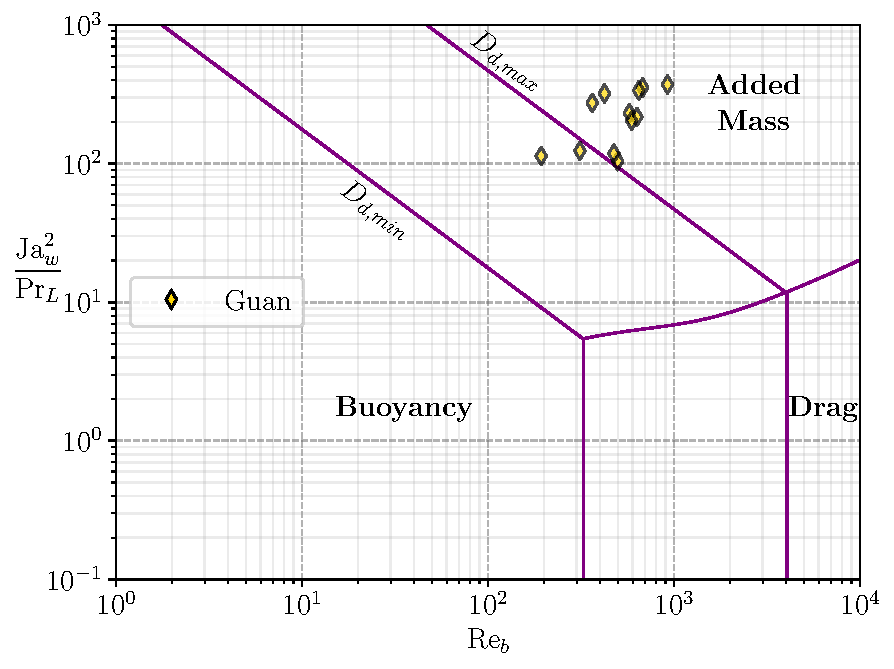
\includegraphics[width=0.5\linewidth]{img/forces/guan.pdf}
}
\\
\subfloat[Maity data]{
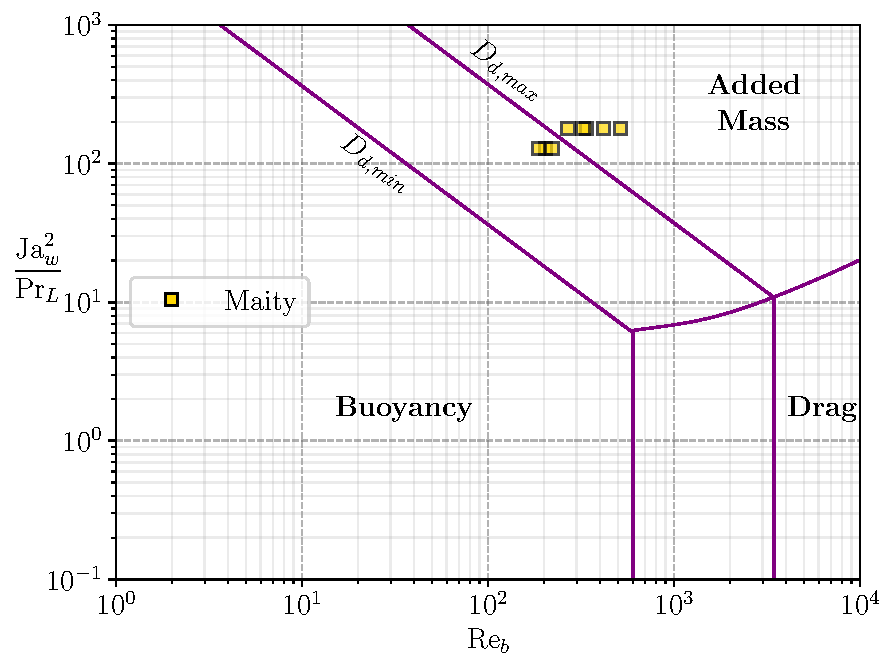
\includegraphics[width=0.5\linewidth]{img/forces/maity.pdf}
}

	\caption{Dominance maps for each low pressure data sets.}	
	\label{fig:lowP_maps}
\end{center}
\end{figure}






\begin{table}[h!]
\scriptsize
\centering
\begin{tabular}{|c||c|c|c|c|c||c|} \hline
Author &  $D_{h}$ [mm] & $G_{L}$ [$\debm$] & $P$ [Bar]  & $\phi_{w}$ [MW.m\up{-2}] & $D_{d}$ [mm]  & $\Re_{b}$ [-] \\
\hline
\hline
\multirow{2}*{Kossolapov[Kossolapov]} & \multirow{2}*{11.78} &  \multirow{2}*{500-1500} & 19.9 & 0.178 - 0.495 & 0.021 - 0.047 & 43.9 - 110.2\\
 &  &  &  39.8  & 0.291 - 0.613 & 0.01 - 0.035 & 17.0 - 55.9\\
\hline
\end{tabular}
\caption{Thermal-hydraulics parameters range for Kossolapov data.}
\label{tab:highP_data}
\end{table}





\begin{figure*}[h!]
\centering
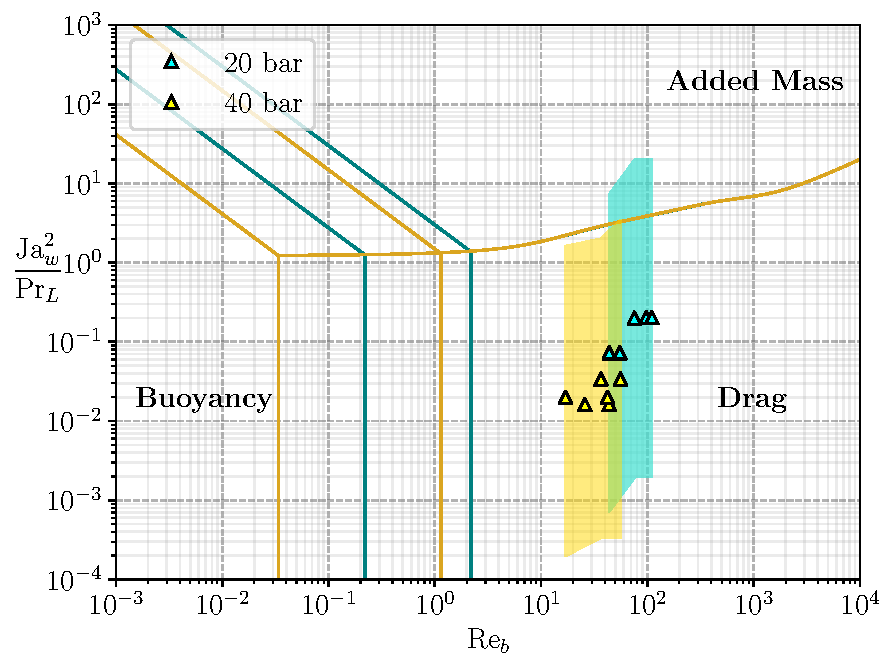
\includegraphics[width=0.7\textwidth]{img/forces/kossmap_all.pdf}
\caption{Dominance map for high pressure measurements from Kossolapov}
\label{fig:highP_map}
\end{figure*}




\begin{figure*}[h!]
\centering
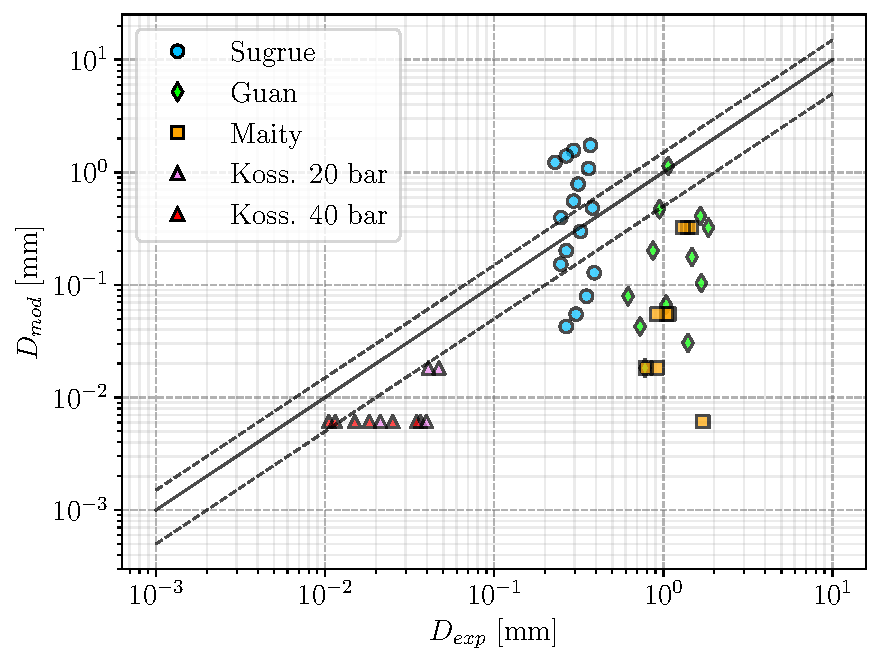
\includegraphics[width=0.7\textwidth]{img/forces/pred_nogr.pdf}
\caption{$D_{d}$ predictions using Eq. \ref{eq:pred_nogr}}
\label{fig:pred_nogr}
\end{figure*}




\begin{figure*}[h!]
\centering
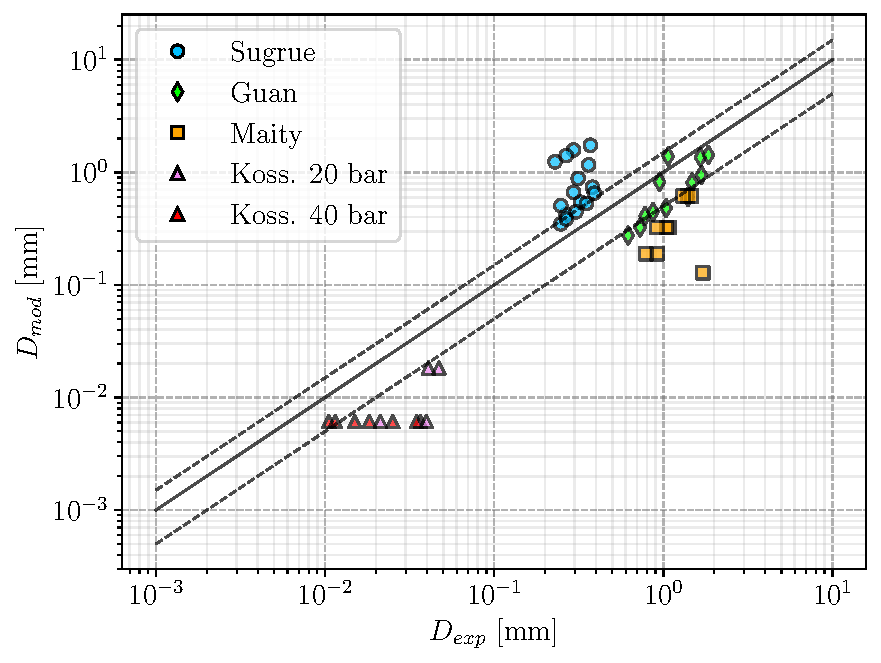
\includegraphics[width=0.7\textwidth]{img/forces/pred_gr.pdf}
\caption{$D_{d}$ predictions using Eq. \ref{eq:pred_gr}}
\label{fig:pred_gr}
\end{figure*}



\begin{figure}[h!]
\begin{center}
\subfloat[Using Eq.\ref{eq:pred_nogr}]{
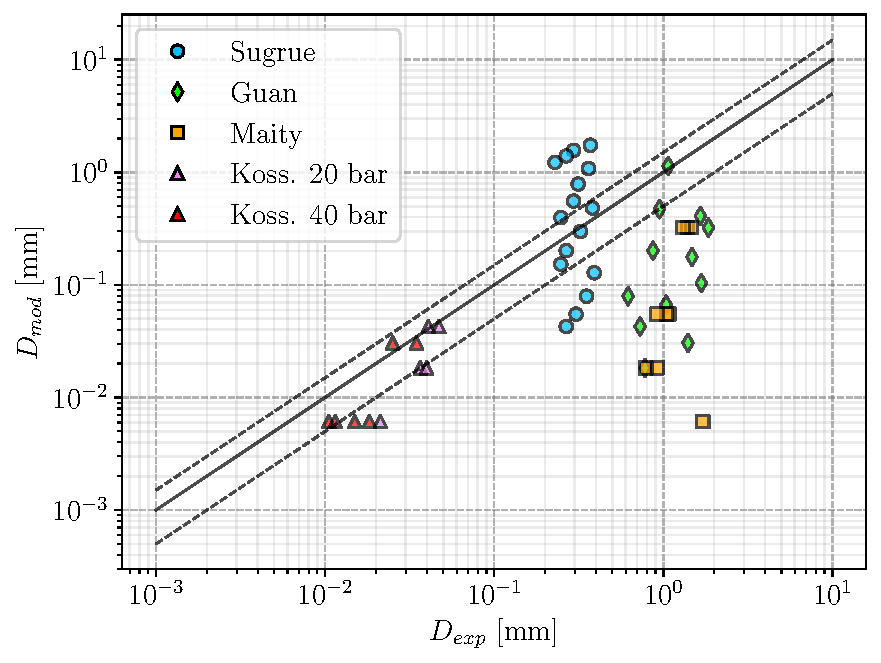
\includegraphics[width=0.5\linewidth]{img/forces/pred_nogrKoss4deg.pdf}
} 
\subfloat[Using Eq.\ref{eq:pred_gr}]{
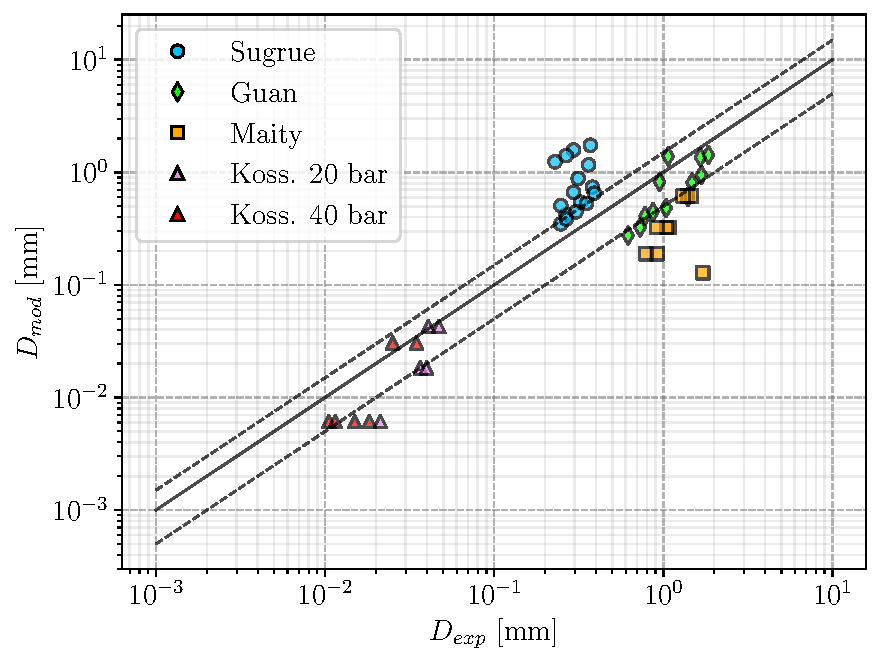
\includegraphics[width=0.5\linewidth]{img/forces/pred_grKoss4deg.pdf}
}
	\caption{$D_{d}$ predictions using $\dtheta = 4\degree$ for Kossolapov}	
	\label{fig:pred_Koss4deg}
\end{center}
\end{figure}




\begin{figure}[h!]
\begin{center}
\subfloat[$\Delta T_{w}=5.0$\degree C, $G_{L}=73.8~\debm$]{
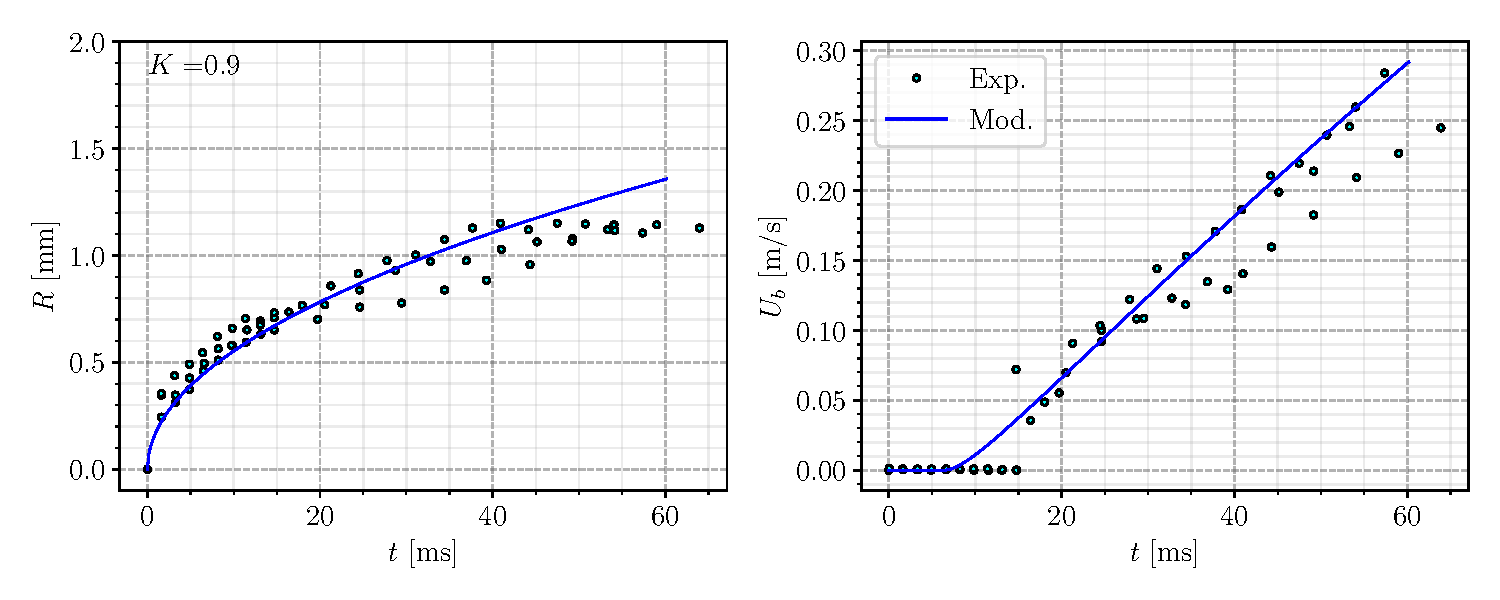
\includegraphics[width=0.9\linewidth]{img/forces/maity_V0p077.pdf}
} 
\\
\subfloat[$\Delta T_{w}=5.9$\degree C, $G_{L}=143.8~\debm$]{
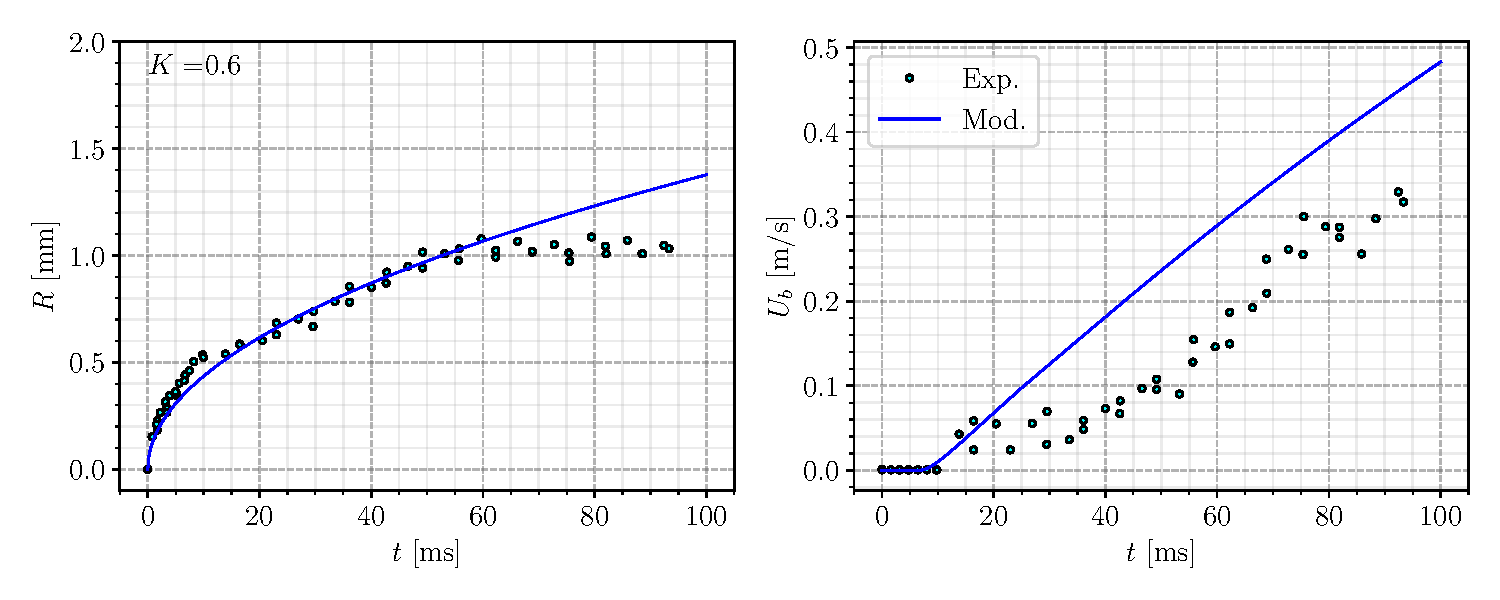
\includegraphics[width=0.9\linewidth]{img/forces/maity_V0p15.pdf}
}
\\
\subfloat[$\Delta T_{w}=5.9$\degree C, $G_{L}=239.6~\debm$]{
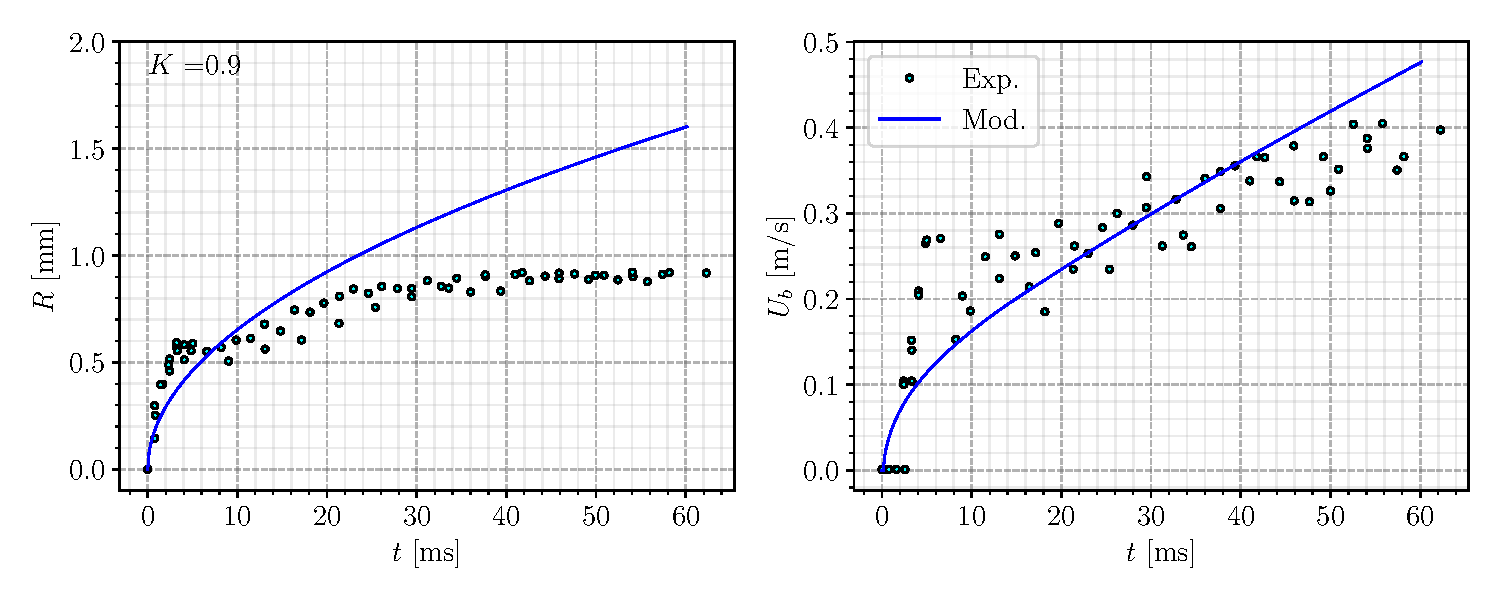
\includegraphics[width=0.9\linewidth]{img/forces/maity_V0p25.pdf}
}
	\caption{Bubble sliding velocity predictions on Maity cases}
	\label{fig:slide_maity}
\end{center}
\end{figure}



\begin{figure}[h!]
\begin{center}
\subfloat[$\phi_{w}=0.178$~MW/m\up{2}, $G_{L}=500~\debm$]{
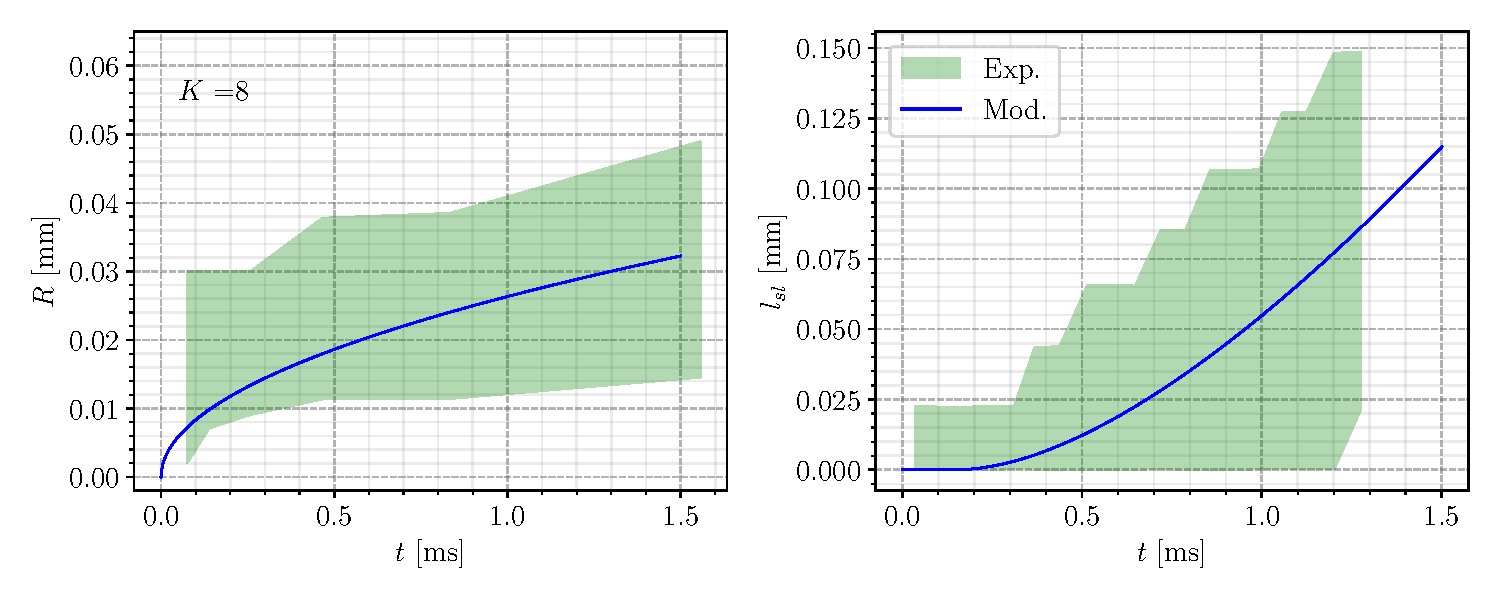
\includegraphics[width=0.9\linewidth]{img/forces/Koss_P20_G500.pdf}
} 
\\
\subfloat[$\phi_{w}=0.495$~MW/m\up{2}, $G_{L}=994~\debm$]{
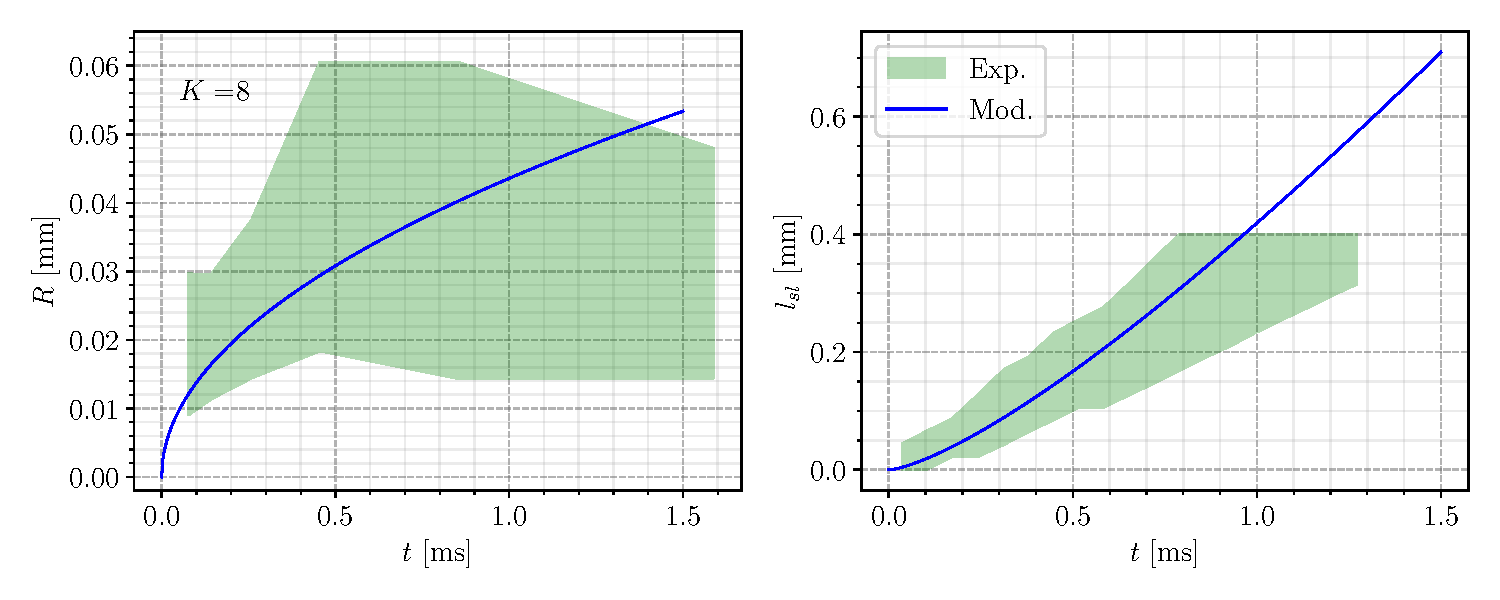
\includegraphics[width=0.9\linewidth]{img/forces/Koss_P20_G1000.pdf}
} 
\\
\subfloat[$\phi_{w}=0.487$~MW/m\up{2}, $G_{L}=1504~\debm$]{
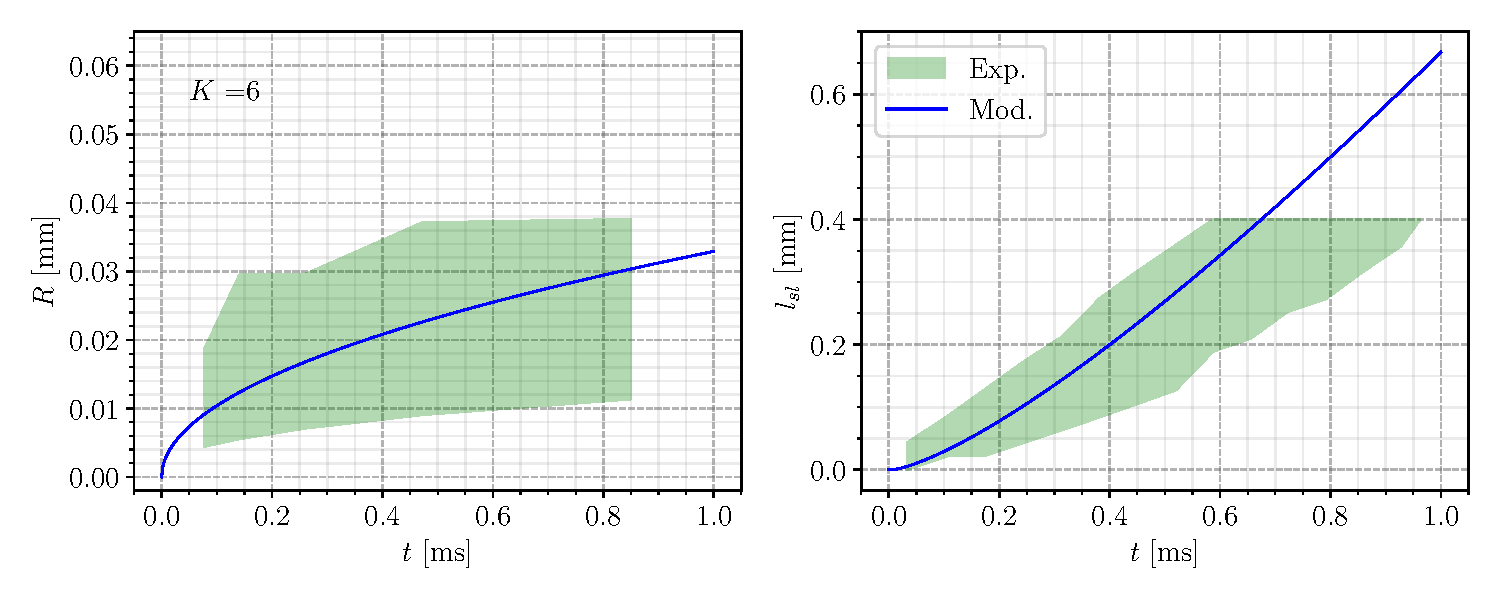
\includegraphics[width=0.9\linewidth]{img/forces/Koss_P20_G1500.pdf}
} 
	\caption{Bubble sliding length predictions on Kossolapov cases - $P=20$ bar}
	\label{fig:slide_koss_20bar}	
\end{center}
\end{figure}


\begin{figure}[h!]
\begin{center}
\subfloat[$\phi_{w}=0.291$~MW/m\up{2}, $G_{L}=500~\debm$]{
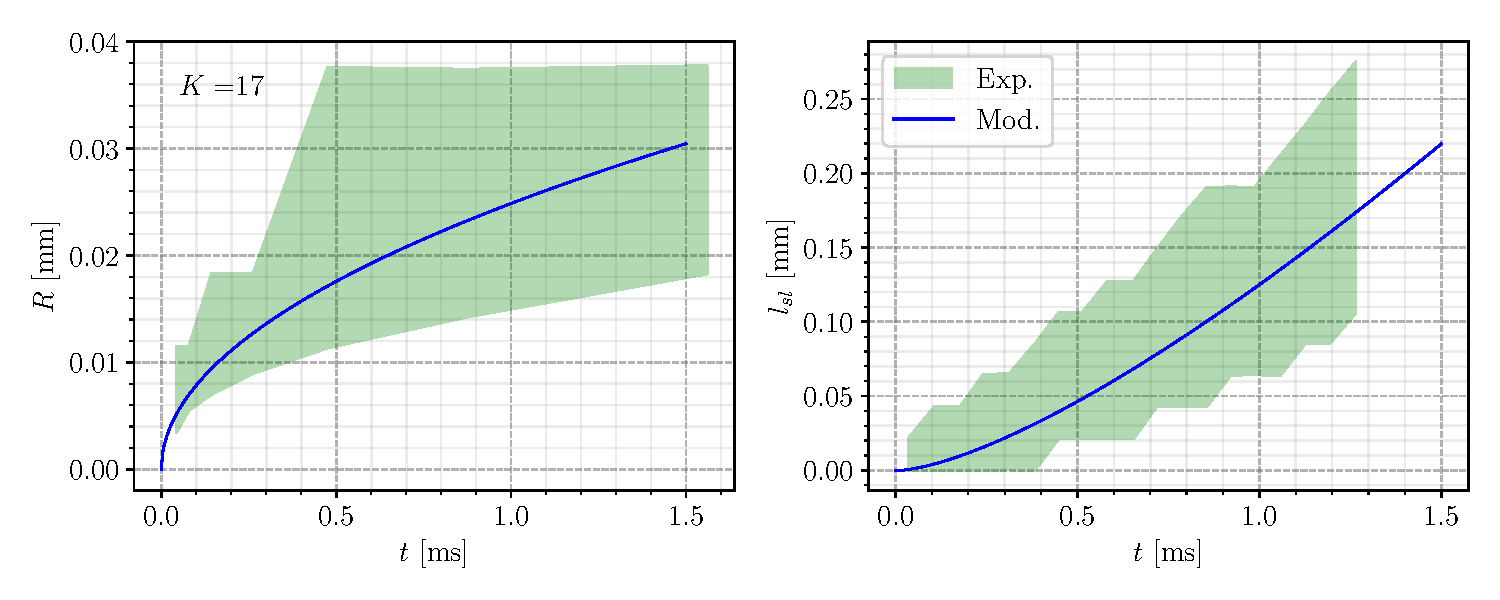
\includegraphics[width=0.9\linewidth]{img/forces/Koss_P40_G500.pdf}
} 
\\
\subfloat[$\phi_{w}=0.361$~MW/m\up{2}, $G_{L}=994~\debm$]{
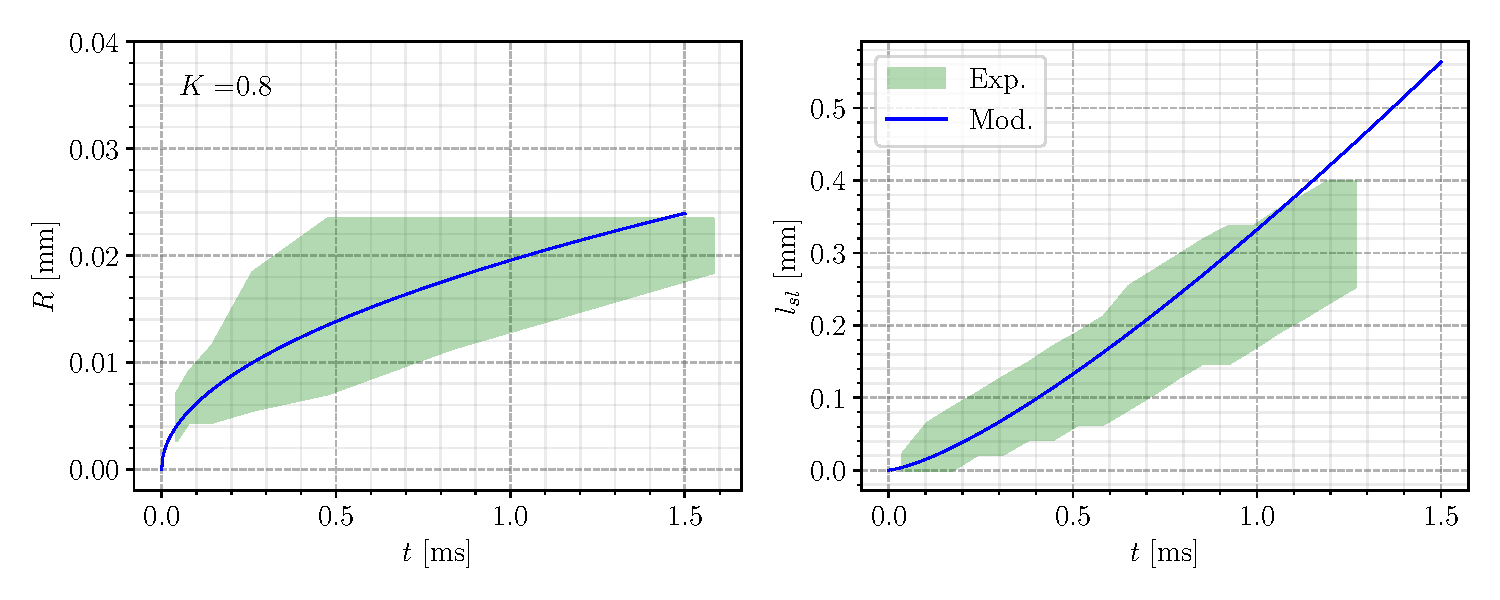
\includegraphics[width=0.9\linewidth]{img/forces/Koss_P40_G1000.pdf}
} 
\\
\subfloat[$\phi_{w}=0.613$~MW/m\up{2}, $G_{L}=1504~\debm$]{
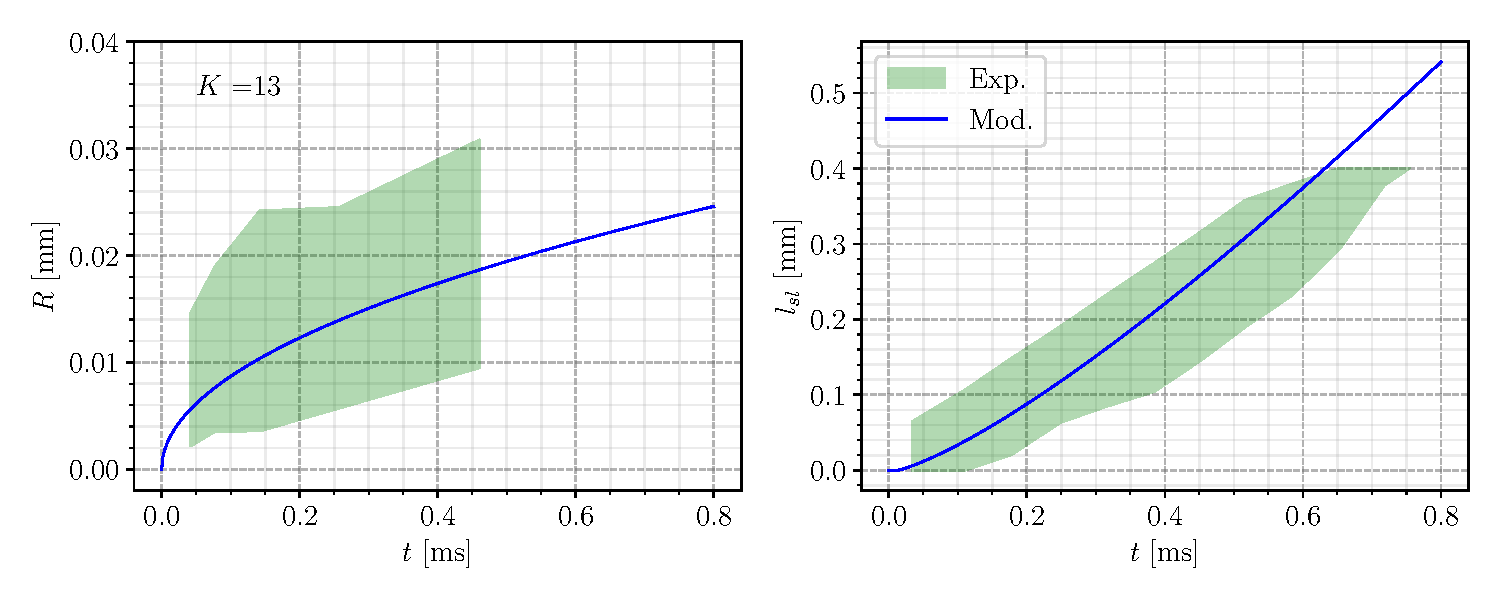
\includegraphics[width=0.9\linewidth]{img/forces/Koss_P40_G1500.pdf}
} 
	\caption{Bubble sliding length predictions on Kossolapov cases - $P=40$ bar}	
	\label{fig:slide_koss_40bar}
\end{center}
\end{figure}






\clearpage





\newpage

\newpage

When trying to understand the underlying physics behind departure and lift-off of growing bubbles on a wall, forces naturally come into the equations. Indeed, the critical diameters at which a bubble will leave its nucleation site to slide or lift-off from the surface are directly linked to the force balance applied to this very bubble.

\npar

Many authors have previsouly been tackling this issue to try to derive the whole force balance experienced by a bubble, starting with Klausner in 1993[CITE]. Since then, mechanistic approaches have been thoroughly studied to overcome empirical, correlation-based estimations of bubble departure and lift-off diameters[CITE]. The underlying idea is that if one manages to precisely compute the force balance applied to a bubble, it would lead to a high-fidelity representation of the bubble dynamics to evaluate its departure diameter $D_{d}$, sliding length $l_{sl}$, sliding velocity $U_{b}$ and lift-off diameter $D_{lo}$.  

\npar

However, the variety of hydrodynamics phenomena experienced by a boiling bubble in a flow makes the derivation of its force balance a very complicated task, in not impossible. This can only be achieved under many assumptions regardig bubble shape, external flow, etc. Moreover, the triggering of departure and lift-off can be associated to critical values of the force balance since many authors consider that the bubble starts moving when the balance is broken in one direction[CITE]. It is actually very delicate since it implies detecting a very small change in the whole force balance ($\sim \mathrm{nN}$) resulting from the sum of forces of much greater magnitude ($\sim \mu\mathrm{N}$)[CITE].

\npar

Nevertheless, studying the force balance can still provide interesting insights on bubble dynamics, particularly when comparing the impact of different forces depending on the operating conditions. That is why this chapter is dedicated to an analysis of the boiling bubble dynamics to try to understand a bit further the bubble behavior regarding the departure and sliding phenomenon in vertical flow boiling.



\begin{figure}[h!]
\centering

\fbox{


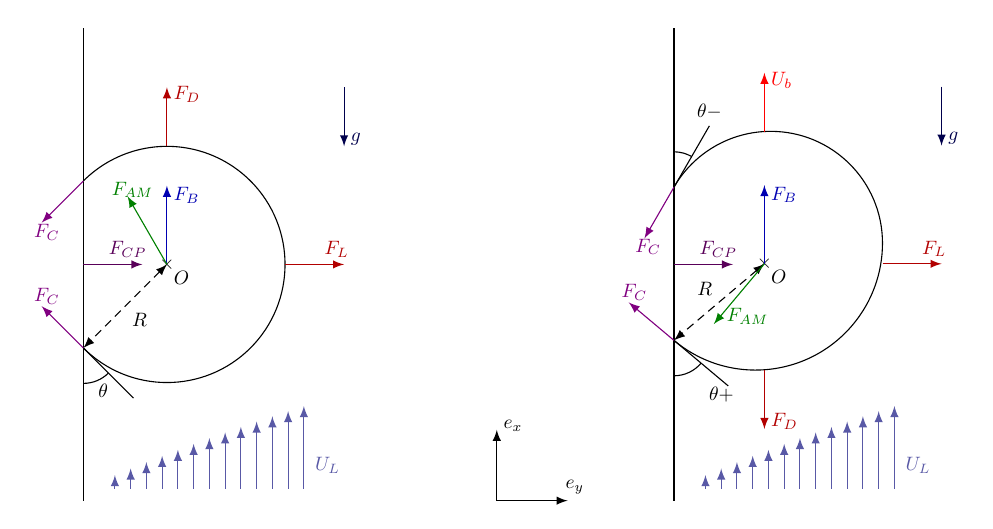
\begin{tikzpicture}[scale=3.0, every node/.style={scale=0.7}]


%%%Truncated sphere on a vertical wall

\coordinate (O1) at (0,0);
\coordinate (O2) at (0,2);

\draw (O1)--(O2);

\coordinate (Ob) at (0,1.0);

\tikzmath{\thet = 45; \thetrad= \thet * pi / 180; \ray=0.5; \rw=\ray * sin(\thetrad r);};


\coordinate (Oarc) at ($(Ob)-(0,{\ray * sin(\thetrad r)})$);
\draw (Oarc) arc({(-pi+\thetrad ) r}:{(pi-\thetrad ) r}:\ray);

%Upstream angle
\draw (Oarc) --++(-90+\thet:0.3);
\draw ($(Oarc)+(0,-0.15)$) arc(-90:-90+\thet:0.15) node[near end, below]{$\theta$};

%%Downstream angle
%\coordinate (Oarc2) at ($(Oarc) - (2*\rw,0)$);
%\draw (Oarc2) --++(180-\thet:0.3);
%\draw ($(Oarc2)+(-0.15,0)$) arc(180:180-\thet:0.15) node[near end, left]{$\alpha$};

%Center and radius

\coordinate (Cb) at ($(Ob)+({\ray*cos(\thetrad r)},0 )$);
\draw (Cb) node{$\times$} node[below right]{$O$};

\draw[densely dashed, <->, >=latex] (Cb) -- (Oarc) node[midway, below right]{$R$};


%%Forces

\draw[->, >=latex, violet!70!black] (Ob)--++(\ray/2,0) node[near end, above]{$\vect{F_{CP}}$};

\draw[->, >=latex, red!70!black!] ($(Cb)+(\ray,0)$)--++(\ray/2,0) node[very near end, above]{$\vect{F_{L}}$};
\draw[->, >=latex, red!70!black!] ($(Cb)+(0,\ray)$)--++(0,\ray/2) node[very near end, right]{$\vect{F_{D}}$};

\coordinate (Oarc2) at ($(Oarc)+(0,{2*\rw})$);
\draw[->, >=latex, violet] (Oarc)--++(90+\thet:\ray/2) node[very near end, above]{$\vect{F_{C}}$};
\draw[->, >=latex, violet] (Oarc2)--++(-90-\thet:\ray/2) node[very near end, below]{$\vect{F_{C}}$};

\draw[->, >=latex, blue!70!black] (Cb)--++(0,\ray/1.5) node[very near end, right]{$\vect{F_{B}}$};


\draw[->, >=latex, green!50!black!] (Cb)--++(90+\thet/1.5:\ray/1.5) node[very near end, above]{$\vect{F_{AM}}$};

%Gravity

\draw[->, >=latex, blue!30!black]  ($(Cb)+({1.5*\ray},{1.5*\ray})$)--++(0,-\ray/2) node[very near end, right]{$\vect{g}$};


%Flow arrows
\foreach \i in {2,...,14} 
{
\coordinate (Oloc) at ($(O1)+(\i/15,0.05)$);
\draw[->,>=latex, gray!70!blue] (Oloc)--++(0,{ln(1+0.03*\i)});
}
\draw[gray!70!blue] ($(Oloc)+(0.1,0.1)$) node{$\vect{U_{L}}$};

%Referential vectors
\coordinate (Ovect) at (1.75,0);
\draw[->, >=latex] (Ovect)--++(0.3,0) node[very near end, above right]{$\vect{e_{y}}$};
\draw[->, >=latex] (Ovect)--++(0,0.3) node[very near end, above right]{$\vect{e_{x}}$};




%Tilted bubble
\coordinate (Ob2) at (2.5,1.0);

\coordinate (O1) at (2.5,0);
\coordinate (O2) at (2.5,2);
\draw (O1)--(O2);

\tikzmath{\thet = 40; \thetrad= \thet * pi / 180;
\dthet=10; \dthetrad=\dthet*pi/180;
\thetadvrad=\thetrad - \dthetrad;
\thetrecrad=\thetrad + \dthetrad;
\thetadv=\thetadvrad*180/pi;
\thetrec=\thetrecrad*180/pi;
\ray=0.5; 
\rayadv=\ray *(1+cos(\thetrad r))/(1+ cos(\thetadvrad r);
\rayrec=\ray *(1+cos(\thetrad r))/(1+ cos(\thetrecrad r);};

\coordinate (Oarc) at ($(Ob2)-(0,{\ray * sin(\thetrad r)})$);


\draw (Oarc) arc({-pi+(\thetrecrad)) r}:{0 r}:\rayrec) arc ({0 r}:{pi-(\thetadvrad)) r}:\rayadv);

%Upstream angle
\draw (Oarc) --++(-90+\thetrecrad r:0.3) node[very near end, below]{$\theta + \dtheta$};
\draw ($(Oarc)+(0,-0.15)$) arc(-90:-90+\thetrecrad r:0.15) ;

%Downstream angle
\coordinate (Oarc2) at ($(Oarc) + (0,{\rayadv * sin(\thetadvrad r) + \rayrec * sin(\thetrecrad r)})$);
\draw (Oarc2) --++({90-(\thetadvrad r)}:0.3);
\coordinate (angadv) at ($(Oarc2) +({90-(\thetadvrad r)}:0.3)$);
\draw (angadv)  node[above]{$\theta - \dtheta $};
\draw ($(Oarc2)+(0,+0.15)$) arc(90:{90-(\thetadvrad r)}:0.15);



%Center and radius

\coordinate (Cb) at ($(Oarc2)+( {\ray * cos(\thetrad r)} , {-0.5 * (\rayadv * sin(\thetadvrad r) + \rayrec  * sin(\thetrecrad r) )})$);
\draw (Cb) node{$\times$} node[below right]{$O$};

\draw[densely dashed, <->, >=latex] (Cb) -- (Oarc) node[midway, above left]{$R$};


%Inclination angle

%\draw[densely dotted] (Cb) --++ (0.7,0);
%\draw[densely dotted] (Cb) --++ ({(1*\dthetrad r)}: 0.7 );
%\draw ($(Cb) + (0.3,0)$) arc(0: {(\dthetrad r)}:0.3)  node[midway, right]{$\dtheta$};
%
%



%%Forces

\draw[->, >=latex, violet!70!black] (Ob2)--++(\ray/2,0) node[near end, above]{$\vect{F_{CP}}$};

\draw[->, >=latex, red!70!black!] ($(Cb)+(\ray,0)$)--++(\ray/2,0) node[very near end, above]{$\vect{F_{L}}$};
\draw[->, >=latex, red!70!black!] ($(Cb)+(0,-\rayadv*0.95)$)--++(0,-\ray/2) node[very near end, right]{$\vect{F_{D}}$};
\draw[->, >=latex, red] ($(Cb)+(0,+\rayrec*1.04)$)--++(0,+\ray/2) node[very near end, right]{$\vect{U_{b}}$};


\draw[->, >=latex, violet] (Oarc)--++(90+\thetrec:\ray/2) node[very near end, above]{$\vect{F_{C}}$};
\draw[->, >=latex, violet] (Oarc2)--++(-90-\thetadv:\ray/2) node[very near end, below]{$\vect{F_{C}}$};

\draw[->, >=latex, blue!70!black] (Cb)--++(0,\ray/1.5) node[very near end, right]{$\vect{F_{B}}$};


\draw[->, >=latex, green!50!black!] (Cb)--++(90-\thet:-\ray/1.5) node[very near end, right]{$\vect{F_{AM}}$};

%Gravity

\draw[->, >=latex, blue!30!black]  ($(Cb)+({1.5*\ray},{1.5*\ray})$)--++(0,-\ray/2) node[very near end, right]{$\vect{g}$};



%Flow arrows
\foreach \i in {2,...,14} 
{
\coordinate (Oloc) at ($(O1)+(\i/15,0.05)$);
\draw[->,>=latex, gray!70!blue] (Oloc)--++(0,{ln(1+0.03*\i)});
}
\draw[gray!70!blue] ($(Oloc)+(0.1,0.1)$) node{$\vect{U_{L}}$};



\end{tikzpicture}

}

\caption{Bubble force balance in vertical flow boiling}
\end{figure}


\section{Establishment of the force balance for a bubble on a vertical wall }


In this section, we wish to detail expressions of the different forces experienced by the bubble and to compare their magnitude in order to assess which will be predominant in the departure and lift-off process.

\subsection{Bubble shape : Geometrical definitions}

\label{subsec:geom_bub}

In order to clearly express each of the considered forces, assumptions regarding the shape of the bubble nucleating at the wall are needed.

\npar

Here, we assume that the bubbles will mostly have the shape of a truncated sphere with respect to the contact angle $\theta_{s}$ (Fig. \ref{fig:bub_shape}), being a thermophysical property of the fluid and the  wall. This assumption can thoroughly be discussed since many experimental measurements and visualizations have shown that in the case of low pressure boiling, bubbles tend te be strongly deformed depending on the flow conditions (\textsc{Maity}, \textsc{Estrada-Pérez} \etal, etc.) thus casting doubts on spherical or quasi-spherical hypotheses.

\npar
On the other hand, experiments conducted by \textsc{Kossolapov} found that in vertical flow boiling, increasing pressure leads to smaller and less deformable bubbles. Thus, supposing a truncated spherical shape could be relevant to model nucleating bubbles on a heater surface. Moreover, working on highly deformed bubbles would undoubtedly imply complicated calculations and extra parameters to account for.

\textsc{Kossolapov}'s measurements also concluded that bubbles' inclination due to the flow nearly disappears at high pressures. However, since bubble tilt plays a great role in the surface tension force, we consider an angle tilt $\dtheta$ compared to the static contact angle $\theta_{s}$.

\begin{figure}[h!]
\centering
\fbox{

\renewcommand{\dalpha}{\text{d}\alpha}

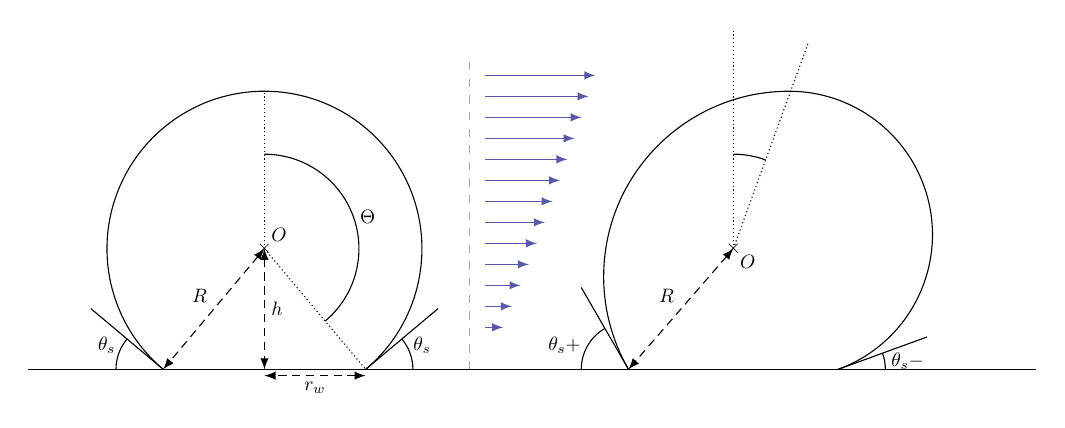
\begin{tikzpicture}[scale=4.0, every node/.style={scale=0.7}]


\coordinate (O) at (0,0);
\coordinate (A2) at (1.4,0);
\coordinate (A) at (3.2,0);


%Sections and wall
\draw (O) -- (A);
%\draw ($(O)-(0,0.05)$) -- ($(A)-(0,0.05)$);
%\foreach \i in {0,...,15}
%{
%\draw (\i*0.2,0) -- (\i*0.2+0.1,-0.05);
%}

\draw[dashed, gray!70!white] (A2) --++ (0,1);


%Non-tilded bubble
\coordinate (Ob) at (0.75,0);

\tikzmath{\alph = 40; \alphrad= \alph * pi / 180; \ray=0.5; \rw=\ray * sin(\alphrad r); \h=\ray * cos(\alphrad r);};


\coordinate (Oarc) at ($(Ob)+({\ray * sin(\alphrad r)},0)$);
\draw (Oarc) arc({-(pi/2-\alphrad) r}:{(pi+pi/2-\alphrad) r}:\ray);

%Right angle
\draw (Oarc) --++(\alph:0.3);
\draw ($(Oarc)+(0.15,0)$) arc(0:\alph:0.15) node[near end, right]{$\theta_{s}$};

%Left angle
\coordinate (Oarc2) at ($(Oarc) - (2*\rw,0)$);
\draw (Oarc2) --++(180-\alph:0.3);
\draw ($(Oarc2)+(-0.15,0)$) arc(180:180-\alph:0.15) node[near end, left]{$\theta_{s}$};

%Center and radius

\coordinate (Cb) at ($(Ob)+(0,{\ray*cos(\alphrad r)} )$);
\draw (Cb) node{$\times$} node[above right]{$O$};

\draw[densely dashed, <->, >=latex] (Cb) -- (Oarc2) node[midway, above left]{$R$};


%Angular portion

\draw[densely dotted] (Cb)--++(0,\ray);
\draw[densely dotted] (Cb) -- (Oarc);

\draw ($(Cb)+(0,0.3)$) arc(90:-(90-\alph):0.3) node[midway, right]{$\Theta$};

%Bubble foot
\draw[<->,>=latex, densely dashed] ($(Oarc)-(0,0.02)$) --++ (-\rw,0) node[midway,below]{$r_{w}$};
%Bubble height
\draw[<->, >=latex, densely dashed] (Cb)--++(0,-\h) node[midway, right]{$h$};


%Tilted bubble
\coordinate (Ob2) at (2.25,0);

\tikzmath{\alph = 40; \alphrad= \alph * pi / 180;
\dalph=20; \dalphrad=\dalph*pi/180;
\alphadvrad=\alphrad - \dalphrad;
\alphrecrad=\alphrad + \dalphrad;
\ray=0.5; 
\rayadv=\ray *(1+cos(\alphrad r))/(1+ cos(\alphadvrad r);
\rayrec=\ray *(1+cos(\alphrad r))/(1+ cos(\alphrecrad r);};

\coordinate (Oarc) at ($(Ob2)+({\ray * sin(\alphrad r)},0)$);


\draw (Oarc) arc({-(pi/2-(\alphadvrad)) r}:{(pi/2) r}:\rayadv) arc ({(pi/2) r}:{(pi+pi/2-(\alphrecrad)) r}:\rayrec);

%Right angle
\draw (Oarc) --++(\alphadvrad r:0.3);
\draw ($(Oarc)+(0.15,0)$) arc(0:\alphadvrad r:0.15) node[midway, right]{$\theta_{s} - \dtheta$};

%Left angle
\coordinate (Oarc2) at ($(Oarc) - ({\rayadv * sin(\alphadvrad r) + \rayrec * sin(\alphrecrad r)},0)$);
\draw (Oarc2) --++({180-(\alphrecrad r)}:0.3);
\draw ($(Oarc2)+(-0.15,0)$) arc(180:{180-(\alphrecrad r)}:0.15) node[midway, left]{$\theta_{s} + \dtheta $};



%Center and radius

\coordinate (Cb) at ($(Oarc)+( -{0.5 * (\rayadv * sin(\alphadvrad r) + \rayrec  * sin(\alphrecrad r) } , {\ray * cos(\alphrad r)} )$);
\draw (Cb) node{$\times$} node[below right]{$O$};

\draw[densely dashed, <->, >=latex] (Cb) -- (Oarc2) node[midway, above left]{$R$};


%Inclination angle

\draw[densely dotted] (Cb) --++ (0,0.7);
\draw[densely dotted] (Cb) --++ ({90 - (1*\dalphrad r)}: 0.7 );
\draw ($(Cb) + (0,0.3)$) arc(90: {90 - (\dalphrad r)}:0.3)  node[midway, above]{$\dtheta$};



%Flow arrows
\foreach \i in {2,...,14} 
{
\coordinate (Oloc) at ($(A2)+(0.05,\i/15)$);
\draw[->,>=latex, gray!70!blue] (Oloc)--++({ln(1+0.03*\i)},0);
}



\end{tikzpicture}

}
\caption{Sketch of the supposed bubble shape with (right) and without inclination (left).}
\label{fig:bub_shape}

\end{figure}



The resulting bubble's volume $V_{b}$ and projected area in the direction of the flow $S_{p}$ can then be computed using the spherical coordinates system and defining the total angular portion covered by the bubble as $\Theta = \pi - \theta_{s}$, the bubble foot radius $r_{w}=R \sin{\theta_{s}}$ and the distance between the center of the bubble and the surface $h=R\parth{1+\cos{\theta_{s}}}$, we have :

\begin{align}
V_{b} &= \underbrace{ \int_{r=0}^{R} \int_{\theta=0}^{\Theta} \int_{\varphi=0}^{2\pi} r^{2}\sin{\theta} \text{d}r ~\text{d}\theta~ \text{d}\varphi }_{\text{Spherical volume}}+ \underbrace {\frac{1}{3}\pi r_{w}^{2}h}_{\text{Conic volume}}
=\frac{4}{3}\pi R^{3} \crocht{ \frac{1}{4} \parth{2-\cos{\theta_{s}}}\parth{1+\cos{\theta_{s}}}^{2} } \\
S_{p}&= \underbrace{\int_{r=0}^{R}\int_{\theta=-\Theta}^{\Theta}r \text{d}r ~ \text{d}\theta}_{\text{Circular area}} + \underbrace{r_{w}h}_{\text{Triangular area}} = \pi R^{2} \crocht{1-\frac{\theta_{s}}{\pi} + \frac{\sin{2\theta_{s}}}{2\pi} } 
\end{align}


Thus, we can define shape factors that represent the ratio between the volume and projected areas of the truncated sphere compared to a complete sphere : 

\begin{align}
f_{V}\left(\theta_{s}\right)=\frac{V_{ts}}{V_{s}}=\frac{1}{4}\left(2-\cos{\theta_{s}}\right)\left(1+\cos{\theta_{s}}\right)^{2}\\
f_{S_{p}}\left(\theta_{s}\right)=\frac{S_{p,ts}}{S_{p,s}}=1-\frac{\theta_{s}}{\pi}+\frac{\sin{2\theta_{s}}}{2\pi}
\end{align}

Subscripts $s$ and $ts$ respectively denoting spherical and truncated spherical shapes.


\npar

Using those assomptions, we can thus express the volume of vapor generated for a single bubble up to its lift-off diameter $D_{lo}=2R_{lo}$ (Eq. \ref{eq:boil_vol}) :

\begin{align}
\label{eq:boil_vol}
V_{b}=\frac{4}{3}\pi \bluemath{R_{lo}}^{3} f_{V}\parth{\theta_{s}} = \frac{\pi \bluemath{D_{lo}}^{3}}{6} f_{V}\parth{\theta_{s}}
\end{align}

As described in Section \ref{subsec:geom_bub}, we consider a bubble with a potential inclination $\dalpha$ from the static contact angle $\theta_{s}$. Thus, the downstream contact angle is $\theta_{d}=\theta_{s} - \dtheta$ and the upstream contact angle is $\theta_{u}=\theta_{s} + \dtheta$ (Figure \ref{fig:bub_shape}).

\npar

To estimate the bubble foot radius $r_{w}$ of such a bubble, we can express it as the average between the two foot diameters for the advancing and receding contact angles :

\begin{align}
r_{w} &= \frac{1}{2}\parth{\sin{\theta_{d}}R + \sin{\theta_{u}}R} = R~\sin{\theta_{s}}\cos{\dtheta}
\end{align}

\npar

In the following subsections, the vectors $\vect{e_{\|}}$ and $\vect{e_{\bot}}$ respectively represent the colinear and orthogonal vector to the wall surface.


\begin{figure}[h!]


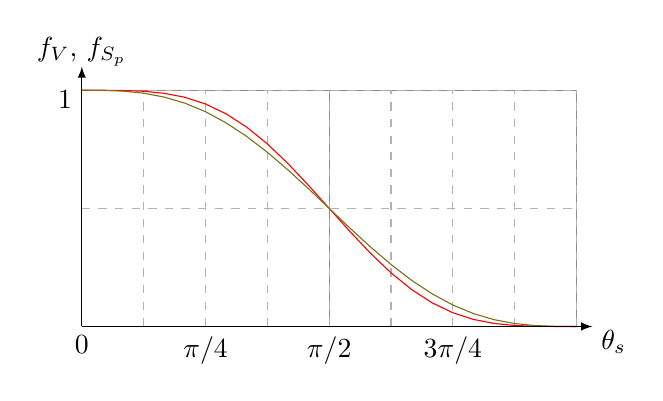
\begin{tikzpicture}[yscale=3, xscale=2]

\tikzmath{\alph1=70;}
\draw[gray!90!] (0,0) grid[ystep=1,xstep=pi/2](pi,1);
\draw[gray!60!, dashed] (0,0) grid[ystep=0.5, xstep=pi/8](pi,1);
%\draw[gray!60!, densely dotted] (0,0) grid[step=pi/4](4,1);


%\draw [domain=-pi:pi] plot (\x,{sin(\x r)});
%\draw[domain=0:pi] plot(\x, {cos(\x r)});
\draw [domain=0:pi, red] plot(\x,{0.25*(2-cos(\x r))*((1+cos(\x r))^2)}); %f_V
\draw [domain=0:pi, olive!80!black] plot(\x,{1-\x/pi + sin((2*\x) r)/(2*pi)}); %f_Sp
%\draw [domain=0:pi, blue] plot(\x,{(1-cos(\x r)^2)}); %f_G

\draw[->,>=latex,black] (0,0)--(0,1.1) node[very near end, above=0.3cm]{$\redmath{f_{V}}$, $\greenmath{f_{S_{p}}}$} node[very near start, below=0.4cm]{$0$} node[very near end, left]{$1$};
\draw[->,>=latex,black] (0,0)--(pi+0.1,0) node[very near end, below=0.2cm, right=0.8cm]{$\theta_{s}$};

\draw (pi/4,0) node[below]{$\pi/4$};
\draw (pi/2,0) node[below]{$\pi/2$};
\draw (3*pi/4,0) node[below]{$3\pi/4$};


\end{tikzpicture}
\hfill
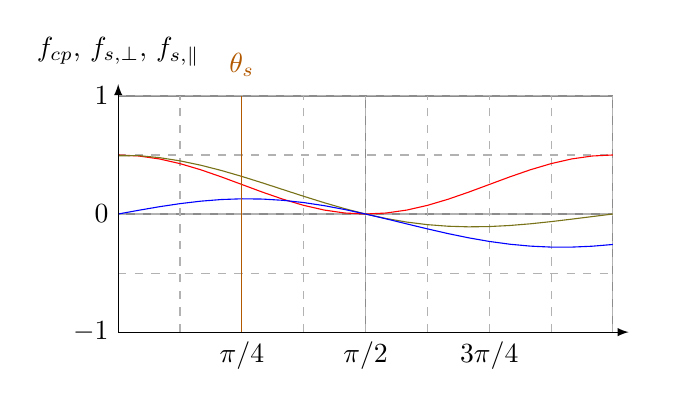
\begin{tikzpicture}[xscale=2, yscale=1.5]

\tikzmath{\alphdeg=45; \alphrad=\alphdeg*pi/180;}
\draw[gray!90!] (0,-1) grid[xstep=pi/2,ystep=1](pi,1);
\draw[gray!60!, dashed] (0,-1) grid[xstep=pi/8,ystep=0.5](pi,1);

%\draw [domain=-pi:pi] plot (\x,{sin(\x r)});
%\draw[domain=0:pi] plot(\x, {cos(\x r)});
\draw [domain=0:pi, red] plot(\x,{(sin(\alphrad r)^2)*(cos(\x r)^2)}); %f_cp
\draw [domain=0.001:pi, olive!80!black] plot(\x,{(sin(\alphrad r)^2)*sin(2*\x r)/(2*\x)}); %f_s,orth
\draw [domain=0:pi, blue] plot(\x,{1.215*\x*(sin(\alphrad r)^2)*(cos(\x r)^2)/((pi/2)^2 - \x^2)}); %f_s,parl


\draw[->,>=latex,black] (0,-1)--(0,1.1) node[very near end, above=0.5cm]{$\redmath{f_{cp}}$, $\greenmath{f_{s,\bot}}$, $\bluemath{f_{s,\|}}$};
\draw (0,0) node[left]{$0$};
\draw (0,1) node[left]{$1$};
\draw (0,-1) node[left]{$-1$};
\draw[->,>=latex,black] (0,-1)--(pi+0.1,-1) node[very near end, below=0.2cm, right=0.8cm]{$\dtheta$};

\draw (pi/4,-1) node[below]{$\pi/4$};
\draw (pi/2,-1) node[below]{$\pi/2$};
\draw (3*pi/4,-1) node[below]{$3\pi/4$};

\draw[orange!70!black] (\alphrad, -1) -- (\alphrad,1) node[very near end, above=0.5cm]{$\theta_{s}$};

\end{tikzpicture}
\caption{Representation of the shape functions}
\end{figure}


\subsection{Buoyancy force}

The well-known buoyancy force, also called Archimedes force, is computed by integration of the hydrostatic pressure exterted by the liquid over the bubble's surface and results in the difference between the gravity forces experienced by the vapour bubble and the equivalent liquid volume. The expression of this force $\vect{F_{B}}$ is aligned with the gravity vector $\vect{g}=-g\vect{e_{x}}$.

\begin{align}
\vect{F_{B}}&=V_{b}\parth{\rho_{V}-\rho_{L}}\vect{g}=\frac{4}{3}\pi R^{3}f_{V}\parth{\theta_{s}}\parth{\rho_{L}-\rho_{V}}g\vect{e_{x}}
\end{align}

\subsection{Contact Pressure force}

The contact pressure force arises due to the pressure difference between the center of the bubble and the surrounding liquid. This pressure jump can be computed using \textsc{Laplace}'s expression $\Delta P = 2\sigma / R_{c}$ where $R_{c}$ is the curvature radius of the bubble's interface, being equal to $R$ in the case of a spherical bubble. This pressure difference is then applied over the bubble foot area and results in a repelling force from the bubble's point of view, giving the resulting expression of $\vect{F_{CP}}$.

\begin{align}
\vect{F_{CP}}&=\frac{2\sigma}{R_{c}}\frac{\pi d_{w}^{2}}{4}\vect{e_{y}} \approx 2\sigma \pi R \underbrace{\sinsq{\theta} \cossq{\dtheta}}_{f_{CP}}\vect{e_{\bot}} =2\pi R \sigma f_{CP}\parth{\theta, \dtheta}\vect{e_{x}}\\
\end{align}

\subsection{Capillary force}

The capillary or surface tension force results from the integration of the effort exerted over the triple contact line between the vapor inside the bubble, the surrounding liquid and the wall. This force has been derived by \textsc{Klausner}[CITE] for a inclined bubble, yielding for each direction regarding the wall :

\begin{align}
\vect{F_{C}}&=-1.25 d_{w}\sigma \frac{\pi\parth{\theta_{u}-\theta_{d}}}{\pi^{2}-\parth{\theta_{u}-\theta_{d}}^{2}}\parth{\sin{\theta_{u}}+\sin{\theta_{d}} }\vect{e_{x}} -d_{w} \sigma \frac{\pi}{\theta_{u}-\theta_{d}}\parth{\cos{\alpha_{d}}- \cos{\alpha_{u}}}\vect{e_{y}} \\
%
&\approx -\pi R \sigma \underbrace{\crocht{1.25\ \frac{2\dtheta}{\parth{\frac{\pi}{2}}^{2}-\dtheta^{2}}\sin{\theta_{s}}^{2}\cos{\dtheta}^{2}}}_{f_{C,x}} \vect{e_{x}} - \pi R \sigma \underbrace{\crocht{2\ \sin{\theta_{s}}^{2}\frac{\sin{2\dtheta}}{2\dtheta}}}_{f_{C,y}}\vect{e_{y}}\\
%
&= -\pi R \sigma f_{C,x}\parth{\theta_{s}, \dtheta}\vect{e_{x}} - \pi R \sigma f_{C,y}\parth{\theta_{s}, \dtheta} \vect{e_{y}}
\end{align}

\npar

\subsection{Added Mass force of a growing bubble}

Added mass effects are experienced by the bubble :

\begin{itemize}
\item when its boundary is moving during its growth
\item when accelerating while sliding on the wall 
\item when the surrounding liquid is accelerating
\end{itemize}

We consider a spherical cap shaped bubble standing on a plane wall and facing an uniform liquid velocity $U$. In this situation, Van Der Geld derived the potential flow around the bubble and expressed the liquid kinetic energy, obtaining : 

\begin{align}
T_{L}=\rho_{L}V_{b}\parth{ \frac{1}{2}\alpha \dot{y}^{2} + \frac{1}{2} \trb\dot{R}^{2}+\frac{1}{2}\psi \dot{R}\dot{y} + \frac{1}{2} \alpha_{2} U^{2} }
\end{align}
where $\alpha$, $\mathrm{tr}\parth{\beta}$, $\psi$ and $\alpha_{2}$ are polynomimals of $\lambda = \frac{R}{2h}$. We also have $x$ and $y=h$ denoting the coordinates of the geometrical center of the bubble.

Therefore, we can write those coefficients in the following form : 

\begin{align}
\alpha = \sum_{k=0}^{n}\alpha_{k}\frac{R^{k}}{2^{k}y^{k}}
\end{align}

If we suppose that the generalized coordinates and velocities $x$, $\dot{x}$, $y$, $\dot{y}$, $R$, and $\dot{R}$, we can use the expression of the kinetic energy of the fluid to apply Lagrange's equations to derive the added mass forces on the bubble in both direction parallel and normal to the wall :

\begin{align}
F_{AM,x}&=-\dpartial{}{t}\parth{\dpartial{T_{L}}{\dot{x}}}+\dpartial{T_{L}}{x}\\
F_{AM,y}&=-\dpartial{}{t}\parth{\dpartial{T_{L}}{\dot{y}}}+\dpartial{T_{L}}{y}
\end{align}

In the case of the sliding bubble, we replace the uniform liquid velocity $U$ by the relative velocity experienced by the bubble $U_{rel}=U_{liq}-\dot{x}$ where $U_{liq}$ is the uniform surrounding liquid velocity and $\dot{x}$ the velocity of the center of the bubble, which is the sliding velocity of the bubble. Yielding :



\begin{align}
T_{L}=\frac{\rho_{L}V_{b}}{2}\parth{\alpha \dot{y}^{2} +\mathrm{tr}\parth{\beta}\dot{R}^{2}+\psi \dot{R}\dot{y} +\alpha_{2} \parth{U_{liq}-\dot{x}}^{2} }
\end{align}
 

\paragraph{Added mass in $x$ direction}

Parallel to the wall, since $\lambda$ depends on $y$ and $R$, it is independent of $\dot{x}$, yielding zero-derivatives for the added mass coefficients. We can write :

\begin{align}
\dpartial{T_{L}}{\dot{x}}&=\frac{\rho_{L}V_{b}}{2}\alpha_{2} \dpartial{\parth{ \parth{U_{liq}-\dot{x}}^{2}} }{\dot{x}}\\
&= \rho_{L}V_{b}\alpha_{2}\parth{\dot{x}-U_{liq}}\\
\end{align}\\

As for the time derivatives, we have : 

\begin{align}
\dpartial{V_{b}}{t}&=\dpartial{\frac{4}{3}\pi R^{3}}{t} = 4\pi R^{2} \dot{R}\\
\dpartial{\lambda}{t}&=\frac{\dot{R}~2y-R~2\dot{y}}{4y^{2}}=\lambda\parth{ \frac{\dot{R}}{R} - \frac{\dot{y}}{y}  }=\lambda \parth{\frac{\dot{R}}{R}-2\lambda \frac{\dot{y}}{R}}=\frac{\lambda}{R}\parth{\dot{R}-2\lambda \dot{y}}\\
\dpartial{\alpha}{t}&=\sum_{k=0}^{n}\alpha_{k}\dpartial{\lambda ^{k}}{t} = \sum_{k=0}^{n}\alpha_{k}~k\lambda ^{k-1} \dpartial{\lambda}{t} = \parth{ \frac{\dot{R}}{R} - \frac{\dot{y}}{y}  }\underbrace{ \sum_{k=0}^{n}\alpha_{k}~k\lambda^{k} }_{\tilde{\alpha}} = \frac{1}{R}\parth{\dot{R}-2\lambda \dot{y}}\tilde{\alpha}
\end{align}

Yielding : 

\begin{align}
\dpartial{}{t}\parth{ \dpartial{T_{L}}{\dot{x}}}&=\rho_{L}\crocht{ 4\pi R^{2} \dot{R} \alpha_{2}\parth{\dot{x}-U_{liq}}+\frac{4}{3}\pi R^{3}\parth{ \frac{\dot{R}}{R} - \frac{\dot{y}}{y} }\tilde{\alpha_{2}}\parth{\dot{x}-U_{liq}}+\frac{4}{3}\pi R^{3}\alpha_{2} \ddot{x} } \\
&=4\pi R^{2} \rho_{L}\crocht{ \alpha_{2}\dot{R}\parth{\dot{x}-U_{liq}}+\frac{\tilde{\alpha_{2}}}{3}\parth{\dot{R}- 2\lambda \dot{y} }\parth{\dot{x}-U_{liq}} + \frac{R}{3}\alpha_{2}\ddot{x} }\\
&=4 \pi R^{2} \rho_{L}\crocht{\parth{\alpha_{2}+\frac{\tilde{\alpha_{2}}}{3}}\dot{R}\parth{\dot{x}-U_{liq}}-\frac{2}{3}\lambda \tilde{\alpha_{2}}\dot{y}\parth{\dot{x}-U_{liq}}+\frac{R}{3}\alpha_{2}\ddot{x} }
\end{align}

We also have, with the independence of the variables :

\begin{align}
\dpartial{T_{L}}{x}&=0
\end{align}


Finally yielding, 

\begin{align}
F_{AM,x}=4\pi R^{2}\rho_{L} \crocht{\parth{\alpha_{2}+\frac{\tilde{\alpha_{2}}}{3}}\dot{R}U_{rel}-\frac{2}{3}\lambda \tilde{\alpha_{2}}\dot{y}U_{rel}-\frac{R}{3}\alpha_{2}\ddot{x} }
\end{align}

We can immediately observe that the added mass related to the bubble growth will promote detachment when the bubble is still attached to its nucleation site ($\dot{x}=0$). This contradicts the often-used approach using solely the Rayleigh-Plesset equation projected in both direction using the inclination angle of the bubble. 

The other part of this added-mass force is naturally linked to the acceleration of the bubble and the mass of displaced liquid. 


\paragraph{Added mass in $y$ direction}

Following the same approach normal to the wall, we obtain : 

\begin{align}
\dpartial{T_{L}}{\dot{y}}&=\frac{1}{2}\rho_{L}\frac{4}{3}\pi R^{3}\parth{\alpha 2\dot{y}+\psi\dot{R}}=\rho_{L}\frac{4}{3}\pi R^{3}\parth{\alpha \dot{y} + \frac{\psi}{2}\dot{R}}\\
\nonumber \\
\dpartial{}{t}\parth{\dpartial{T_{L}}{\dot{y}}}&=\rho_{L}4\pi R^{2}\dot{R}\parth{\alpha \dot{y} + \frac{1}{2} \psi \dot{R}}+\rho_{L}\frac{4}{3}\pi R^{3}\parth{\frac{1}{R}\parth{\dot{R}-2\lambda \dot{y}}\tilde{\alpha}\dot{y} +\alpha\ddot{y}+\frac{1}{2}\tilde{\psi}\frac{1}{R}\parth{\dot{R}-2\lambda \dot{y}}\dot{R} +\frac{1}{2}\psi \ddot{R}}\\
&=\rho_{L}4\pi R^{2}\crocht{\frac{\alpha}{3}R\ddot{y}+\frac{\psi}{6}R \ddot{R} + \parth{\frac{\psi}{2} +\frac{\tilde{\psi}}{6}}\dot{R}^{2} -\frac{2}{3}\lambda \tilde{\alpha} \dot{y}^{2} + \parth{ \alpha + \frac{\tilde{\alpha}}{3} - \frac{\tilde{\psi}}{3} }\dot{R}\dot{y} }\\
\nonumber \\
\dpartial{T_{L}}{y}&=\rho_{L}\frac{4}{3}\pi R^{3} \parth{ \frac{1}{2} \dpartial{\alpha}{y}\dot{y}^{2} + \frac{1}{2} \dpartial{\mathrm{tr}\parth{\beta}}{y}\dot{R}^{2}+\frac{1}{2}\dpartial{\psi}{y}\dot{R}\dot{y}+\frac{1}{2}\dpartial{\alpha_{2}}{y}\parth{U_{liq}-\dot{x}}^{2} } 
\end{align}

Where we can write :

\begin{align}
\dpartial{\alpha}{y}=\sum_{k=0}^{n}\alpha_{k}\dpartial{\lambda^{k}}{y} = \sum_{k=0}^{n}\alpha_{k}\frac{R^{k}}{2^{k}}\dpartial{}{y}\parth{\frac{1}{y^{k}}}=\sum_{k=0}^{n}\alpha_{k}\frac{R^{k}}{2^{k}}~\parth{-k}\frac{1}{y^{k+1}}=\frac{1}{y}\sum_{k=0}^{n}\parth{-k}\alpha_{k}\lambda^{k}=-\frac{1}{y}\tilde{\alpha}
\end{align} 

Giving : 

\begin{align}
\dpartial{T_{L}}{y}&=\rho_{L}4\pi R^{2}\frac{R}{6y}\crocht{-\tilde{\alpha}\dot{y}^{2}-\tilde{\mathrm{tr}\parth{\beta}}\dot{R}^{2}-\tilde{\psi}\dot{R}\dot{y}-\tilde{\alpha_{2}}U_{rel}^{2}}\\
&=-\rho_{L}4\pi R^{2}\frac{\lambda}{3}\crocht{\tilde{\alpha}\dot{y}^{2}+\tilde{\mathrm{tr}\parth{\beta}}\dot{R}^{2}+\tilde{\psi}\dot{R}\dot{y}+\tilde{\alpha_{2}}U_{rel}^{2}}
\end{align}

Which finally yields : 

\begin{align}
\nonumber F_{AM,y}=&-\rho_{L}4\pi R^{2}\crocht{\frac{\alpha}{3}R\ddot{y}+\frac{\psi}{6}R \ddot{R} + \parth{\frac{\psi}{2} +\frac{\tilde{\psi}}{6}}\dot{R}^{2} -\frac{2}{3}\lambda \tilde{\alpha} \dot{y}^{2} + \parth{ \alpha + \frac{\tilde{\alpha}}{3} - \frac{\tilde{\psi}}{3} }\dot{R}\dot{y} } \\
&-\rho_{L}4\pi R^{2}\frac{\lambda}{3}\crocht{\tilde{\alpha}\dot{y}^{2}+\tilde{\mathrm{tr}\parth{\beta}}\dot{R}^{2}+\tilde{\psi}\dot{R}\dot{y}+\tilde{\alpha_{2}}U_{rel}^{2}}\\
=&\rho_{L}4\pi R^{2}\crocht{\frac{\lambda}{3}\tilde{\alpha}\dot{y}^{2}+\parth{-\frac{\lambda}{3}\tilde{\mathrm{tr}\parth{\beta}}-\frac{\psi}{2}-\frac{\tilde{\psi}}{6}}\dot{R}^2+\parth{-\alpha - \frac{\tilde{\alpha}}{3}+\frac{1-\lambda}{3}\tilde{\psi}}\dot{R} \dot{y} - \frac{\alpha}{3}R\ddot{y} - \frac{\psi}{6}R \ddot{R}-\frac{\lambda}{3}\tilde{\alpha_{2}}U_{rel}^{2} }  
\end{align}

Where :

\begin{align}
\nonumber \alpha = &111.62137 - 844.131315 \lambda + 2678.058461 \lambda^{2} - 4534.349913 \lambda^{3} \\ &+ 4311.889654 \lambda^{4} - 2180.345705 \lambda^{5} + 457.591961 \lambda^{6}\\
\nonumber \psi = &-220.824854 + 1639.114567 \lambda - 5130.691427 \lambda^{2} + 8625.857798 \lambda^{3} \\ &- 8169.91248 \lambda^{4} + 4121.492877 \lambda^{5} - 863.784836 \lambda^{6}\\
\nonumber \mathrm{tr}\parth{\beta} = &104.601303 - 736.214699 \lambda + 2293.784611 \lambda^{2} - 3857.878559 \lambda^{3} \\ &+ 3659.95521 \lambda^{4} - 1849.854303 \lambda^{5} + 388.412909 \lambda^{6}\\
\alpha_{2}= &0.359528 + 1.341274 \lambda - 1.973813 \lambda^{2} + 0.796613 \lambda^{3}
\end{align}


If we define added mass coefficients $C_{AM}$ as :

\begin{align}
F_{AM,x}&=\pi R^{2}\rho_{L}\parth{C_{AM,x1}\dot{R}U_{rel}+C_{AM,x2}\dot{y}U_{rel}+C_{AM,x3}R\ddot{x}}\\
F_{AM,y}&=\pi R^{2}\rho_{L}\parth{C_{AM,y1}\dot{y}^{2}+C_{AM,y2}\dot{R}^{2}+C_{AM,y3}\dot{R}\dot{y}+C_{AM,y4}R\ddot{y} + C_{AM,y5}R\ddot{R}+C_{AM,y6}U_{rel}^{2}}
\end{align}

We obtain :

\begin{align}
C_{AM,x1}=&6.372904 \lambda^{3} - 13.1587533\lambda^{2} + 7.15346133\lambda + 1.438112\\
C_{AM,x2}=&-6.372904\lambda^{4}+10.527002667\lambda^{3}-3.576730667\lambda^{2}\\
C_{AM,x3}=&-1.062150667\lambda^{3} + 2.631750667\lambda^{2}-1.78836533\lambda-0.479370667\\
\nonumber \\
\nonumber C_{AM,y1}=& 3660.735688\lambda^{7} - 14535.638033\lambda^{6} + 22996.74482133\lambda^{5} - 18137.399652\lambda^{4} + 7141.48922933\lambda^{3}\\& - 1125.50842 \lambda^{2}\\
\nonumber C_{AM,y2}=&-3107.303272\lambda^{7} + 17515.071036\lambda^{6} - 41501.056736\lambda^{5} + 53557.772476 \lambda^{4} - 40620.190154667\lambda^{3} \\& + 18083.92435533\lambda^{2} - 4370.972178667\lambda + 441.649708\\
\nonumber C_{AM,y3}=&6910.278688 \lambda^7 - 39878.0014 \lambda^6 + 94306.5065933 \lambda^5 - 118320.60118933 \lambda^4 + 84460.07430133 \lambda^3\\ &- 33721.052968 \lambda^2 + 6687.51976933 \lambda - 446.48548 \\
\nonumber C_{AM,y4}=&-610.122614667 \lambda^6 + 2907.12760667 \lambda^5 - 5749.18620533 \lambda^4 + 6045.799884 \lambda^3 \\&- 3570.744614667 \lambda^2 + 1125.50842 \lambda - 148.8284933 \\
\nonumber C_{AM,y5}=&575.85655733 \lambda^6 - 2747.661918 \lambda^5 + 5446.60832 \lambda^4 - 5750.57186533 \lambda^3 \\& + 3420.46095133 \lambda^2 - 1092.743044667 \lambda + 147.21656933 \\
C_{AM,y6}=& -3.186452 \lambda^4 + 5.26350133 \lambda^3 - 1.78836533 \lambda^2\\
\end{align}


\npar

In the case of the full or truncated sphere on a wall, we can write $y=R\cos{\theta}$ and $\dot{y}=\dot{R}\cos{\theta}$ if we suppose a quasi-constant contact angle during bubble lifetime. Moreover, $\lambda=1/2\cos{\theta}$. 

The added-mass forces then become :

\begin{align}
F_{AM,x}=&\rho_{L}\pi R^{2}\crocht{\parth{C_{AM,x1}+C_{AM,x2}\cos{\theta}}\dot{R}U_{rel}+C_{AM,x3}R\ddot{x}}\\
F_{AM,y}=&\rho_{L}\pi R^{2}\crocht{\parth{C_{AM,y1}\cos{\theta}^{2}+C_{AM,y2} + C_{AM,y3}\cos{\theta}}\dot{R}^{2}+\parth{C_{AM,y4}\cos{\theta}+ C_{AM,y5}}R\ddot{R}+C_{AM,y6}U_{rel}^{2}}
\end{align}

\npar

Finally, if we consider the full sphere case : $\theta=0$ and $\lambda=0.5$, we can estimate the numerical values of the sphere added mass coefficients $C_{AM,S}$:

\begin{align}
F_{AM,x}=&\rho_{L}\pi R^{2}\crocht{C_{AM,Sx1}\dot{R}U_{rel}+C_{AM,Sx2}R\ddot{x}}\\
F_{AM,y}=&\rho_{L}\pi R^{2}\crocht{C_{AM,Sy1}\dot{R}^{2}+C_{AM,Sy2}R\ddot{R}+C_{AM,Sy3}U_{rel}^{2}}\\
\nonumber \text{where}\ C_{AM,Sx1}&\approx 2.5451535\ ;\ C_{AM,Sx2}\approx-0.8483845 \\
\nonumber C_{AM,Sy1}& \approx 4.774859833 \ ; \ C_{AM,Sy2}\approx -0.359872041667\ \text{and}\ C_{AM,Sy3}\approx 0.0116930833
\end{align}


\subsection{Added Mass from Duhar \etal}

\begin{align}
\vect{F_{AM}}=&-\rho_{L}\frac{d}{dt}\crocht{V_{b}\frac{1}{2}\parth{1+\frac{3}{16}\parth{\frac{R}{y}}^{3} } \parth{U_{b,x}-U_{L}} \vect{e_{x}} + V_{b}\frac{1}{2}\parth{1+\frac{3}{8} \parth{\frac{R}{y}}^{3} }U_{b,y}\vect{e_{y}} }\\
%
&+ \frac{3}{32}\rho_{L}\frac{d^{2}}{dt^{2}}\parth{RV_{b}} \parth{\frac{R}{y}}^{2}\vect{e_{y}} + \frac{\pi R^{2}}{2} \parth{\frac{R}{y}}^{4} \crocht{\frac{3}{8}U_{rel}^{2}+\frac{3}{4}U_{b,y}^{2}}\vect{e_{y}}
\end{align}

Yielding :

\begin{align}
\vect{F_{AM}}\cdot \vect{e_{x}} = \frac{\rho_{L}V_{b}}{2}\crocht{3\parth{1+\frac{3}{16}\parth{\frac{R}{y}}^{3} } \frac{\dot{R}}{R}U_{rel} + \frac{9}{16}\parth{\frac{R}{y}}^{3}\parth{\frac{\dot{R}}{R}-\frac{\dot{y}}{y}}U_{rel} - \parth{1+\frac{3}{16}\parth{\frac{R}{y}}^{3} }\dtime{U_{b,x}}}
\end{align}



\begin{align}
\vect{F_{AM}}\cdot \vect{e_{y}} =& \frac{-\rho_{L}V_{b}}{2}\crocht{3\parth{1+\frac{3}{8}\parth{\frac{R}{y}}^{3} } \frac{\dot{R}}{R}U_{b,y} + \frac{3}{8}\parth{\frac{R}{y}}^{3}\parth{\frac{\dot{R}}{R}-\frac{\dot{y}}{y}}U_{b,y} + \parth{1+\frac{3}{8}\parth{\frac{R}{y}}^{3} }\dtime{U_{b,y}}}\\
%
&\frac{\rho_{L}V_{b}}{2}\crocht{\frac{3}{4} \parth{\frac{R}{y}}^{2}\parth{\ddot{R}+3\frac{\dot{R}^{2}}{R}} } + \frac{\rho_{L}V_{b}}{2} \crocht{\frac{3}{4}\parth{\frac{R}{y}}^{4}\parth{\frac{3}{8}\frac{U_{rel}^{2}}{R} + \frac{3}{4}\frac{U_{b,y}}{R}}}
\end{align}


\subsection{Lift and drag forces}

The lift force and the drag force represent the two components of the global hydrodynamic effort exerted by the surronding flow over a bubble. The lift force corresponds to the force directed orthogonally to the flow direction while the drag is the colinear one. 

\npar
Those forces are usually expressed using bot the projected area of the bubble facing the flow and the relative velocity along with a lift coefficient $C_{L}$ and a drag coefficient $C_{D}$ respectively.


\begin{align}
\vect{F_{D}}&=\frac{1}{2}C_{D}S_{p}\rho_{l}U_{rel}^{2}\vect{e_{\|}}\\
&=\frac{1}{2}C_{D}\pi R^{2}f_{S_{p}}\parth{\alpha}\rho_{l}U_{rel}^{2}\vect{e_{\|}}
\end{align}


\begin{align}
\vect{F_{L}}&=\frac{1}{2}C_{L}S_{p}\rho_{l}U_{rel}^{2}\vect{e_{\bot}}\\
&=\frac{1}{2}C_{L}\pi R^{2}f_{S_{p}}\parth{\alpha}\rho_{l}U_{rel}^{2}\vect{e_{\bot}}
\end{align}

In those two expressions, the main parameter remains $C_{D}$ and $C_{L}$ which modeling can be developed depending on the flow characteristics (uniform, shear, wall influence, etc.). For instance, one of the most recent and complete expression of those coefficients have been derived from DNS conducted by \textsc{Shi} \etal~ which takes into account the distance to the wall and the shear rate simultaneously.



\subsubsection{Drag and lift coefficient from Shi \etal}

In this section, we detail the expression of the drag and lift coefficient derived by Shi \etal from multiple DNS simulations.

\npar

The following notations are proper to this sub-section of the document. Variables used by Shi \etal to describe drag and lift are detailed on Table \ref{tab:var_shi}

\begin{table}[h!]
\centering
\begin{tabular}{|c|c|c|}
\hline
Name & Definition & Unit\\
\hline
\hline

$d$ & Bubble diameter & m\\
\hline
$\gamma$ & Flow shear rate & s\up{-1}\\
\hline
$\tilde{L}$& Distance to the wall & m\\
\hline
$\tilde{L_{u}}$ & $\nu_{l}/\bars{U_{rel}}$ & m\\ 
\hline
$\tilde{L_{\omega}}$ & $\sqrt{\nu_{l}/\omega}$ & m\\
\hline
\hline
$L_{u}$ & $\tilde{L}/\tilde{L_{u}}$ & (-)\\
\hline
$L_{\omega}$ & $\tilde{L}/\tilde{L_{\omega}}$ & (-)\\
\hline
$L_{R}$ & $2\tilde{L}/d$ & (-)\\
\hline
$\Re$ & $\bars{U_{rel}}d/\nu_{l}$ & (-)\\
\hline
$\mathrm{Sr}$ & $\gamma d / U_{rel}$ & (-)\\
\hline
$\varepsilon$ & $\tilde{L_{u}}/\tilde{L_{\omega}}=\sqrt{\bars{\mathrm{Sr}}/\Re}$ & (-)\\
\hline
\end{tabular}
\caption{Variables used by Shi \etal}
\label{tab:var_shi}
\end{table}


The drag and lift coefficient are computed from their DNS results by integrating the hydrodynamic effort over the bubble's surface. The axial and radial component respectively yielding the drag and lift coefficient when divided by $\pi d^{2}\rho_{l}U_{rel}^{2}/8$.

\npar

\paragraph{Drag coefficient :}

The total drag coefficient is expressed as a correction $\Delta C_{D}^{W}$ of a uniform drag coefficient $C_{D0}^{U}$ to account for shear and wall effects :


\begin{align}
&C_{D}^{W}=\Delta C_{D}^{W} C_{D0}^{U} + C_{D0}^{U} = C_{D0}^{U} \left( 1 + \Delta C_{D}^{W}\right)\\
\text{with}\  &C_{D0}^{U}\left(\text{Re} \gg 1 \right) = \frac{48}{\text{Re}} \text{ (Kang and Leal, 1988)}\\
&\Delta C_{D}^{W} \left(\text{Re}\right) \approx \Delta C_{D}^{W}\left[\text{Re}=O(1)\right] + c_{D\omega\infty}\Delta C_{D}^{W}\left(\text{Re}\gg1\right)\\
\text{with}\  &c_{D\omega\infty}=1-e^{-0.07\text{Re}}
\end{align}

\npar
\begin{align}
\Delta C_{D}^{W}\left[\text{Re}=O(1)\right] &\approx f'_{D}\left(L_{u}\right)b^{2}\left(\text{Re}\right)\Delta C_{D}^{\text{W-in}}\\
f'_{D}\left(L_{u}\right)&\approx \frac{1}{1+0.16L_{u}\left(L_{u}+4\right)} \\
b\left(\text{Re}\right)&= 1 + \tanh\left(0.012\text{Re}^{0.8}\right)+\tanh\left(0.07\text{Re}^{0.8}\right) \\
\Delta C_{D}^{\text{W-in}}\left(\text{Sr},L_{R}\right)&=\left(\frac{3}{8}L_{R}^{-1} + \frac{3}{64}L_{R}^{-4}\right) \left(1- \frac{3}{8}L_{R}^{-1}-\frac{3}{64}L_{R}^{-4}\right)^{-1} - \frac{1}{16}\left(L_{R}^{-2}+\frac{3}{8}L_{R}^{-3}\right)\text{Sr}
\end{align}

They actually operate a blending between a high Reynolds and a low Reynolds expression, which have both been derived from their numerical results :

\npar
\begin{align}
\Delta C_{D}^{W}\left(\text{Re}\gg1 \right) &\approx \Delta C_{Du}^{W}\left(\text{Re}\gg1\right) + \Delta C_{D\omega}^{U}\left(\text{Re}\gg1\right) + \Delta C_{D\omega}^{W-U}\left(\text{Re}\gg1\right)\\
\Delta C_{Du}^{W}\left(\text{Re}\gg1\right) &\approx 0.47L_{R}^{-4}+5.5\times 10^{-3}L_{R}^{-6}\text{Re}^{3/4} \\
\Delta C_{D\omega}^{U}\left(\text{Re}\gg1\right) &\approx 2 \times 10^{-3} \left|\text{Sr}\right|^{1.9}\text{Re} \\
\Delta C_{D\omega}^{W-U}\left(\text{Re}\gg1\right)&\approx 0.05L_{R}^{-7/2}\text{Sr}\text{Re}^{1/3}
\end{align}


\paragraph{Lift coefficient :} The total lift coefficient $C_{L}^{W}$ is expressed as :


\begin{align}
C_{L}^{W}\left(\text{Re}, \text{Sr}, L_{R}\right)=C_{Lu}^{W}\left(\text{Re}, \text{Sr}, L_{R}\right) + C_{L\omega}^{W}\left(\text{Re}, \text{Sr}, L_{R}\right)
\end{align}

which corresponds to the superposition of two contributions being the uniform flow and the shear rate, both in presence of the wall.

\npar
\begin{align}
C_{Lu}^{W}\left(\text{Re}, \text{Sr}, L_{R}\right) &\approx f_{L} f'_{L} b^{2}\left(L_{R}/3\right)^{g}C_{Lu}^{\text{W-in}}+c_{T1}\left[C_{Lu}^{W}\left(\text{Re} \rightarrow \infty\right) + c_{T2}\text{Re}^{-1}L_{R}^{-4}\right]\\
f_{L}\left(L_{\omega},\varepsilon\right) &= e^{-0.22 \varepsilon^{0.8}L_{\omega}^{2.5}} \\
f'_{L}\left(L_{u}\right)&\approx\frac{1}{1+0.13L_{u}\left(L_{u}+0.53\right)}\\
b\left(\text{Re}\right)&= 1 + \tanh\left(0.012\text{Re}^{0.8}\right)+\tanh\left(0.07\text{Re}^{0.8}\right) \\
g&= -2.0\tanh\left(0.01\text{Re}\right)\\
C_{Lu}^{\text{W-in}}&=\frac{1}{2}\left(1+\frac{1}{8}L_{R}^{-1}-\frac{33}{64}L_{R}^{-2}\right)\\
c_{T1}\left(\text{Re}\right)&=1-e^{-0.22\text{Re}^{0.6}} \\
C_{Lu}^{W}\left(\text{Re}\rightarrow \infty \right)&\approx -\frac{3}{8}L_{R}^{-4}\left[1+\frac{1}{8}L_{R}^{-3}+\frac{1}{6}L_{R}^{-5}\right] + O\left(L_{R}^{-10}\right)\\
c_{T2}&=15 \tanh\left( 0.01\text{Re} \right)
\end{align}


\npar
\begin{align}
C_{L\omega}^{W}\left(\text{Re}, \text{Sr}, L_{R}\right) &\approx h'_{L}C_{L\omega}^{U}\left(\text{Re}\ll 1\right) + c_{T3}\left(\text{Re}\right)\left(1+I_{WS}\right)C_{L\omega}^{U}\left(\text{Re}\gg 1\right) \\
\text{ with } c_{T3}\left(\text{Re}\right) &= 1-e^{-0.3\text{Re}}\\
h'_{L}\left(L_{\omega}, \varepsilon, L_{R}\right)&=1-e^{ -\frac{11}{96}\pi^{2}\frac{L_{\omega}}{J_{L}(\varepsilon)}\left(1+\frac{9}{8}L_{R}^{-1}-\frac{1271}{3520}L_{R}^{-2}\right)} \\
J_{L}(\varepsilon)&=J_{L}\left(\infty\right)\left(1+0.2\varepsilon^{-2}\right)^{-3/2} \text{ with } J_{L}\left(\infty\right)=2.254 \\
C_{L \omega}^{U}\left(\text{Re}\ll 1\right) &= \frac{8}{\pi^{2}} \frac{Sr}{\left|Sr\right|}\varepsilon J_{L}(\varepsilon)\\
I_{WS}&=a_{G}L_{R}^{-7/2}\left(1+b_{G}\text{Re}^{-1/2}\right) \text{ with } a_{G}=0.23 \text { and } b_{G}=13\\
C_{L \omega}^{U}\left(\text{Re}\gg 1 \right)&=\frac{2}{3}\text{Sr}\left(1-0.07\left|\text{Sr}\right|\right)\frac{1+16\text{Re}^{-1}}{1+29\text{Re}^{-1}}
\end{align}





\subsection{Dominant Forces at Departure by Sliding}

Once each forces has been described, we can write the whole force balance parallel to the wall for a bubble prior to the departure by sliding. Since we further need expressions for $R$ and $\dot{R}$, we suppose $R\parth{t}=K\Ja_{w}\sqrt{\eta_{l}t}$ with $K\approx 2$ for the early stage  of bubble growth as proposed and validated in different research works\cite{Plesset1954, Klausner1993}. Before departure, we have $\vect{U_{b}}=\vect{0}$. The total force balance parallel to the wall then yields :
\begin{align}
- \pi R\sigma f_{C,x}\parth{\theta, \mathrm{d\theta}} + V_{b}\parth{\rho_{L}-\rho_{V}}g + \frac{1}{2}C_{D}\rho_{L}S_{p}U_{L}^{2} + \rho_{L}V_{0}C_{AM,x1}\frac{\dot{R}}{R}U_{L} = 0
\end{align}
with $\displaystyle f_{C,x}=2.5\ \frac{\dtheta}{\parth{\pi/2}^{2}-\dtheta^{2}}\sin{\theta}^{2}\cos{\dtheta}^{2} \to 0 $ if $\dtheta \to 0$ ; $V_{b}=V_{0}=\frac{4}{3}\pi R^{3}$ and $S_{p}=\pi R^{2}$.


We re-write this equation in a dimensionless form, dividing the LHS by the added-mass term :
\begin{equation}
-\frac{3}{2}\frac{f_{C,x}}{K^{2}C_{AM,x1}}\frac{1}{\Ca}\frac{\Pr}{\Ja_{w}^{2}} + \frac{1}{K^{2}C_{AM,x1}}\frac{\Re_{b}}{\Fr}\frac{\Pr}{\Ja_{w}^{2}} + \frac{3}{8}\frac{C_{D}}{K^{2}C_{AM,x1}}\Re_{b}\frac{\Pr}{\Ja_{w}^{2}} +1 =0
\label{eq:adim_bdf}
\end{equation}
where we have the following non-dimensional numbers :
\begin{align}
\nonumber \Re_{b} =& \frac{2RU_{L}}{\nu_{L}}\ \ ;\ \ \Fr=\frac{\rho_{L}U_{L}^{2}}{\parth{\rho_{L}-\rho_{V}}g R}=\Re_{b}^{2}\frac{\rho_{L}\nu_{L}^{2} }{g\parth{\rho_{L}-\rho_{V}}4R^{3}} \ \ ;\ \ \We=\frac{\rho_{L}U_{L}^{2}R}{\sigma}\ \ ;\ \ \Eo=\frac{\parth{\rho_{L}-\rho_{V}}g R^{2}}{\sigma}\ \\ \Ja_{w}=&\frac{\parth{T_{w}-T_{sat}}\rho_{L} c_{P,L}}{\rho_{V} h_{LV}}\ \ ;\ \ \Pr=\frac{\nu_{L}}{\eta_{L}}\ \ ;\ \ \frac{\dot{R}}{U_{L}}=\frac{K^{2}\Ja_{w}^{2}}{\Pr \Re_{b}}\ \ ;\ \ \Ca=\frac{\mu_{L}U_{L}}{\sigma}=\Re_{b} \frac{\nu_{L}\mu_{L}}{2R\sigma}
\end{align}

Since drag, added mass and buoyancy will promote detachment, we can derive criteria to compare each force's influence in the departure process :
\begin{align}
&\text{Added Mass greater than Drag if :}\ \ \frac{\Ja_{w}^{2}}{\Pr}>\frac{3}{8}\frac{C_{D}}{C_{AM,x1}}\frac{1}{K^{2}}\Re_{b} \label{eq:AMvsD}\\
&\text{Added Mass greater than Buoyancy if :}\ \  \frac{\Ja_{w}^{2}}{\Pr}>\frac{1}{C_{AM,x1}K^{2}}\frac{\Re_{b}}{\Fr} \label{eq:AMvsB}\\
&\text{Drag greater than Buoyancy if :}\ \  \Re_{b}>\frac{16}{3}C_{D}\frac{\Eo}{\Ca}=\Re_{c} \label{eq:DvsB}
\end{align}


We can then choose a diameter $R$ and fluid properties to simultaneously plots those criteria on a $\parth{\Ja_{w}^{2}/\Pr\ ;\ \Re_{b}}$ map to visualize predominance ranges as shown on Figure \ref{fig:dom_slide}.
\begin{figure}[!htb]
\centering
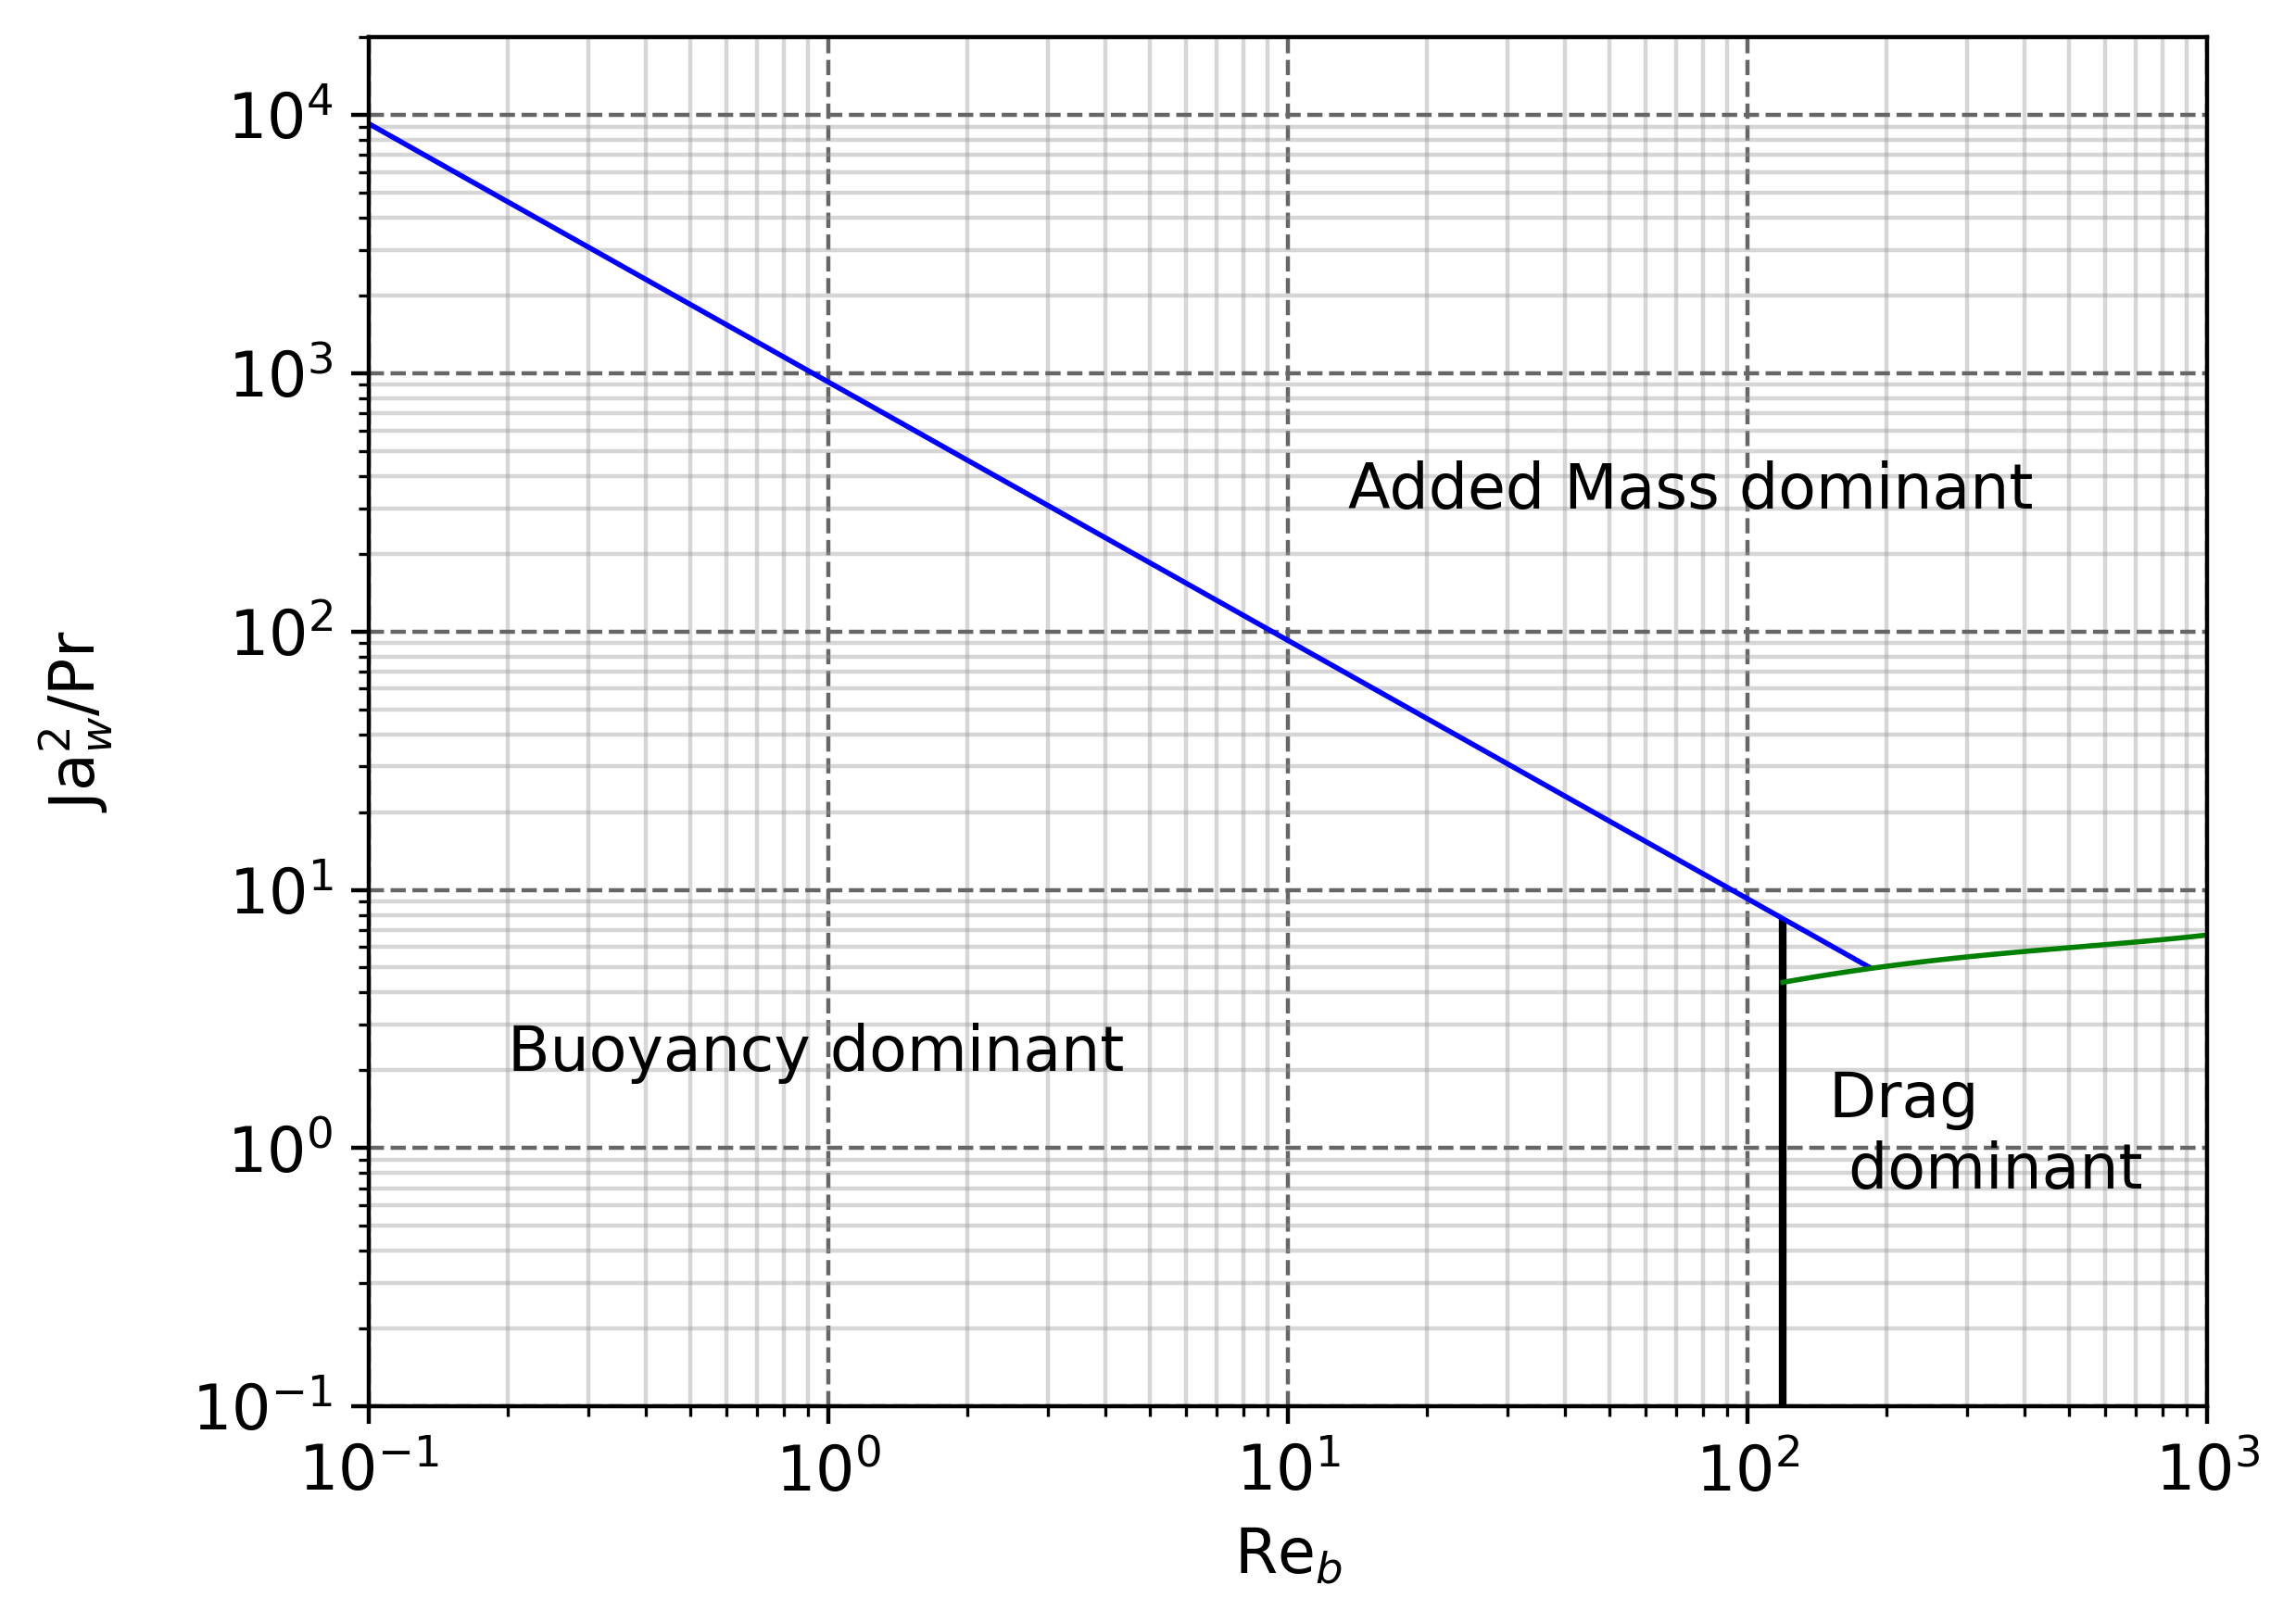
\includegraphics[width=0.49\linewidth]{img/forces/map_1bar_bis.png}
\hfill
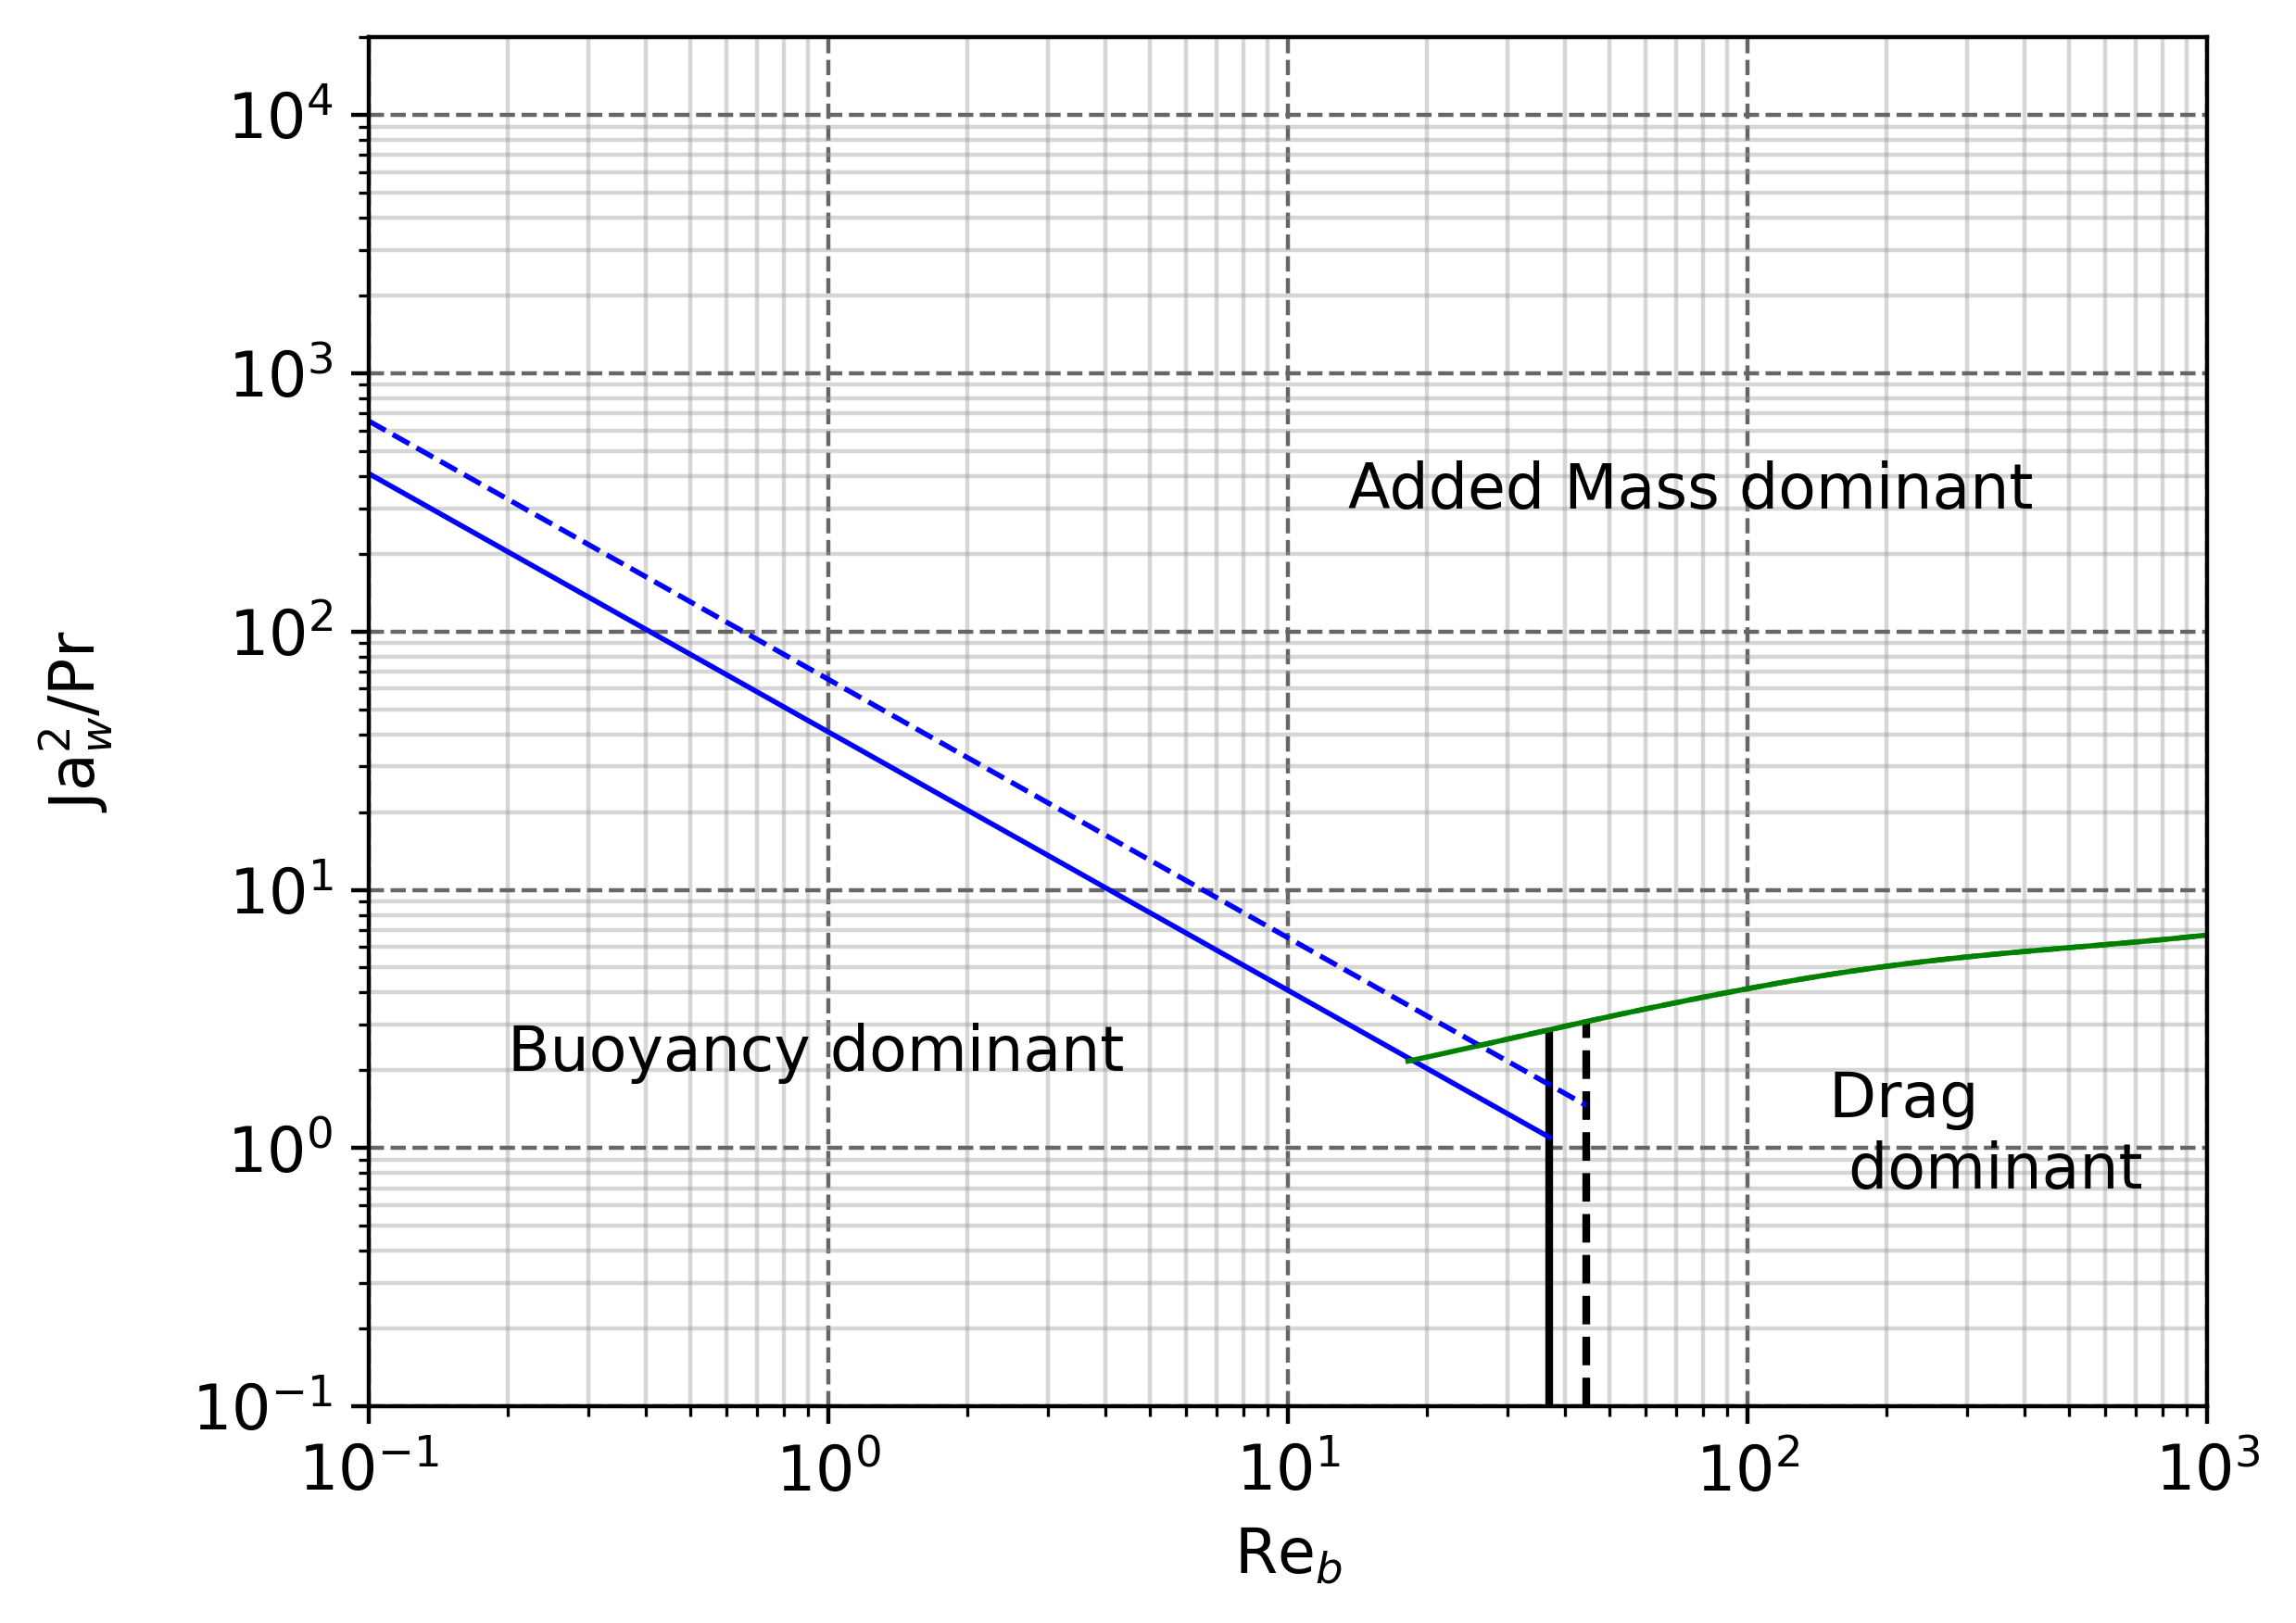
\includegraphics[width=0.49\linewidth]{img/forces/map_150bar_bis.png}
\caption{Force predominance map. Green, blue and black lines are respectively conditions (\ref{eq:AMvsD}),  (\ref{eq:AMvsB}) and (\ref{eq:DvsB}). Left represents $R=$0.25 mm for water at 1 Bar. Right represents $R=$0.05 mm, water at 150 Bar (plain lines) and R12 at 25 Bar (dashed lines).}
\label{fig:dom_slide}
\vspace{16pt}
\end{figure}

It appears that the increase in pressure along with the bubble diameter decrease leads to a larger range of flow parameters for which added mass effects and drag will be dominant. In addition, we also plotted the conditions for R12 at the similarity pressure of $26$ Bar where its properties such as $\We$ and $\rho_{L}/\rho_{V}$  are close to water in PWR conditions\cite{Garnier2001}. The proximity between the boundaries on Figure \ref{fig:dom_slide} interestingly indicates that \textit{bubbles in pressurized R12 tests are likely to behave very similarly to bubbles in PWR regarding their departure by sliding.}

It is also interesting to note that the frontier between added mass and drag defined by condition (\ref{eq:AMvsD}) remains unchanged for the different pressures, fluids and bubble radii.

\subsection{Application to Low Pressure Data}

In order to apply the predominance criteria, we gathered three data sets of experimental bubble departure diameter measurements in vertical flow boiling of water at atmospheric pressure. The associated experimental conditions are gathered on Table \ref{tab:exp_dd}. 

\vspace{16pt}
\begin{table}[!htb]
\centering
\caption{Thermal-hydraulics parameters range for the low pressure data.}
\vspace{14pt}
\begin{tabular}{|c||c|c|c|c||c|c|} \hline
Author &  $D_{h}$ (mm) & $G$ ($\debm$) & $\Delta T_{w}$ (K) & $D_{d}$ (mm)  & $\Re_{b}$ (-) & $\Ja_{w}^{2}/\Pr$ (-)\\
\hline
\hline
Sugrue \etal\cite{Sugrue2014} & 16.642 & 250 - 400 & 2 - 6 & 0.229 - 0.391 & 53.8 - 70.8 & 20.57 - 185.2 \\
\hline
Guan \etal\cite{Guan2014} & 9 & 87.3 - 319.2 & 4.5 - 8.5 & 0.62 - 1.85 & 75.9 - 406.02 & 104.2 - 371.6 \\
\hline
Maity\cite{Maity2000} & 20 & 0 - 239.6 & 5 - 5.9 & 0.788 - 1.713 & 0 - 241.04 & 128.6 - 179.06 \\
\hline
\end{tabular}
\label{tab:exp_dd}
\end{table}
\vspace{16pt}
To further justify the nearly-spherical shape hypothesis, we compute the range of Weber, Capillary and Eotvos numbers since they are representative of the deformability of the bubble under inertial, viscous and gravity effects (Table \ref{tab:exp_adim}).


\begin{table}[!htb]
\centering
\caption{Weber, Capillary and Eotvos numbers range for the low pressure data.}
\vspace{14pt}
\begin{tabular}{|c||c|c|c|}
\hline
Author & $\We$ (-) & $\Ca$ (-) & $\Eo$ (-)\\
\hline
\hline
Sugrue \etal\cite{Sugrue2014} & $6.36\times 10^{-3}$ - $12.6\times 10^{-3}$ & $2.22\times 10^{-4}$ - $3.64\times 10^{-4}$ & $2.09\times 10^{-3}$ - $6.09\times 10^{-3}$\\
\hline
Guan \etal\cite{Guan2014} & $3.79\times 10^{-3}$ - $82.8\times 10^{-3}$ & $0.998\times 10^{-4}$ - $4.93\times 10^{-4}$ & $1.53\times 10^{-2}$ - $13.6\times 10^{-2}$\\
\hline
Maity\cite{Maity2000} & $0$ - $3.5\times 10^{-2}$ & $0$ - $3.27 \times 10^{-4}$ & $2.48\times 10^{-2}$ - $11.7\times 10^{-2}$\\
\hline
\end{tabular}
\label{tab:exp_adim}
\end{table}
\vspace{16pt}


To compute the predominance boundaries as done in Figure \ref{fig:dom_slide}, we need to choose a bubble radius. Here we take the average departure radius of each data set to plot the associated boundaries. It appears that Guan and Maity data sets have very close average departure radius (approx. 0.6\ mm) and thus have the same predominance zones. The results are displayed on Figure \ref{fig:exp_dom}.
\begin{figure}[!htb]
\vspace{16pt}
\centering
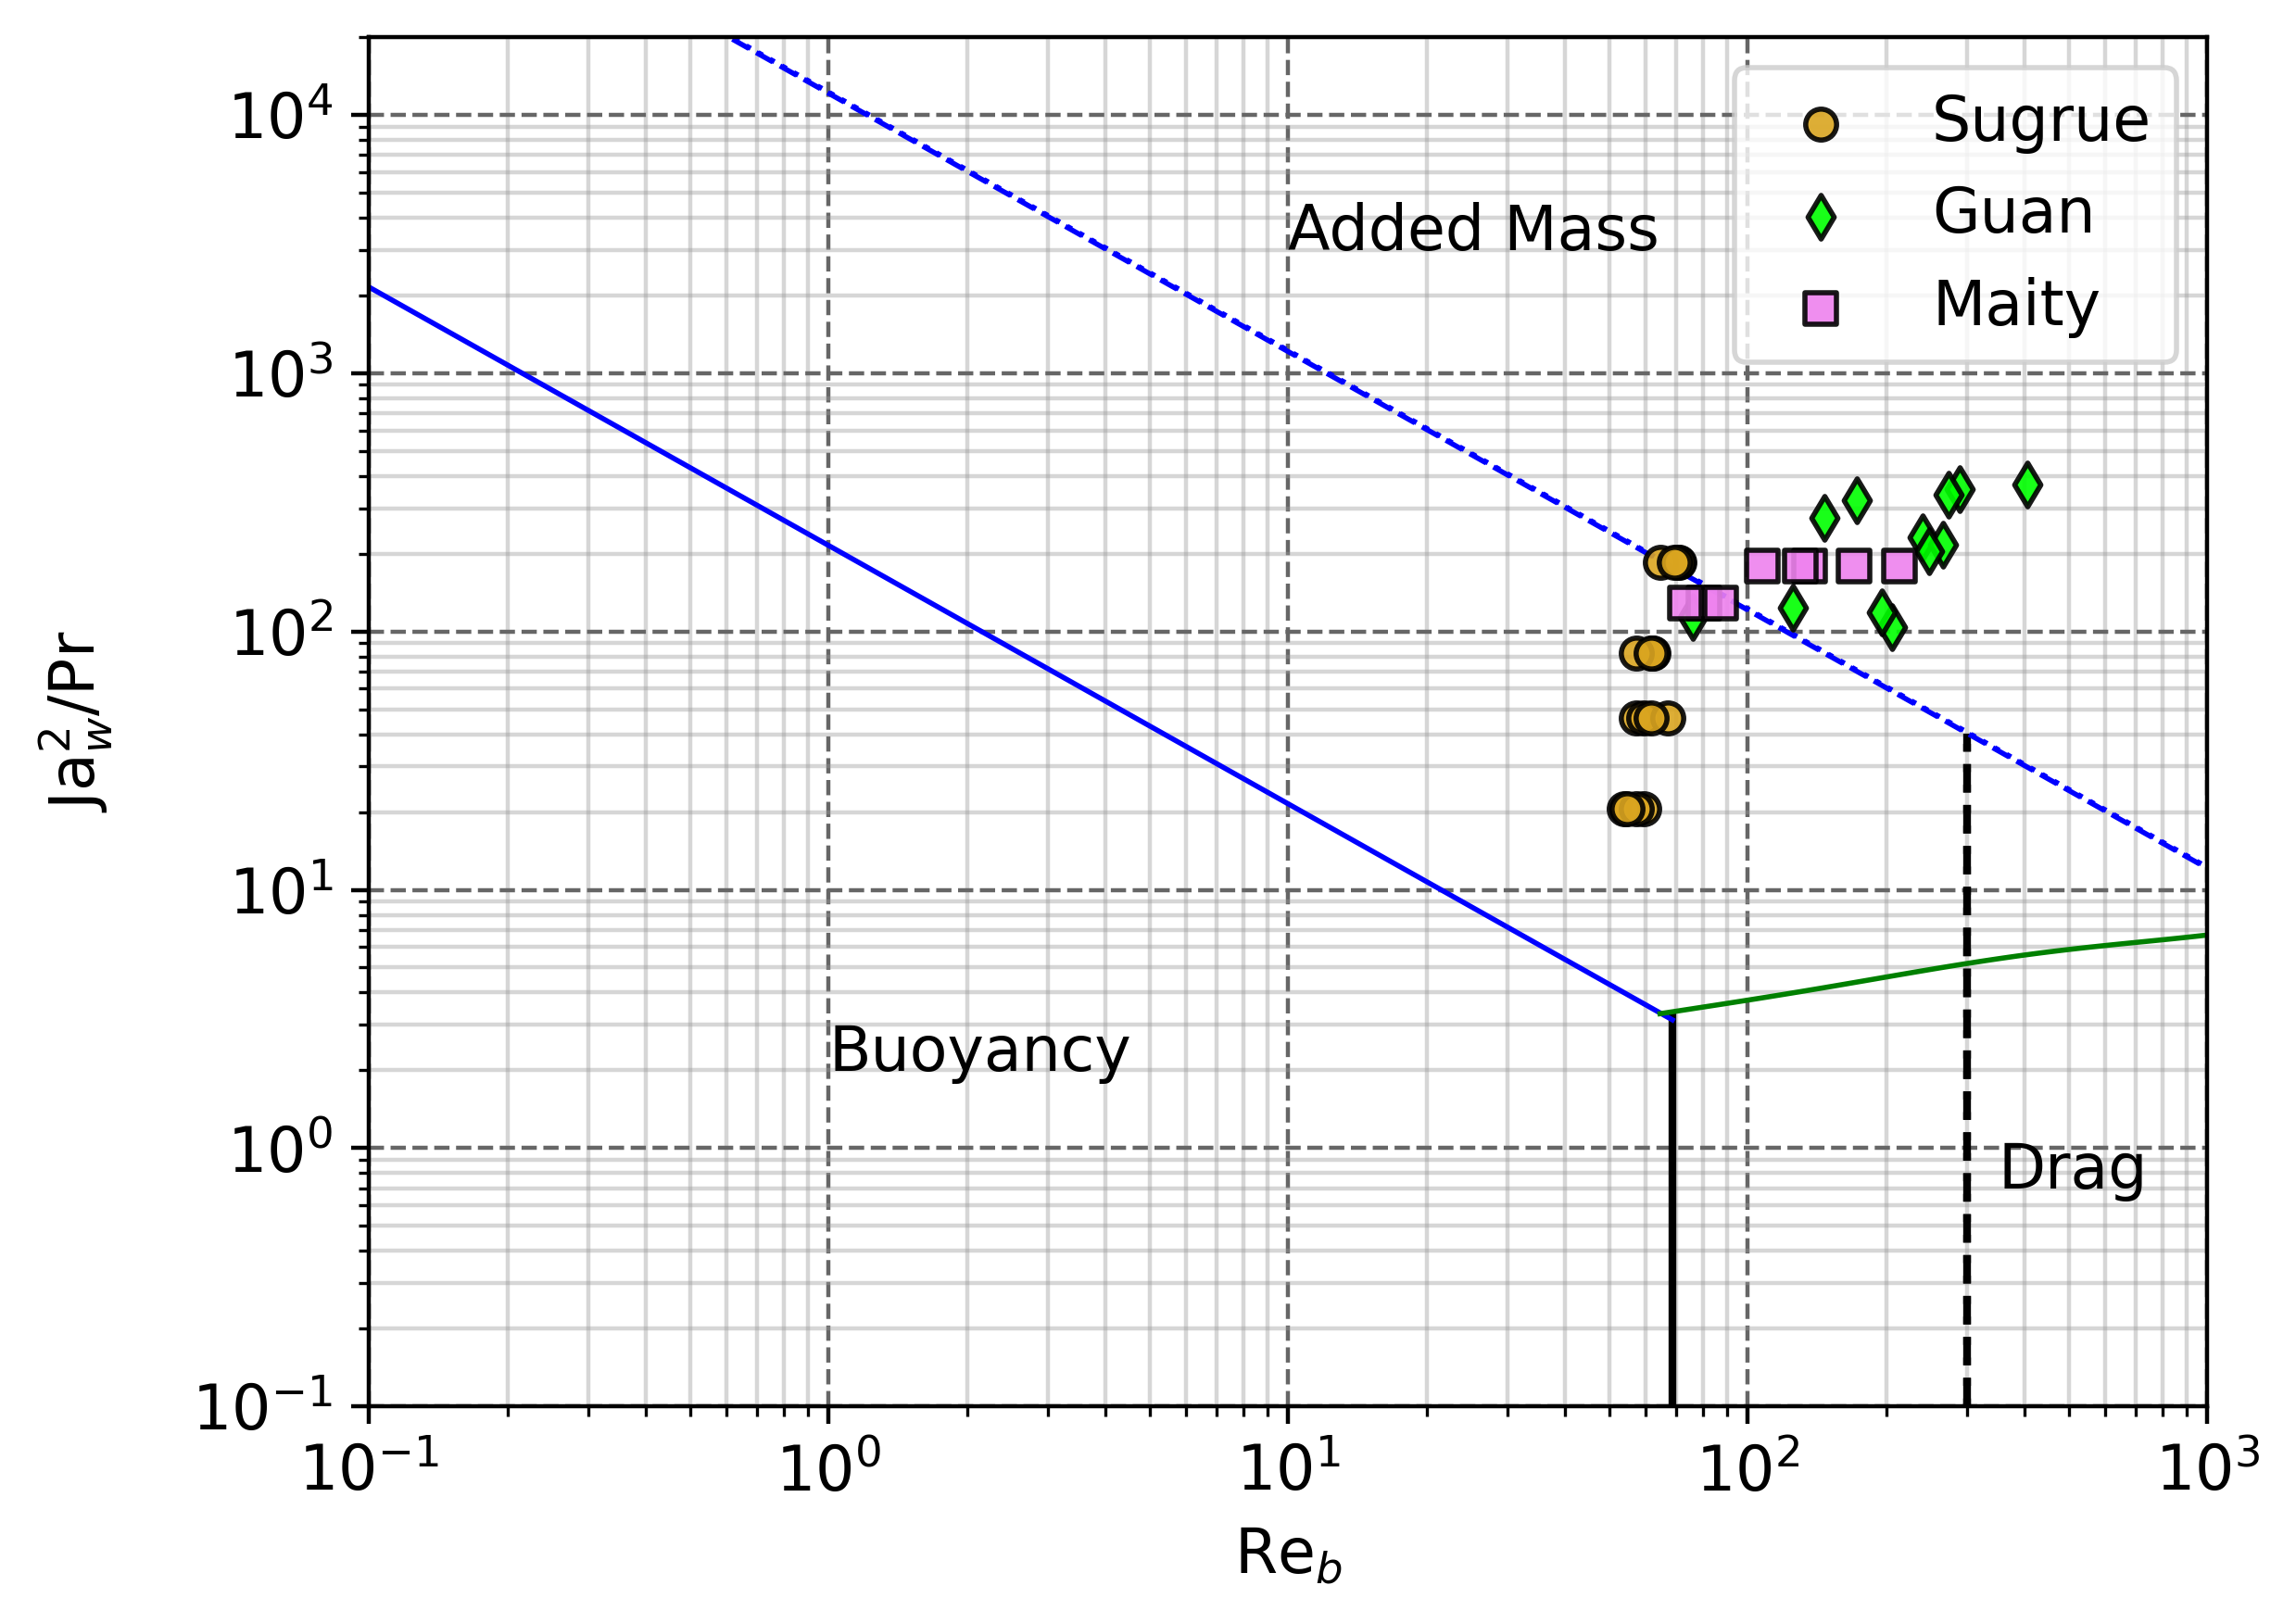
\includegraphics[width=0.6\linewidth]{img/forces/all_auth_map.png}
\caption{Experimental measurements in the dominance map. Plain lines correspond to Sugrue average departure radius (0.15 mm), dashed lines to Guan and Maity (0.59 mm).}
\label{fig:exp_dom}
\vspace{16pt}
\end{figure}

It immediately appears that when departure by sliding occurs, 32 measurements out of 37 seem to be dominated by added mass effects. The remaining 5 are buoyancy-dominant (Guan and Maity data) but placed really close to the added mass / buoyancy boundary on the map. This observation tends to indicates that at low pressure and mass fluxes, the departure by sliding could be triggered mostly by the added mass effects resulting of the coupling between the rapid initial bubble growth and the surrounding liquid velocity (Subsection \ref{subsec:AM}). 

This is mainly a consequence of the significant wall superheat reached in such boiling conditions along with high values of $\rho_{L}/\rho_{V}$, leading to high values of $\Ja_{w}^{2}/\Pr$. 


\subsection{Application to High Pressure Data}

Measurements of high-pressure bubble departure diameter are more difficult to find in the literature especially because of the great difficulty to provide clear visualization of individual bubbles when pressure increases, since bubbles are greatly reducing in size down to a few $\mu$m. 

Nevertheless, recent works such as those conducted by Kossolapov\cite{Kossolapov2021} have managed to conduct such measurements at pressures up to 39.8 Bar. To evaluate the forces responsible for sliding at higher pressures, closer to PWR operating conditions, we conduct the same analysis as we did with the low-pressure data. Experimental operations and non-dimensional numbers are summed up in Table \ref{tab:koss_exp}.

\begin{table}[!htb]
\centering
\caption{Thermal-hydraulics parameters and dimensionless numbers range for Kossolapov data.}
\vspace{14pt}
\begin{tabular}{|c||c|c|c|c||c|} \hline
Author &  $D_{h}$ (mm) & $G$ ($\debm$) & $P$ (Bar) & $D_{d}$ (mm)  & $\Re_{b}$ (-) \\
\hline
\hline
Kossolapov\cite{Kossolapov2021} & 11.78 & 500 - 2000 & 10.5 ; 19.9 ; 39.8 & 0.01 - 0.13 & 5.95 - 131.77\\
\hline
\end{tabular}
\vspace{14pt}
\begin{tabular}{|c|c|c|}
\hline
$\We$ (-) & $\Ca$ (-) & $\Eo$ (-)\\
\hline
\hline
$0.5\times 10^{-3}$ - $84.8\times 10^{-3}$ & $1.47\times 10^{-4}$ - $14.8\times 10^{-4}$ & $0.82\times 10^{-5}$ - $85\times 10^{-5}$\\
\hline
\end{tabular}
\label{tab:koss_exp}
\end{table}
\vspace{16pt}

Wall superheat or heat flux values are not specified in Kossolapov data because the given diameters were used to depict a global trend with pressure and mass flux. However, wall superheat at \textbf{Onset of Nucleate Boiling} can be roughly estimated using Frost \& Dzakowic correlation\cite{Frost1967} which yields approximately $\Delta T_{w}\approx $
4 K for water at $40$ Bar under a 1 MW/m$^{2}$ heat flux. To cover a tentatively large enough range of $\Ja_{w}^{2}/\Pr$ values, we will place the measurements from Kossolapov on the predominance map assuming three possible wall superheats : 1 K, 5 K and 10 K. 

The resulting map is displayed on Figure \ref{fig:koss_map}. In order to make it easier to interpret, we colored the stable added mass / drag boundary (\ref{eq:AMvsD}) in black and used 3 colors to distinguish between the three operating pressures. The arbitrary superheat are made distinct with the markers shapes.

\begin{figure}[!htb]
\vspace{16pt}
\centering
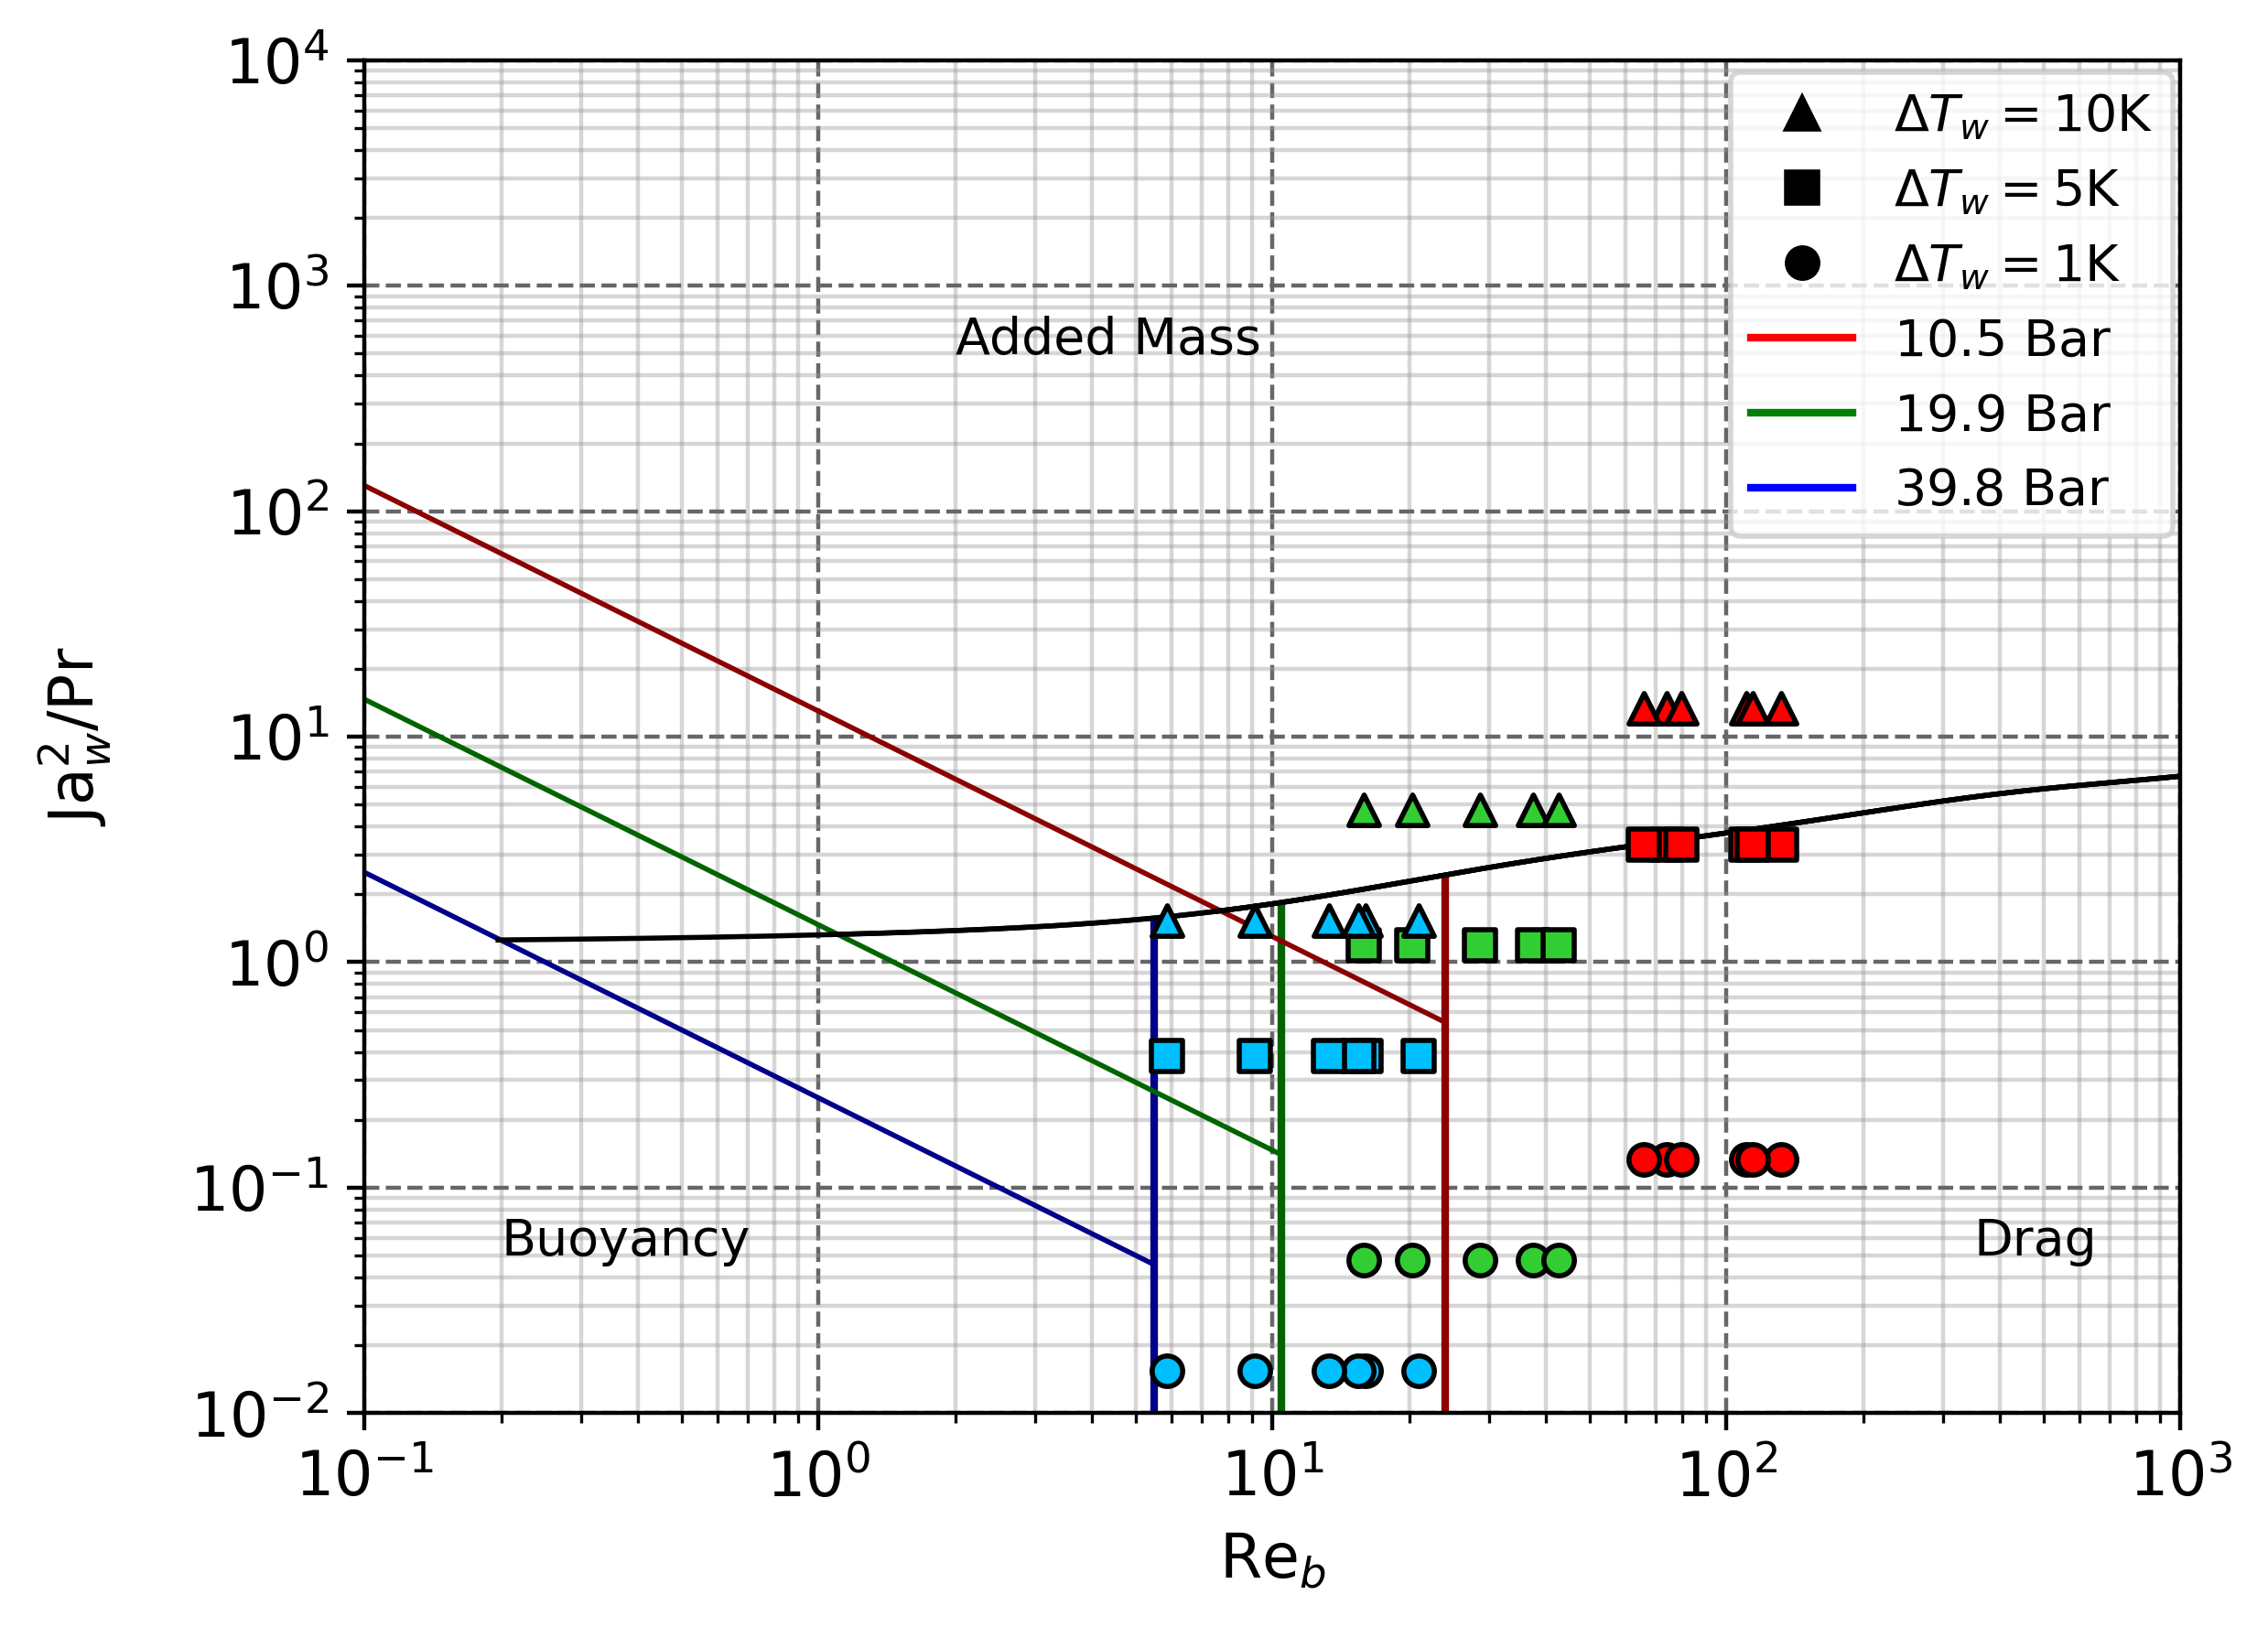
\includegraphics[width=0.6\linewidth]{img/forces/Koss_HP.png}
\caption{Experimental measurements from Kossolapov in the dominance map. Frontiers are plotted for the average departure radius at the given pressure. Blue : 39.8 Bar - Green : 19.9 Bar - Red : 10.5 Bar.}
\label{fig:koss_map}
\vspace{16pt}
\end{figure}

The main observation here relates to the values of $\Ja_{w}^{2}/\Pr$ which appear to be way smaller compared to the low pressure data, even for superheats as high as $10$K. This is mainly resulting from the strong decrease in the $\rho_{L}/\rho_{V}$ ratio with pressure, thus leading to predominance ranges where the force mostly responsible for departure by sliding is the drag. The higher mass fluxes also tend to increase this effect. Added mass only start to be significant under the 10 K superheat assumption.
%Moreover, we can note that the triangle-shaped zone corresponding to no clear dominance of one force against the other enlarges as the pressure increases.

Finally, this analysis of high pressure data tends to indicate that \emph{departure by sliding at high pressure is triggered in significantly different dynamic conditions in term of forces ratio (drag dominant) compared to low pressure (added mass dominant)}.

\section{Prediction of bubble departure diameter}
\label{sec:dd_pred}

The main goal of such a study would still remain to find a way to predict the departure diameter of bubbles in vertical flow boiling. Since only the capillary force is opposed to bubble departure, we can use non-dimensional force balance (\ref{eq:adim_bdf}) to search the maximum diameter above which :
\begin{equation}
 C_{AM,x}K^{2}\frac{\Ja_{w}^{2}}{\Pr}+\frac{\Re_{b}}{\Fr} + \frac{3}{8}C_{D}\Re_{b} > \frac{3}{2}\frac{f_{C,x}}{\Ca}
\label{eq:adim_dd}
\end{equation}

To compute $\Re_{b}$ and $C_{D}$, we use Reichardt's law\cite{Reichardt1951} for the wall liquid velocity and shear at a distance $y=R$. Diameters predictions results are displayed on Figure \ref{fig:pred_dd}. The supposed wall superheat for Kossolapov data is 1 K.

\begin{figure}[!htb]
\vspace{16pt}
\centering
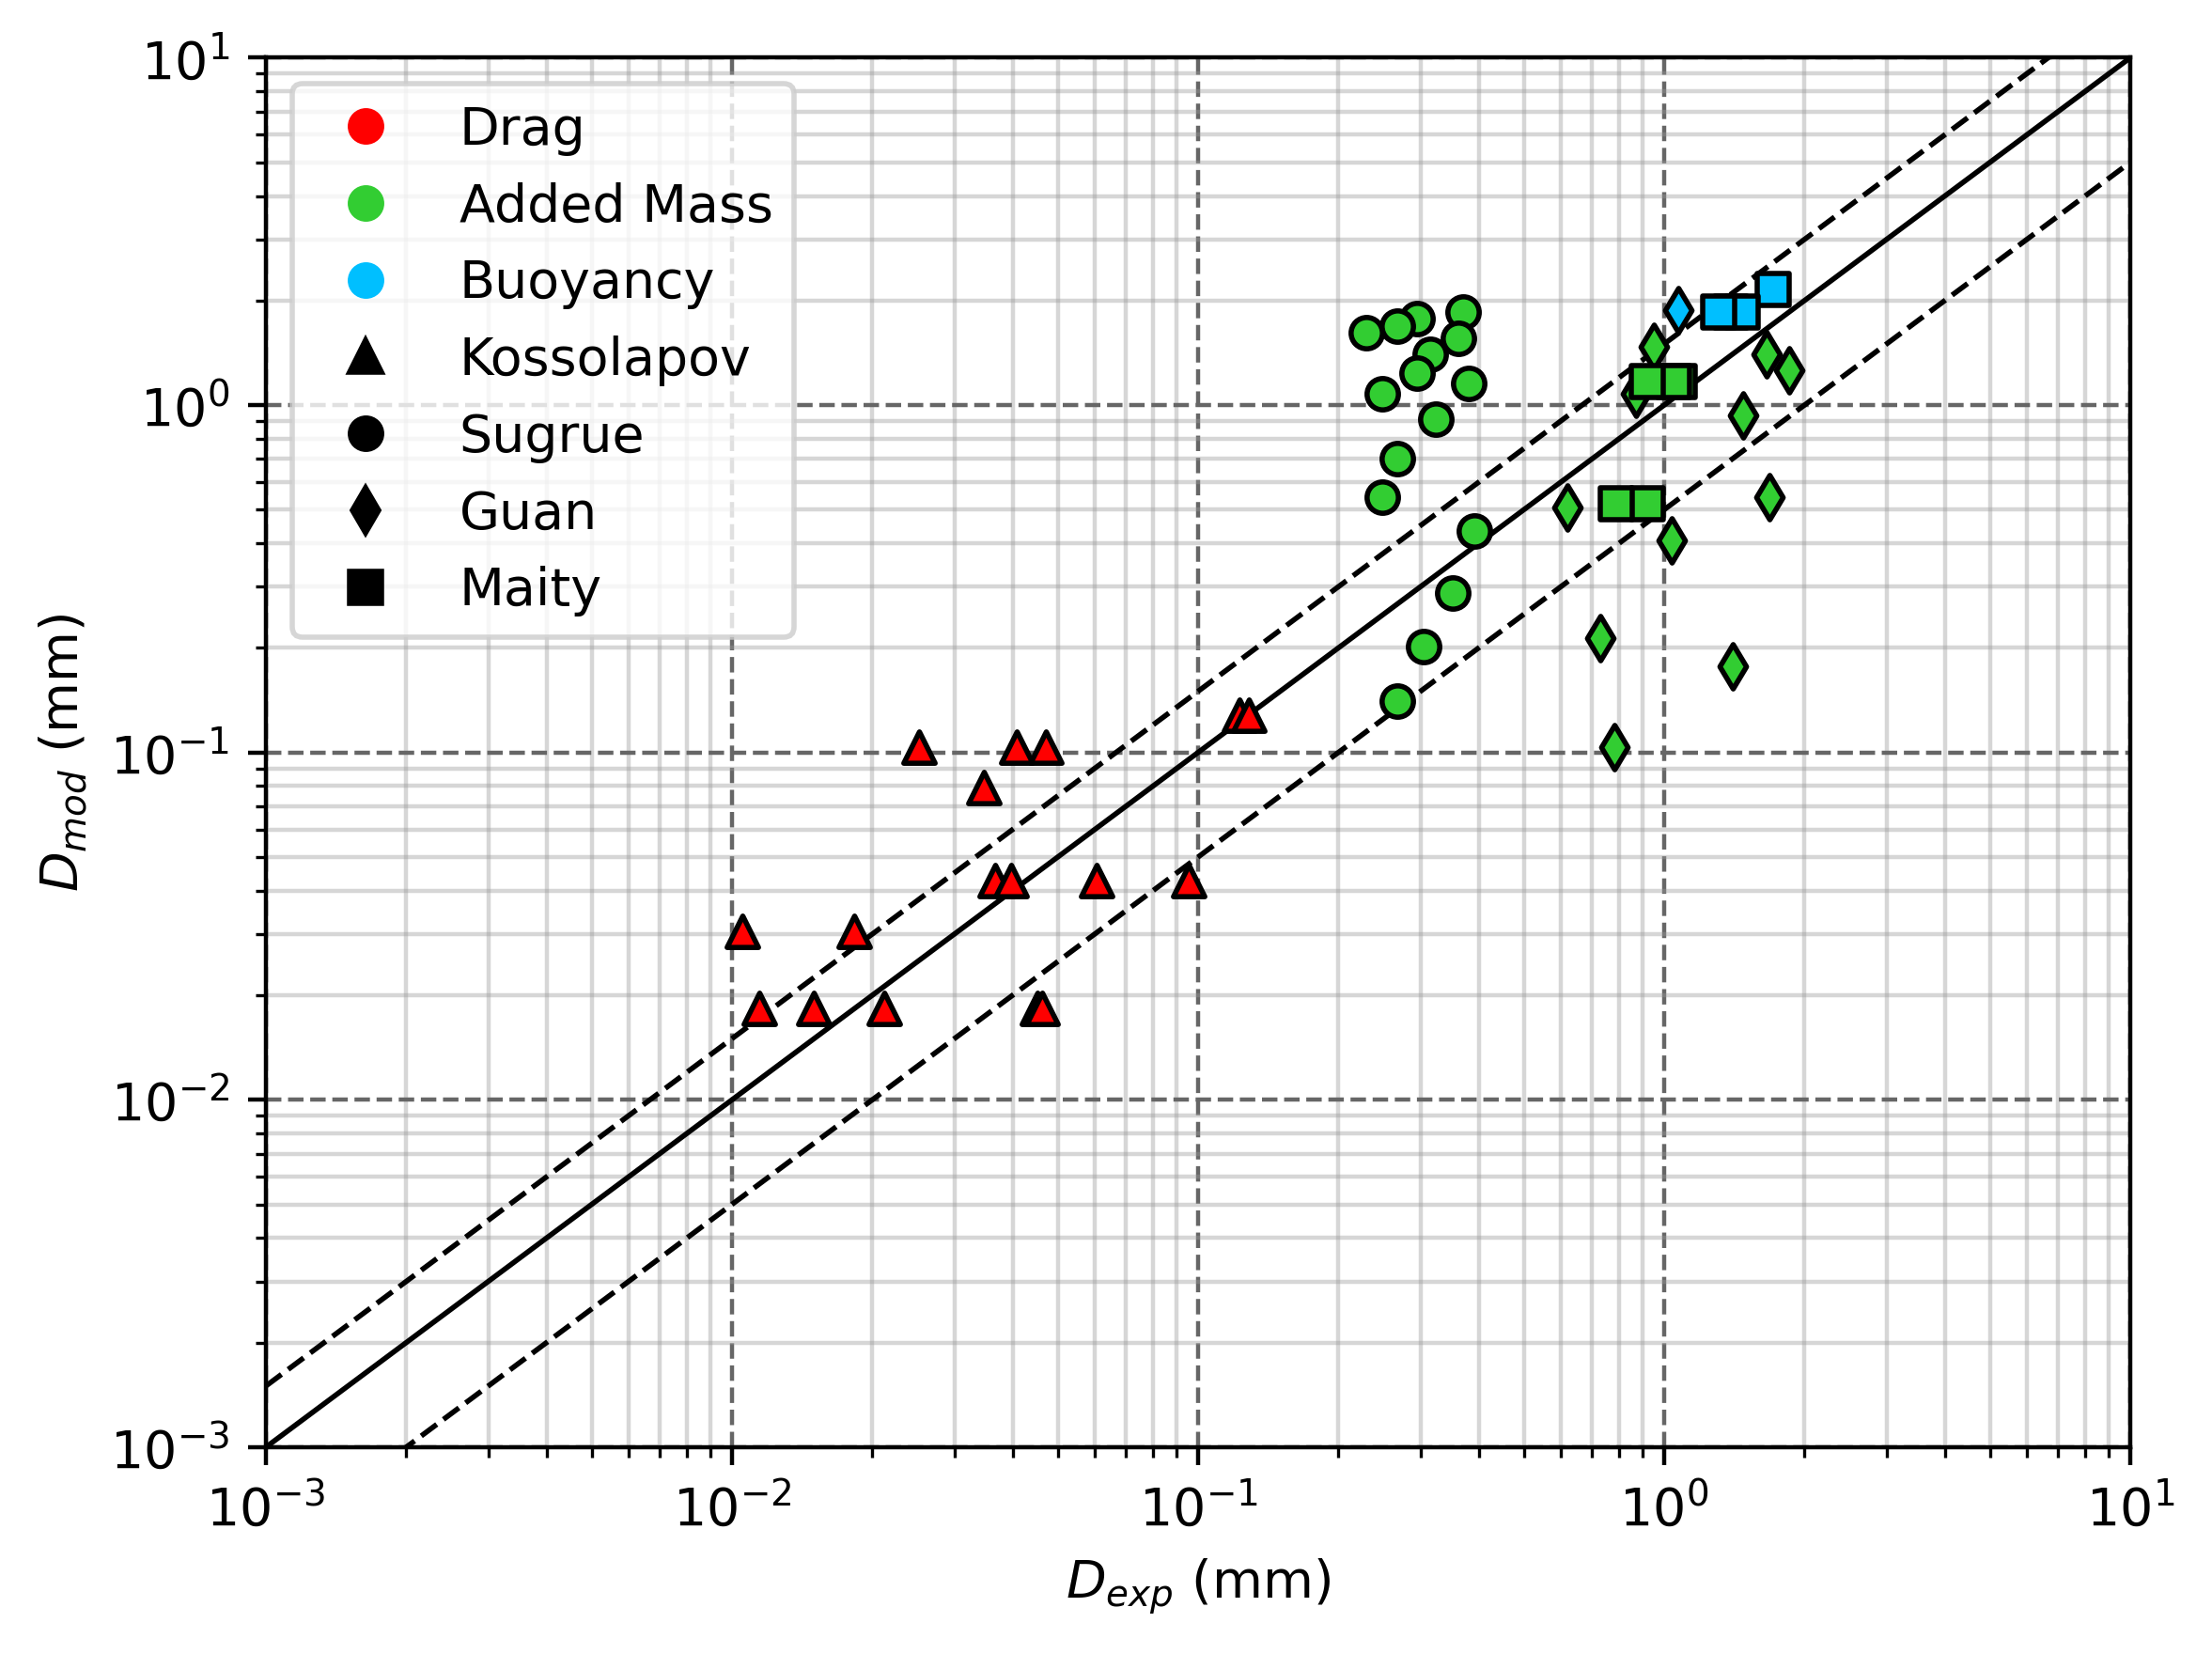
\includegraphics[width=0.49\linewidth]{img/forces/pred_dd_dom.png}
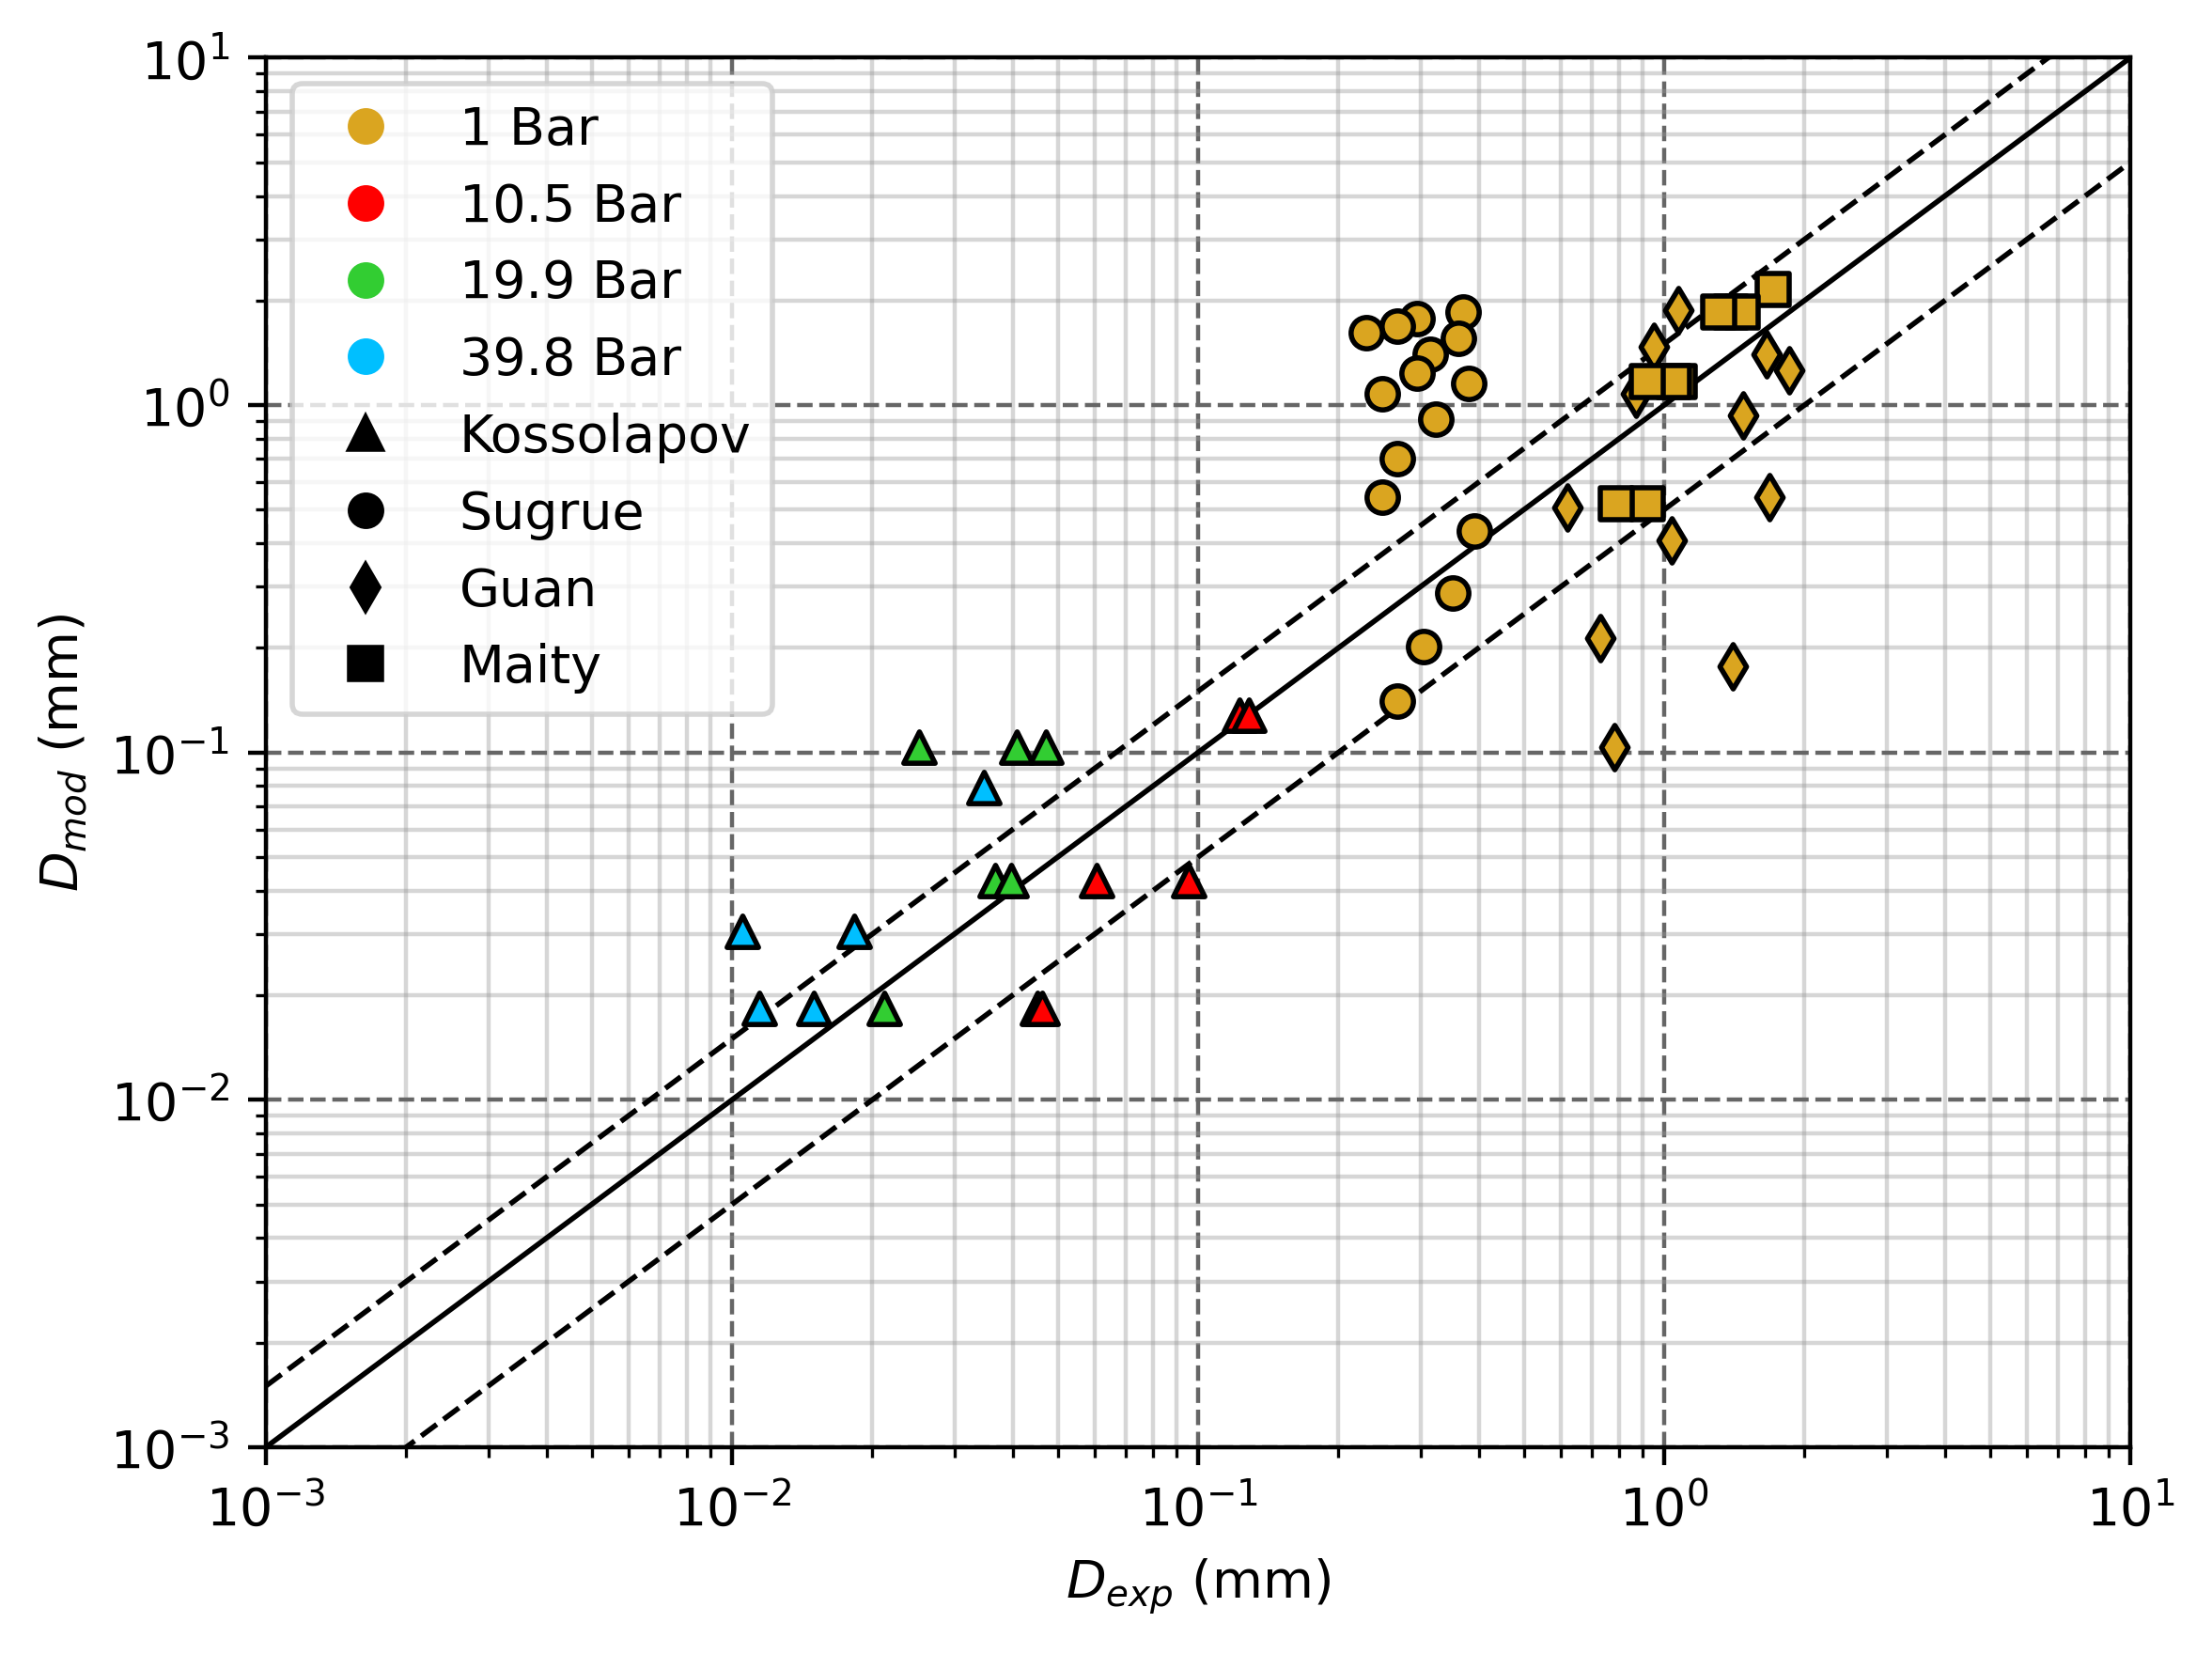
\includegraphics[width=0.49\linewidth]{img/forces/pred_dd_p.png}
\caption{Predicted diameter by Eq. \ref{eq:adim_dd} vs. experimental measurements. Colors refer to the dominant force at the departure by sliding (left) or to the operating pressure (right). $\pm 50\%$ error lines in dashed black.}
\label{fig:pred_dd}
\vspace{16pt}
\end{figure}

We can see that the predicted diameters seem to reasonably follow the global trend with pressure, which is an important feature in order to distinguish the different dynamic regimes depending on the flow conditions. 

The average contact and hysteresis angle used in the computations are $\theta=45\degree$, $\dtheta=36\degree$ for Sugrue's data (maximum hysteresis observed in her experiments) yielding an average error of 230.4\% ; $\theta=53\degree$, $\dtheta=27\degree$ for Guan's data (maximum hysteresis measured, accounting for uncertainties) yielding an average error of 182\% ; $\theta=60\degree$, $\dtheta=20\degree$ for Maity's data (average static angle, but increased hysteresis compared to the measurements) for an average error of 29.2\% ; $\theta=45\degree$, $\dtheta=1\degree$ for Kossolapov's data for an average error of 53.8\% (no measurements available).

Although the results seem to follow a correct trend with pressure, the average error can still be considered high on some data compared to other models\cite{Klausner1993}. However, such models often chose arbitrary values for parameters like the bubble foot diameter ($d_{w}=D/15$)\cite{Mazzocco2018} or the contact, hysteresis and inclination angles. Recent studies emphasized that such assumptions were substiantially wrong\cite{Bucci2021}. Moreover, those models consider an opposite contribution of the added mass regarding departure which seems to be incorrect as discussed earlier (Subsection \ref{subsec:AM}).

In this work, we insisted on keeping straight assumptions of a quasi-spherical bubble and to tried to apply the resulting laws for departure diameter prediction. \textbf{The only hypothetically free parameters were the average contact angle and hysteresis.} We tried to use author's data when available as inputs in our model. However, we did not have such measurements for Kossolapov's data and thus chose an average contact angle close to water FTO static contact angle (heater material used in his experiments) along with a very small hystersis, since very small bubbles in highly pressurized flow will be likely to keep non-deformed shapes because of surface tension effects getting stronger as the bubble diminishes in size. Moreover, we had to set a wall superheat which we chose to be $1$K (strongly drag-dominant regime).

Concerning the low pressure data, we observed that better results were obtained on Maity's measurements when using a bigger hysteresis angle. This may originate from the bubble foot diameter modeling, which was observed to be lower than the associated truncated sphere foot diameter in his experiments. In addition, the three low pressure data sets (Table \ref{tab:exp_dd}) have very close flow conditions, but significantly different measured departure diameter, especially when comparing Sugrue to Guan and Maity. The observed differences in experimental measurements can thus originate from the heater material, which impact is only indirectly included through the contact angle and hysteresis. This can explain the over-estimation of departure diameter on Sugrue's data when good agreement is observed with Guan and Maity. The same goes for the under-estimated diameters on Guan's data when we have a good agreement with Sugrue's measurements, explaining the high average relative deviation on those data sets.

\cleardoublepage % Empty page before the start of the next part


\part{Towards the Industrial Geometry}
% Chapter 1

\chapter{Promoteur} % Chapter title

\label{ch:promoteur} % For referencing the chapter elsewhere, use \autoref{ch:introduction} 




\section{Boiling freon in a tube with mixing vanes : DEBORA-Promoteur experiments}
\label{sec:deb_prom}

In this section, we simulate upward boiling flows of R12 in a vertical tube equipped with mixing vanes and compare the outlet void fraction profile predicted by NEPTUNE\_CFD with measurements coming from the DEBORA-Promoteur experiment.

\subsection{Description of the experiment}

In 2003, the wish to investigate boiling flows in complex geometries similar to those in PWR fuel assembly lead CEA and EDF to modify the DEBORA facility to introduce mixing vanes (MV) within the tube. This mixing device has been desgined to have the same geometric properties as the mixing vanes attached to rod bundle grids (Figure \ref{fig:promoteur}).

%
\begin{figure}[!htb]
\centering
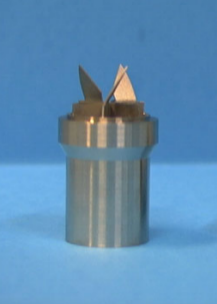
\includegraphics[height=4cm]{img/DEBORA-Promoteur/prom_pic.png}
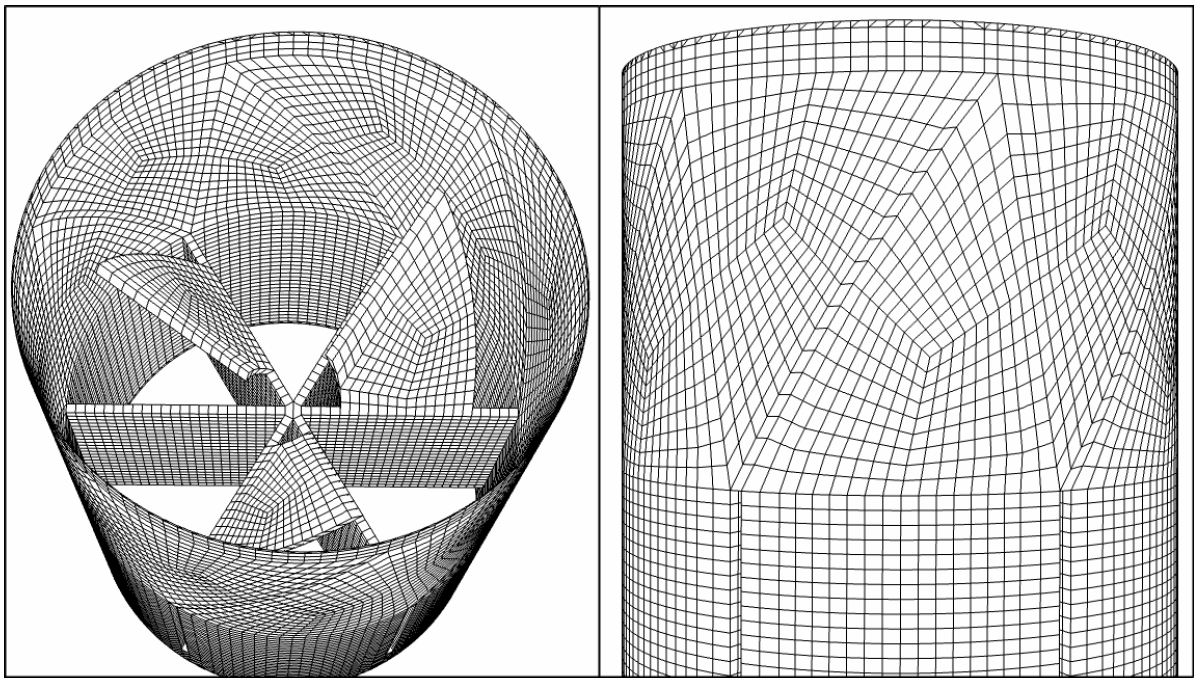
\includegraphics[height=4cm]{img/DEBORA-Promoteur/medium_mesh.PNG}
\caption{Picture of the mixing device (left) and its fine meshing (right).}
\label{fig:promoteur}
\end{figure}
%

Two series of measurements were conducted on this geometry : 

\begin{itemize}
\item Campaign 4800 : measurements of $\alpha$ using two optical probes, mixing device placed $0.455\text{m}\approx 23.5D_{h}$ upstream the end of the heating length
\item Campaign 5200 : measurements of $\alpha$ and $U_{G,z}$ using two optical probes, mixing device placed $0.192\text{m}\approx 10D_{h}$ upstream the end of the heating length
\end{itemize}

The goal of those tests was to observe the impact of the mixing device on the void fraction profile. The induced rotation is expected to gather the bubbles at the center of the tube and enhance condensation for highly subcooled cases. Those expectations are confirmed when looking at experimental $\alpha$ profiles on Figure \ref{fig:sim_prom}. The strong differences compared to simple tube profiles could explain the gain on the CHF value in PWR thanks to the mixing grids. Cases are named following the same nomenclature as presented in Section \ref{sec:debora}.

\subsection{NEPTUNE\_CFD simulations of DEBORA-Promoteur cases}

We simulated 3 cases for each position of the mixing device, covering different local thermodynamic quality near the vanes ($x_{eq,MV}$) :

\begin{itemize}
\item 48G3P26W23Te65 \& 52G3P26W23Te65 with $x_{eq,MV}\approx -1\%$ 
\item 48G3P26W23Te69 \& 52G3P26W23Te69 with $x_{eq,MV}\approx 4\%$ 
\item 48G3P26W23Te75 \& 52G3P26W23Te75 with $x_{eq,MV}\approx 12\%$ 
\end{itemize}

Computations are conducted using two meshes for Te69 cases : a large one (M1) with $444~703$ cells and a fine one (M2) with $3~487~627$ cells. Results for void fraction profiles are shown on Figure \ref{fig:sim_prom}.


%
\begin{figure}[!htb]
\centering
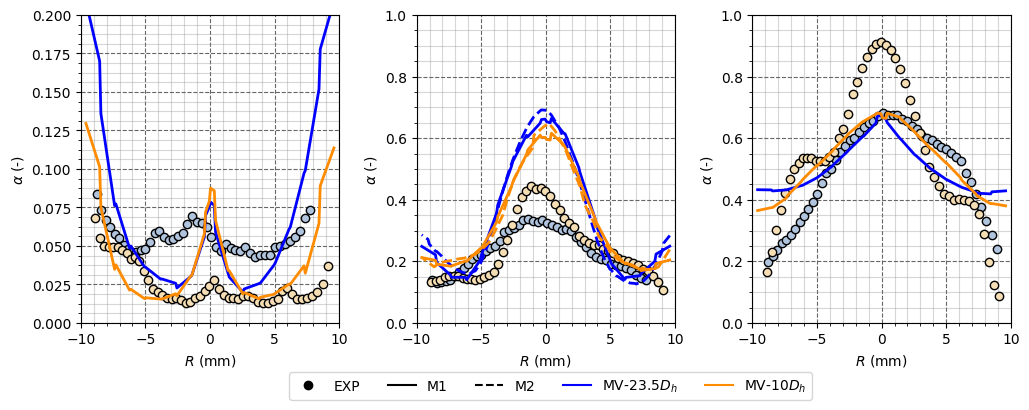
\includegraphics[scale=0.60]{img/DEBORA-Promoteur/alpha_prom.png}
\caption{NCFD (lines) vs. Exp. (circles) - $\alpha$ profiles for two MV positions (23.5$D_{h}$ in blue, $10D_{h}$ in orange) - $T_{in}=65\degree$C (left), $T_{in}=69\degree$C (middle), $T_{in}=75\degree$C (right) - Simulations using two meshes M1 (coarse) and M2 (fine) for $T_{in}=69\degree$C.}
\label{fig:sim_prom}
\end{figure}
%


Quantitatively speaking, it seems that NEPTUNE\_CFD reproduces the effect of vapor acculumation at the center thanks to the pressure gradient generated by the swirl induced by the mixing vanes. The radial position  of the core void fraction peak correctly matches the experimental one. 

However, measured void fraction profiles are not predicted correctly. A particularly strong overestimation of the core void fraction is observed as well as close to the wall. The CMFD results tend to rapidly reach a core void fraction around $60\%$ ($T_{in}=69\degree$C cases) and then flattens with increasing temperature ($T_{in}=75\degree$ cases). This contradicts experimental observation where the void fraction profile globally rises when inlet temperature increases, except at the wall where no peak is observed due to bubble removing effect by the liquid's rotation. Moreover, the $T_{in}=75\degree$ case with MV at $10D_{h}$ experimentally shows local $\alpha$ peaks at $R\approx \pm 6$mm which remain currently unexplained and not reproduced by the simulations. 

To investigate what could be a potential origin for the core void fraction peak overestimation, we present in Section \ref{sec:agate} single-phase flow simulations in the MV geometry.


\section{Liquid water flow in a tube with mixing vanes : AGATE-PROMOTEUR experiment}
\label{sec:agate}

In this penultimate section, we briefly investigate single-phase flow within the same geometry as Section \ref{sec:deb_prom}.

\subsection{Description of the experiment}

In 2003, using the same experimental geometry as DEBORA-Promoteur cases (Section \ref{sec:deb_prom}), Laser Doppler Velocimetry (LDV) measurements of velocity and turbulent fluctutations for an adiabatic single-phase flow of water were conducted. The outlet pressure was around $P=2$ bar with an inlet mass flux $G\approx 3000~\debm$. Measurements were conducted on $6$ different diameters and repeated at various axial positions upstream and downstream the mixing vanes.

A first look at experimental measurements (Figure \ref{fig:agate1}) shows that the vanes geometry induces significantly non-symmetric velocity profile. Moreover, we observe high turbulent fluctuations which maximum is located at the same radial position as the maximum radial velocity gradient.

\subsection{NEPTUNE\_CFD simulations of AGATE-Promoteur case}

On Figure \ref{fig:agate1}, we present some of the results obtained with NEPTUNE\_CFD using the $R_{ij}-\varepsilon~SSG$ turbulence model on the M2 mesh, along with a smooth wall law and a rough wall law (roughness $\epsilon=0.01$mm). The turbulent fluctuations Root Mean Square (RMS) correspond, for instance, to $\sqrt{<u^{'^{2}}_{x}>}$ for the $x$ direction where $u'_{i}$ represents the fluctuating part of the velocity along compononent $i$ and $<.>$ the time-averaging operator. Subscripts $R$ and $A$ stand for radial and axial values ; $U_{0}$ is the average inlet velocity.


%
\begin{figure}[!htb]
\centering
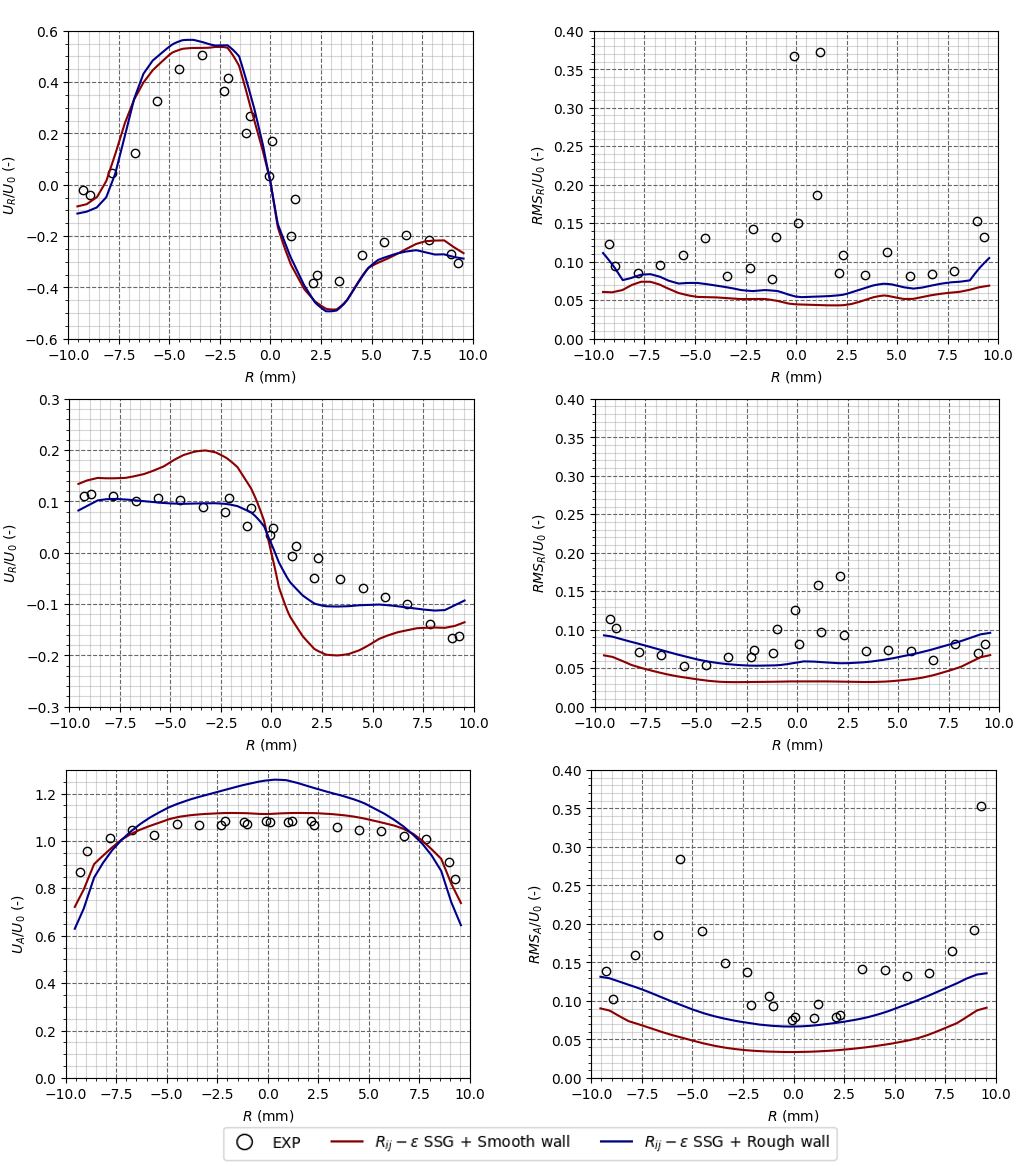
\includegraphics[scale=0.3]{img/AGATE/test.png}
\caption{NCFD vs. Exp. - Top \& Middle : Radial velocity and turbulent RMS ($z=30$mm \& $z=440$mm) -  Bottom : Axial velocity and turbulent RMS ($z=440$mm).}
\label{fig:agate1}
\end{figure}

Non-symmetric radial velocity profiles close to the MV are quite well reproduced by the simulations. However, far downstream the MV, it appears that the fluid's rotation is overestimated by the model with a smooth wall approach, while applying a roughness helps to reduce the magnitude of the swirl. Moreover, the radial turbulent fluctuations are better estimated by the rough wall approach at $z=440$~mm.

On the other hand, it seems that the rough wall approach deteriorates the axial velocity profile compared to the experiment. As shown on the bottom part of Figure \ref{fig:agate1}, the smooth wall simulation returns a flat velocity profile closer to the experiment than the rough wall one which overestimates the core velocity peak.

Both simulations globally underestimate the turbulent fluctuations, which can have a significant influence over the observed discrepancies on velocity profiles since turbulence plays a key role to homogenize the fluid flow. 

Those results finally highlight the fact that simulation of such rotating flows may need a particular wall approach to better capture the induced swirl and its dissipation. Correct prediction of turbulent fluctuations would be of significant interest to ensure liquid velocity validation. Further investigations on boiling cases could possibly be improved by a roughness approach, which is the current correction used for two-phase wall laws (Subsection \ref{subsec:wall_func}). 



\part{Conclusion} % First part of the thesis

%% Chapter 1

\chapter{Introduction} % Chapter title

\label{ch:introduction} % For referencing the chapter elsewhere, use \autoref{ch:introduction} 

%----------------------------------------------------------------------------------------

This template for \LaTeX\ has two goals:
\begin{enumerate}
\item Provide students with an easy-to-use template for their Master's or PhD thesis (though it might also be used by other types of authors for reports, books, etc.).
\item Provide a classic, high-quality typographic style that is inspired by \citeauthor{bringhurst:2002}'s ``\emph{The Elements of Typographic Style}'' \citep{bringhurst:2002}.
\marginpar{\myTitle \myVersion}
\end{enumerate}

The bundle is configured to run with a \emph{full} MiK\TeX\ or \TeX Live installation right away and, therefore, it uses only freely available fonts.

People interested only in the nice style and not the whole bundle can now use the style stand-alone via the file \texttt{classicthesis.sty}. This works now also with ``plain'' \LaTeX.

As of version 3.0, \texttt{classicthesis} can also be easily used with \mLyX\footnote{\url{http://www.lyx.org}} thanks to Nicholas Mariette and Ivo Pletikosi\'c. The \mLyX\ version of this manual will contain more information on the details.

This should enable anyone with a basic knowledge of \LaTeXe\ or \mLyX\ to produce beautiful documents without too much effort. In the end, this is my overall goal: more beautiful documents, especially theses, as I am tired of seeing so many ugly ones.

The whole template and the used style is released under the \textsmaller{GNU} General Public License. 

If you like the style then I would appreciate a postcard:
\begin{center}
André Miede \\
Detmolder Straße 32 \\
31737 Rinteln \\
Germany
\end{center}

\noindent The postcards I received so far are available at:
\begin{center}
 \url{http://postcards.miede.de}
\end{center}
\marginpar{A well-balanced line width improves the legibility of the text. That's what typography is all about, right?} So far, many theses, some books, and several other publications have been typeset successfully with it. If you are interested in some typographic details behind it, enjoy Robert Bringhurst's wonderful book. % \citep{bringhurst:2002}.

\paragraph{Important Note:} Some things of this style might look unusual at first glance, many people feel so in the beginning. However, all things are intentionally designed to be as they are, especially these:
\begin{itemize}
\item No bold fonts are used. Italics or spaced small caps do the job quite well.
\item The size of the text body is intentionally shaped like it is. It supports both legibility and allows a reasonable amount of information to be on a page. And, no: the lines are not too short.
\item The tables intentionally do not use vertical or double rules. See the documentation for the \texttt{booktabs} package for a nice discussion of this topic.\footnote{To be found online at \\ \url{http://www.ctan.org/tex-archive/macros/latex/contrib/booktabs/}.}
\item And last but not least, to provide the reader with a way easier access to page numbers in the table of contents, the page numbers are right behind the titles. Yes, they are \emph{not} neatly aligned at the right side and they are \emph{not} connected with dots that help the eye to bridge a distance that is not necessary. If you are still not convinced: is your reader interested in the page number or does she want to sum the numbers up?
\end{itemize}

\noindent Therefore, please do not break the beauty of the style by changing these things unless you really know what you are doing! Please.

\paragraph{Yet Another Important Note:} Since \texttt{classicthesis}' first release in 2006, many things have changed in the \LaTeX\ world.  Trying to keep up-to-date, \texttt{classicthesis} grew and evolved into many directions, trying to stay (some kind of) stable and be compatible with its port to \mLyX. However, there are still many remains from older times in the code, many dirty workarounds here and there, and several other things I am absolutely not proud of (for example my unwise combination of \acsfont{KOMA} and \texttt{titlesec} etc.). \graffito{An outlook into the future of \texttt{classicthesis}.}

Currently, I am looking into how to completely re-design and re-implement \texttt{classicthesis} making it easier to maintain and to use. As a general idea, \texttt{classicthesis.sty} should be developed and distributed separately from the template bundle itself. Excellent spin-offs such as \texttt{arsclassica} could also be integrated (with permission by their authors) as format configurations. Also, current trends of \texttt{microtype}, \texttt{fontspec}, etc. should be included as well. As I am not really into deep \LaTeX\ programming, I will reach out to the \LaTeX\ community for their expertise and help.

%----------------------------------------------------------------------------------------

\section{Organization}
A very important factor for successful thesis writing is the organization of the material. This template suggests a structure as the following:
\begin{itemize}
\marginpar{You can use these margins for summaries of the text body\dots}
\item\texttt{Chapters/} is where all the ``real'' content goes in separate files such as \texttt{Chapter01.tex} etc.
\item\texttt{FrontBackMatter/} is where all the stuff goes that surrounds the ``real'' content, such as the acknowledgments, dedication, etc.
\item\texttt{gfx/} is where you put all the graphics you use in the thesis. Maybe they should be organized into subfolders depending on the chapter they are used in, if you have a lot of graphics.
\item\texttt{Bibliography.bib}: the Bib\TeX\ database to organize all the references you might want to cite.
\item\texttt{classicthesis.sty}: the style definition to get this awesome look and feel. Bonus: works with both \LaTeX\ and \textsc{pdf}\LaTeX\dots and \mLyX.
\item\texttt{ClassicThesis.tcp} a \TeX nicCenter project file. Great tool and it's free!
\item\texttt{ClassicThesis.tex}: the main file of your thesis where all the content gets bundled together.
\item\texttt{classicthesis-config.tex}: a central place to load all nifty packages that are used. In there, you can also activate backrefs in order to have information in the bibliography about where a source was cited in the text (\ie, the page number).
    
\emph{Make your changes and adjustments here.} This means that you specify here the options you want to load \texttt{classicthesis.sty} with. You also adjust the title of your thesis, your name, and all similar information here. Refer to \autoref{sec:custom} for more information.

This had to change as of version 3.0 in order to enable an easy transition from the ``basic'' style to \mLyX.
\end{itemize}

\noindent In total, this should get you started in no time.

%----------------------------------------------------------------------------------------

\section{Style Options}\label{sec:options}

There are a couple of options for \texttt{classicthesis.sty} that allow for a bit of freedom concerning the layout: \marginpar{\dots or your supervisor might use the margins for some comments of her own while reading.}
\begin{itemize}
\item General:
\begin{itemize}
\item\texttt{drafting}: prints the date and time at the bottom of each page, so you always know which version you are dealing with. Might come in handy not to give your Prof. that old draft.
\end{itemize}
	
\item Parts and Chapters:
\begin{itemize}
\item\texttt{parts}: if you use Part divisions for your document, you should choose this option. (Cannot be used together with \texttt{nochapters}.)

\item\texttt{nochapters}: allows to use the look-and-feel with classes that do not use chapters, \eg, for articles. Automatically turns off a couple of other options: \texttt{eulerchapternumbers}, \texttt{linedheaders}, \texttt{listsseparated}, and \texttt{parts}. 

\item\texttt{linedheaders}: changes the look of the chapter headings a bit by adding a horizontal line above the chapter title. The chapter number will also be moved to the top of the page, above the chapter title.
\end{itemize}

\item Typography:
\begin{itemize}
\item\texttt{eulerchapternumbers}: use figures from Hermann Zapf's Euler math font for the chapter numbers. By default, old style figures from the Palatino font are used.

\item\texttt{beramono}: loads Bera Mono as typewriter font. (Default setting is using the standard CM typewriter font.)

\item\texttt{eulermath}: loads the awesome Euler fonts for math. (Palatino is used as default font.)

\item\texttt{pdfspacing}: makes use of pdftex' letter spacing capabilities via the \texttt{microtype} package.\footnote{Use \texttt{microtype}'s \texttt{DVIoutput} option to generate DVI with pdftex.} This fixes some serious issues regarding math formul\ae\ etc. (\eg, ``\ss'') in headers. 

\item\texttt{minionprospacing}: uses the internal \texttt{textssc} command of the \texttt{MinionPro} package for letter spacing. This automatically enables the \texttt{minionpro} option and overrides the \texttt{pdfspacing} option.
\end{itemize}  

\item Table of Contents:
\begin{itemize}
\item\texttt{tocaligned}: aligns the whole table of contents on the left side. Some people like that, some don't.

\item\texttt{dottedtoc}: sets pagenumbers flushed right in the table of contents.

\item\texttt{manychapters}: if you need more than nine chapters for your document, you might not be happy with the spacing between the chapter number and the chapter title in the Table of Contents. This option allows for additional space in this context. However, it does not look as ``perfect'' if you use \verb|\parts| for structuring your document.
\end{itemize}

\item Floats:
\begin{itemize}
\item\texttt{listings}: loads the \texttt{listings} package (if not already done) and configures the List of Listings accordingly.
    
\item\texttt{floatperchapter}: activates numbering per chapter for all floats such as figures, tables, and listings (if used).	
    
\item\texttt{subfig}(\texttt{ure}): is passed to the \texttt{tocloft} package to enable compatibility with the \texttt{subfig}(\texttt{ure}) package. Use this option if you want use classicthesis with the \texttt{subfig} package.

\end{itemize}    

\end{itemize}

\noindent The best way to figure these options out is to try the different possibilities and see, what you and your supervisor like best.

In order to make things easier in general, \texttt{classicthesis-config.tex} contains some useful commands that might help you.

%----------------------------------------------------------------------------------------

\section{Customization}\label{sec:custom}

This section will give you some hints about how to adapt \texttt{classicthesis} to your needs.

The file \texttt{classicthesis.sty} contains the core functionality of the style and in most cases will be left intact, whereas the file \texttt{classic\-thesis-config.tex} is used for some common user customizations. 

The first customization you are about to make is to alter the document title, author name, and other thesis details. In order to do this, replace the data in the following lines of \texttt{classicthesis-config.tex:}\marginpar{Modifications in \texttt{classic\-thesis-config.tex}
}

\begin{lstlisting}
\newcommand{\myTitle}{A Classic Thesis Style\xspace}
\newcommand{\mySubtitle}{An Homage to ...\xspace}
\end{lstlisting}

Further customization can be made in \texttt{classicthesis-config.tex} by choosing the options to \texttt{classicthesis.sty} (see~\autoref{sec:options}) in a line that looks like this:

\begin{lstlisting}
\PassOptionsToPackage{eulerchapternumbers,listings,drafting, pdfspacing, subfig,beramono,eulermath,parts}{classicthesis}
\end{lstlisting}

Many other customizations in \texttt{classicthesis-config.tex} are possible, but you should be careful making changes there, since some changes could cause errors.

Finally, changes can be made in the file \texttt{classicthesis.sty}, \marginpar{Modifications in \texttt{classicthesis.sty}} although this is mostly not designed for user customization. The main change that might be made here is the text-block size, for example, to get longer lines of text.

%----------------------------------------------------------------------------------------

\section{Issues}\label{sec:issues}
This section will list some information about problems using \texttt{classic\-thesis} in general or using it with other packages.

Beta versions of \texttt{classicthesis} can be found at Bitbucket:
\begin{center}
    \url{https://bitbucket.org/amiede/classicthesis/}
\end{center}
There, you can also post serious bugs and problems you encounter.

\subsection*{Compatibility with the \texttt{glossaries} Package}
If you want to use the \texttt{glossaries} package, take care of loading it with the following options:
\begin{verbatim}
\usepackage[style=long,nolist]{glossaries}
\end{verbatim}

\noindent Thanks to Sven Staehs for this information. 

\subsection*{Compatibility with the (Spanish) \texttt{babel} Package}
Spanish languages need an extra option in order to work with this template:
\begin{lstlisting}
    \usepackage[spanish,es-lcroman]{babel}
\end{lstlisting}
Thanks to an unknown person for this information (via the issue reporting). 

\paragraph{Further information for using \texttt{classicthesis} with Spanish (in addition to the above)}
In the file \texttt{ClassicThesis.tex} activate the language: 
\begin{lstlisting}
    \selectlanguage{spanish}
\end{lstlisting}

If there are issues changing \verb|\tablename|, \eg, using this:
\begin{lstlisting}
    \renewcommand{\tablename}{Tabla}
\end{lstlisting}

This can be solved by passing \texttt{es-tabla} parameter to \texttt{babel}:
\begin{lstlisting}
    \PassOptionsToPackage{es-tabla,spanish,es-lcroman,english}{babel}
    \usepackage{babel}
\end{lstlisting}

But it is also necessary to set \texttt{spanish} in the \verb|\documentclass|.

Thanks to Alvaro Jaramillo Duque for this information. 

\subsection*{Compatibility with the \texttt{pdfsync} Package}
Using the \texttt{pdfsync} package leads to linebreaking problems with the \texttt{graffito} command. Thanks to Henrik Schumacher for this information. 

%----------------------------------------------------------------------------------------

\section{Future Work}
So far, this is a quite stable version that served a couple of people well during their thesis time. However, some things are still not as they should be. Proper documentation in the standard format is still missing. In the long run, the style should probably be published separately, with the template bundle being only an application of the style. Alas, there is no time for that at the moment\dots it could be a nice task for a small group of \LaTeX nicians.

Please do not send me email with questions concerning \LaTeX\ or the template, as I do not have time for an answer. But if you have comments, suggestions, or improvements for the style or the template in general, do not hesitate to write them on that postcard of yours.

%----------------------------------------------------------------------------------------

\section{Beyond a Thesis}
The layout of \texttt{classicthesis.sty} can be easily used without the framework of this template. A few examples where it was used to typeset an article, a book or a curriculum vitae can be found in the folder \texttt{Examples}. The examples have been tested with \texttt{latex} and \texttt{pdflatex} and are easy to compile. To encourage you even more, PDFs built from the sources can be found in the same folder.

%----------------------------------------------------------------------------------------

\section{License}
\paragraph{GNU General Public License:} This program is free software; you can redistribute it and/or modify it under the terms of the \textsmaller{GNU} General Public License as published by the Free Software Foundation; either version 2 of the License, or (at your option) any later version.

This program is distributed in the hope that it will be useful, but \emph{without any warranty}; without even the implied warranty of \emph{merchantability} or \emph{fitness for a particular purpose}. See the \textsmaller{GNU} General Public License for more details. % Chapter 1

\cleardoublepage % Empty page before the start of the next part



%----------------------------------------------------------------------------------------
%	THESIS CONTENT - APPENDICES
%----------------------------------------------------------------------------------------

\appendix

\part{Appendix} % New part of the thesis for the appendix

% Appendix A

\chapter{Details on the Bubble Force Balance}

%----------------------------------------------------------------------------------------

\lipsum[13-14]


\begin{align}
r_{w} &= \frac{1}{2}\parth{\sin{\theta_{d}}R + \sin{\theta_{u}}R}\\
&= \frac{R}{2}\parth{ \sin{\theta_{s}+\dtheta} + \sin{\theta-\dtheta} }\\
&= \frac{R}{2}\crocht{2\sin{ \frac{\theta_{s}+\dtheta + \theta_{s}-\dtheta}{2} }\cos{ \frac{\theta_{s}+\dtheta - \parth{\theta_{s}-\dtheta}}{2}  }   } \\
&= R\sin{\theta_{s}}\cos{\dtheta}
\end{align}


\begin{align}
\vect{F_{CP}}&=\frac{2\sigma}{R_{c}}\frac{\pi d_{w}^{2}}{4}\vect{e_{y}}\\
&= \frac{2\sigma}{R}\frac{\pi 4R^{2}}{4}\sinsq{\theta}\cossq{\dtheta}\vect{e_{\bot}}\\
&=2\sigma \pi R \underbrace{\sinsq{\theta} \cossq{\dtheta}}_{f_{cp}}\vect{e_{\bot}}\\
&=2\pi R \sigma f_{cp}\parth{\theta, \dtheta}\vect{e_{\bot}}
\end{align}



\begin{align}
\vect{F_{CP}}\cdot \vect{e_{\bot}}&=-d_{w} \sigma \frac{\pi}{\alpha_{r}-\alpha_{u}}\parth{\cos{\alpha_{a}}- \cos{\alpha_{r}}}\\
&=\pi 2 R \sigma \frac{\sin{\alpha+\dalpha} + \sin{\alpha-\dalpha}}{2} \frac{\cos{\alpha+\dalpha} - \cos{\alpha-\dalpha}}{2\dalpha}   \\
&=2\pi R \sigma \frac{2\sin{\alpha}\cos{\dalpha}}{2}\frac{\parth{-2\sin{\alpha}\sin{\dalpha}}}{2\dalpha}\\
&=-2\pi R \sigma \underbrace{ \sinsq{\alpha}\frac{\sin{2\dalpha}}{2\dalpha} }_{f_{s,\bot}}\\
&=-2\pi R \sigma f_{s,\bot}\parth{\alpha,\dalpha}\\
\end{align}



\begin{align}
\vect{F_{s}}\cdot \vect{e_{\|}}&=-1.215d_{w}\sigma \frac{\pi\parth{\alpha_{r}-\alpha_{u}}}{\pi^{2}-\parth{\alpha_{r}-\alpha_{u}}^{2}}\parth{\sin{\alpha_{r}}+\sin{\alpha_{u}} }\\
&=-1.215 d_{w} \sigma \frac{\pi~2\dalpha}{\pi^{2}-4\dalpha^{2}}\parth{\sin{\alpha + \dalpha} + \sin{\alpha - \dalpha}}\\
&=-1.215  ~2R \sigma  \frac{\pi\dalpha}{\pi^{2}-4\dalpha^{2}}\parth{\sin{\alpha + \dalpha} + \sin{\alpha - \dalpha}}^{2}\\
&=-2\pi R \sigma \frac{1.215\dalpha}{\pi^{2}-4\dalpha^{2}}4\sinsq{\alpha}\cossq{\dalpha}\\
&=-2\pi R \sigma ~ \underbrace{ 1.215 \frac{\dalpha}{\parth{\frac{\pi}{2}}^{2}-\dalpha^{2}}\sinsq{\alpha}\cossq{\dalpha} }_{ f_{s,\|} }\\
&=-2\pi R \sigma f_{s,\|}\parth{\alpha,\dalpha}
\end{align}
%----------------------------------------------------------------------------------------

\section{Appendix Section Test}
\lipsum[15]

\graffito{More dummy text}
\lipsum[16]

%----------------------------------------------------------------------------------------

\section{Another Appendix Section Test}
\lipsum[17]

\begin{table}
\myfloatalign
\begin{tabularx}{\textwidth}{Xll} \toprule
\tableheadline{labitur bonorum pri no} & \tableheadline{que vista}
& \tableheadline{human} \\ \midrule
fastidii ea ius & germano &  demonstratea \\
suscipit instructior & titulo & personas \\
\midrule
quaestio philosophia & facto & demonstrated \\
\bottomrule
\end{tabularx}
\caption[Autem usu id]{Autem usu id.}
\label{tab:moreexample}
\end{table}

\lipsum[18]

There is also a useless Pascal listing below: \autoref{lst:useless}.

\begin{lstlisting}[float=b,language=Pascal,frame=tb,caption={A floating example (\texttt{listings} manual)},label=lst:useless]
for i:=maxint downto 0 do
begin
{ do nothing }
end;
\end{lstlisting} % Appendix A
%% Appendix X

\chapter{Appendix Title}

%----------------------------------------------------------------------------------------

% Content begins here % Appendix B - empty template

%----------------------------------------------------------------------------------------
%	POST-CONTENT THESIS PAGES
%----------------------------------------------------------------------------------------

\cleardoublepage% Bibliography

\label{app:bibliography} % Reference the bibliography elsewhere with \autoref{app:bibliography}

\manualmark % Work-around to have small caps also here in the headline
\markboth{\spacedlowsmallcaps{\bibname}}{\spacedlowsmallcaps{\bibname}} % Work-around to have small caps also
%\phantomsection
\refstepcounter{dummy}

\addtocontents{toc}{\protect\vspace{\beforebibskip}} % Place the bibliography slightly below the rest of the document content in the table of contents
\addcontentsline{toc}{chapter}{\tocEntry{\bibname}}

\printbibliography % Bibliography

\cleardoublepage% Declaration

\refstepcounter{dummy}
\pdfbookmark[0]{Declaration}{declaration} % Bookmark name visible in a PDF viewer

\chapter*{Declaration} % Declaration section text

\thispagestyle{empty}

Put your declaration here.
\bigskip
 
\noindent\textit{\myLocation, \myTime}

\smallskip

\begin{flushright}
\begin{tabular}{m{5cm}}
\\ \hline
\centering\myName \\
\end{tabular}
\end{flushright}
 % Declaration

\cleardoublepage% Colophon (a brief description of publication or production notes relevant to the edition)

\pagestyle{empty}

\hfill

\vfill

\pdfbookmark[0]{Colophon}{colophon}

\section*{Colophon}

This document was typeset using the typographical look-and-feel \texttt{classicthesis} developed by Andr\'e Miede. The style was inspired by Robert Bringhurst's seminal book on typography ``\emph{The Elements of Typographic Style}''. \texttt{classicthesis} is available for both \LaTeX\ and \mLyX: 

\begin{center}
\url{https://bitbucket.org/amiede/classicthesis/}
\end{center}

\noindent Happy users of \texttt{classicthesis} usually send a real postcard to the author, a collection of postcards received so far is featured here: 

\begin{center}
\url{http://postcards.miede.de/}
\end{center}
 
\bigskip

\noindent\finalVersionString % Colophon

%----------------------------------------------------------------------------------------

\end{document}
